\documentclass[]{book}
\usepackage{lmodern}
\usepackage{amssymb,amsmath}
\usepackage{ifxetex,ifluatex}
\usepackage{fixltx2e} % provides \textsubscript
\ifnum 0\ifxetex 1\fi\ifluatex 1\fi=0 % if pdftex
  \usepackage[T1]{fontenc}
  \usepackage[utf8]{inputenc}
\else % if luatex or xelatex
  \ifxetex
    \usepackage{mathspec}
  \else
    \usepackage{fontspec}
  \fi
  \defaultfontfeatures{Ligatures=TeX,Scale=MatchLowercase}
\fi
% use upquote if available, for straight quotes in verbatim environments
\IfFileExists{upquote.sty}{\usepackage{upquote}}{}
% use microtype if available
\IfFileExists{microtype.sty}{%
\usepackage{microtype}
\UseMicrotypeSet[protrusion]{basicmath} % disable protrusion for tt fonts
}{}
\usepackage[margin=1in]{geometry}
\usepackage{hyperref}
\hypersetup{unicode=true,
            pdftitle={R, Databases and Docker},
            pdfauthor={Dipti Muni, Ian Frantz, John David Smith, Mary Anne Thygesen, M. Edward (Ed) Borasky, Scott Case, and Sophie Yang},
            pdfborder={0 0 0},
            breaklinks=true}
\urlstyle{same}  % don't use monospace font for urls
\usepackage{natbib}
\bibliographystyle{apalike}
\usepackage{color}
\usepackage{fancyvrb}
\newcommand{\VerbBar}{|}
\newcommand{\VERB}{\Verb[commandchars=\\\{\}]}
\DefineVerbatimEnvironment{Highlighting}{Verbatim}{commandchars=\\\{\}}
% Add ',fontsize=\small' for more characters per line
\usepackage{framed}
\definecolor{shadecolor}{RGB}{248,248,248}
\newenvironment{Shaded}{\begin{snugshade}}{\end{snugshade}}
\newcommand{\AlertTok}[1]{\textcolor[rgb]{0.94,0.16,0.16}{#1}}
\newcommand{\AnnotationTok}[1]{\textcolor[rgb]{0.56,0.35,0.01}{\textbf{\textit{#1}}}}
\newcommand{\AttributeTok}[1]{\textcolor[rgb]{0.77,0.63,0.00}{#1}}
\newcommand{\BaseNTok}[1]{\textcolor[rgb]{0.00,0.00,0.81}{#1}}
\newcommand{\BuiltInTok}[1]{#1}
\newcommand{\CharTok}[1]{\textcolor[rgb]{0.31,0.60,0.02}{#1}}
\newcommand{\CommentTok}[1]{\textcolor[rgb]{0.56,0.35,0.01}{\textit{#1}}}
\newcommand{\CommentVarTok}[1]{\textcolor[rgb]{0.56,0.35,0.01}{\textbf{\textit{#1}}}}
\newcommand{\ConstantTok}[1]{\textcolor[rgb]{0.00,0.00,0.00}{#1}}
\newcommand{\ControlFlowTok}[1]{\textcolor[rgb]{0.13,0.29,0.53}{\textbf{#1}}}
\newcommand{\DataTypeTok}[1]{\textcolor[rgb]{0.13,0.29,0.53}{#1}}
\newcommand{\DecValTok}[1]{\textcolor[rgb]{0.00,0.00,0.81}{#1}}
\newcommand{\DocumentationTok}[1]{\textcolor[rgb]{0.56,0.35,0.01}{\textbf{\textit{#1}}}}
\newcommand{\ErrorTok}[1]{\textcolor[rgb]{0.64,0.00,0.00}{\textbf{#1}}}
\newcommand{\ExtensionTok}[1]{#1}
\newcommand{\FloatTok}[1]{\textcolor[rgb]{0.00,0.00,0.81}{#1}}
\newcommand{\FunctionTok}[1]{\textcolor[rgb]{0.00,0.00,0.00}{#1}}
\newcommand{\ImportTok}[1]{#1}
\newcommand{\InformationTok}[1]{\textcolor[rgb]{0.56,0.35,0.01}{\textbf{\textit{#1}}}}
\newcommand{\KeywordTok}[1]{\textcolor[rgb]{0.13,0.29,0.53}{\textbf{#1}}}
\newcommand{\NormalTok}[1]{#1}
\newcommand{\OperatorTok}[1]{\textcolor[rgb]{0.81,0.36,0.00}{\textbf{#1}}}
\newcommand{\OtherTok}[1]{\textcolor[rgb]{0.56,0.35,0.01}{#1}}
\newcommand{\PreprocessorTok}[1]{\textcolor[rgb]{0.56,0.35,0.01}{\textit{#1}}}
\newcommand{\RegionMarkerTok}[1]{#1}
\newcommand{\SpecialCharTok}[1]{\textcolor[rgb]{0.00,0.00,0.00}{#1}}
\newcommand{\SpecialStringTok}[1]{\textcolor[rgb]{0.31,0.60,0.02}{#1}}
\newcommand{\StringTok}[1]{\textcolor[rgb]{0.31,0.60,0.02}{#1}}
\newcommand{\VariableTok}[1]{\textcolor[rgb]{0.00,0.00,0.00}{#1}}
\newcommand{\VerbatimStringTok}[1]{\textcolor[rgb]{0.31,0.60,0.02}{#1}}
\newcommand{\WarningTok}[1]{\textcolor[rgb]{0.56,0.35,0.01}{\textbf{\textit{#1}}}}
\usepackage{longtable,booktabs}
\usepackage{graphicx,grffile}
\makeatletter
\def\maxwidth{\ifdim\Gin@nat@width>\linewidth\linewidth\else\Gin@nat@width\fi}
\def\maxheight{\ifdim\Gin@nat@height>\textheight\textheight\else\Gin@nat@height\fi}
\makeatother
% Scale images if necessary, so that they will not overflow the page
% margins by default, and it is still possible to overwrite the defaults
% using explicit options in \includegraphics[width, height, ...]{}
\setkeys{Gin}{width=\maxwidth,height=\maxheight,keepaspectratio}
\IfFileExists{parskip.sty}{%
\usepackage{parskip}
}{% else
\setlength{\parindent}{0pt}
\setlength{\parskip}{6pt plus 2pt minus 1pt}
}
\setlength{\emergencystretch}{3em}  % prevent overfull lines
\providecommand{\tightlist}{%
  \setlength{\itemsep}{0pt}\setlength{\parskip}{0pt}}
\setcounter{secnumdepth}{5}
% Redefines (sub)paragraphs to behave more like sections
\ifx\paragraph\undefined\else
\let\oldparagraph\paragraph
\renewcommand{\paragraph}[1]{\oldparagraph{#1}\mbox{}}
\fi
\ifx\subparagraph\undefined\else
\let\oldsubparagraph\subparagraph
\renewcommand{\subparagraph}[1]{\oldsubparagraph{#1}\mbox{}}
\fi

%%% Use protect on footnotes to avoid problems with footnotes in titles
\let\rmarkdownfootnote\footnote%
\def\footnote{\protect\rmarkdownfootnote}

%%% Change title format to be more compact
\usepackage{titling}

% Create subtitle command for use in maketitle
\newcommand{\subtitle}[1]{
  \posttitle{
    \begin{center}\large#1\end{center}
    }
}

\setlength{\droptitle}{-2em}

  \title{R, Databases and Docker}
    \pretitle{\vspace{\droptitle}\centering\huge}
  \posttitle{\par}
    \author{Dipti Muni, Ian Frantz, John David Smith, Mary Anne Thygesen, M. Edward
(Ed) Borasky, Scott Case, and Sophie Yang}
    \preauthor{\centering\large\emph}
  \postauthor{\par}
      \predate{\centering\large\emph}
  \postdate{\par}
    \date{2018-10-19}

\usepackage{booktabs}

\usepackage{amsthm}
\newtheorem{theorem}{Theorem}[chapter]
\newtheorem{lemma}{Lemma}[chapter]
\theoremstyle{definition}
\newtheorem{definition}{Definition}[chapter]
\newtheorem{corollary}{Corollary}[chapter]
\newtheorem{proposition}{Proposition}[chapter]
\theoremstyle{definition}
\newtheorem{example}{Example}[chapter]
\theoremstyle{definition}
\newtheorem{exercise}{Exercise}[chapter]
\theoremstyle{remark}
\newtheorem*{remark}{Remark}
\newtheorem*{solution}{Solution}
\begin{document}
\maketitle

{
\setcounter{tocdepth}{1}
\tableofcontents
}
\hypertarget{introduction}{%
\chapter{Introduction}\label{introduction}}

At the end of this chapter, you will be able to

\begin{itemize}
\tightlist
\item
  Understand the importance of using R and Docker to query a DBMS and
  access a service like Postgres outside of R.
\item
  Setup your environment to explore the use-case for useRs.
\end{itemize}

\hypertarget{using-r-to-query-a-dbms-in-your-organization}{%
\section{Using R to query a DBMS in your
organization}\label{using-r-to-query-a-dbms-in-your-organization}}

\begin{itemize}
\tightlist
\item
  Large data stores in organizations are stored in databases that have
  specific access constraints and structural characteristics. Data
  documentation may be incomplete, often emphasizes operational issues
  rather than analytic ones, and often needs to be confirmed on the fly.
  Data volumes and query performance are important design constraints.
\item
  R users frequently need to make sense of complex data structures and
  coding schemes to address incompletely formed questions so that
  exploratory data analysis has to be fast. Exploratory techniques for
  the purpose should not be reinvented (and so would benefit from more
  public instruction or discussion).
\item
  Learning to navigate the interfaces (passwords, packages, etc.)
  between R and a database is difficult to simulate outside corporate
  walls. Resources for interface problem diagnosis behind corporate
  walls may or may not address all the issues that R users face, so a
  simulated environment is needed.
\end{itemize}

\hypertarget{docker-as-a-tool-for-users}{%
\section{Docker as a tool for UseRs}\label{docker-as-a-tool-for-users}}

Noam Ross's
``\href{https://nyhackr.blob.core.windows.net/presentations/Docker-for-the-UseR_Noam-Ross.pdf}{Docker
for the UseR}'' suggests that there are four distinct Docker use-cases
for useRs.

\begin{enumerate}
\def\labelenumi{\arabic{enumi}.}
\tightlist
\item
  Make a fixed working environment for reproducible analysis
\item
  Access a service outside of R \textbf{(e.g., Postgres)}
\item
  Create an R based service (e.g., with \texttt{plumber})
\item
  Send our compute jobs to the cloud with minimal reconfiguration or
  revision
\end{enumerate}

This book explores \#2 because it allows us to work on the database
access issues
\protect\hyperlink{using-r-to-query-a-dbms-in-your-organization}{described
above} and to practice on an industrial-scale DBMS.

\begin{itemize}
\tightlist
\item
  Docker is a relatively easy way to simulate the relationship between
  an R/RStudio session and a database -- all on on a single machine,
  provided you have Docker installed and running.
\item
  You may want to run PostgreSQL on a Docker container, avoiding any OS
  or system dependencies that might come up.
\end{itemize}

\hypertarget{why-write-a-book-about-dbms-access-from-r-using-docker}{%
\section{Why write a book about DBMS access from R using
Docker?}\label{why-write-a-book-about-dbms-access-from-r-using-docker}}

\begin{itemize}
\tightlist
\item
  Large data stores in organizations are stored in databases that have
  specific access constraints and structural characteristics.
\item
  Learning to navigate the gap between R and the database is difficult
  to simulate outside corporate walls.
\item
  R users frequently need to make sense of complex data structures using
  diagnostic techniques that should not be reinvented (and so would
  benefit from more public instruction and commentary).
\item
  Docker is a relatively easy way to simulate the relationship between
  an R/Rstudio session and database -- all on on a single machine.
\end{itemize}

\hypertarget{docker-and-r-on-your-machine}{%
\section{Docker and R on your
machine}\label{docker-and-r-on-your-machine}}

Here is how R and Docker fit on your operating system in this tutorial:

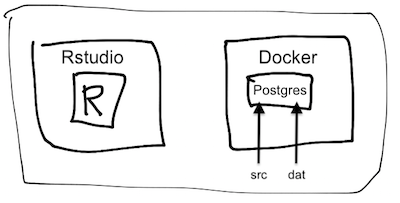
\includegraphics{./screenshots/r-and-docker.png} (This diagram needs to
be updated as our directory structure evolves.)

\hypertarget{who-are-we}{%
\section{Who are we?}\label{who-are-we}}

We have been collaborating on this book since the Summer of 2018, each
of us chipping into the project as time permits:

\begin{itemize}
\tightlist
\item
  Dipti Muni - \href{https://github.com/deemuni}{@deemuni}
\item
  Ian Franz - \href{https://github.com/ianfrantz}{@ianfrantz}
\item
  Jim Tyhurst - \href{https://github.com/jimtyhurst}{@jimtyhurst}
\item
  John David Smith - \href{https://github.com/smithjd}{@smithjd}
\item
  M. Edward (Ed) Borasky - \href{https://github.com/znmeb}{@znmeb}
\item
  Maryann Tygeson \href{https://github.com/maryannet}{@maryannet}
\item
  Scott Came - \href{https://github.com/scottcame}{@scottcame}
\item
  Sophie Yang - \href{https://github.com/SophieMYang}{@SophieMYang}
\end{itemize}

\hypertarget{how-to-use-this-book-01}{%
\chapter{How to use this book (01)}\label{how-to-use-this-book-01}}

This book is full of examples that you can replicate on your computer.

\hypertarget{prerequisites}{%
\section{Prerequisites}\label{prerequisites}}

You will need:

\begin{itemize}
\tightlist
\item
  A computer running Windows, MacOS, or Linux (any Linux distro that
  will run Docker Community Edition, R and RStudio will work)
\item
  \href{https://www.datacamp.com/community/tutorials/installing-R-windows-mac-ubuntu}{R,
  and RStudio}
\item
  Docker
\item
  Our companion package \texttt{sqlpetr} installs with:
  \texttt{devtools::install\_github("smithjd/sqlpetr")}.
\end{itemize}

The database we use is PostgreSQL 10, but you do not need to install
that - it's installed via a Docker image. RStudio 1.2 is highly
recommended but not required.

In addition to the current version of R and RStudio, you will need
current versions of the following packages:

\begin{itemize}
\tightlist
\item
  tidyverse
\item
  DBI
\item
  RPostgres
\item
  glue
\item
  dbplyr
\item
  knitr
\end{itemize}

\hypertarget{installing-docker}{%
\section{Installing Docker}\label{installing-docker}}

Install Docker. Installation depends on your operating system:

\begin{itemize}
\tightlist
\item
  \href{https://docs.docker.com/docker-for-mac/install/}{On a Mac}
\item
  \href{https://docs.docker.com/install/\#supported-platforms}{On UNIX
  flavors}
\item
  For Windows,
  \href{https://smithjd.github.io/sql-pet/docker-hosting-for-windows.html}{consider
  these issues and follow these instructions}.
\end{itemize}

\hypertarget{download-the-repo}{%
\section{Download the repo}\label{download-the-repo}}

The code to generate the book and the exercises it contains can be
downloaded from \href{https://github.com/smithjd/sql-pet}{this repo}.

\hypertarget{read-along-experiment-as-you-go}{%
\section{Read along, experiment as you
go}\label{read-along-experiment-as-you-go}}

We have never been sure whether we're writing an expository book or a
massive tutorial. You may use it either way.

After the introductory chapters and the chapter that creates the
persistent database ("The dvdrental database in Postgres in Docker
(05)), you can jump around and each chapter stands on its own.

\hypertarget{docker-hosting-for-windows-02}{%
\chapter{Docker Hosting for Windows
(02)}\label{docker-hosting-for-windows-02}}

At the end of this chapter, you will be able to

\begin{itemize}
\tightlist
\item
  Setup your environment for Windows.
\item
  Use Git and GitHub effectively on Windows.
\end{itemize}

Skip these instructions if your computer has either OSX or a Unix
variant.

\hypertarget{hardware-requirements}{%
\section{Hardware requirements}\label{hardware-requirements}}

You will need an Intel or AMD processor with 64-bit hardware and the
hardware virtualization feature. Most machines you buy today will have
that, but older ones may not. You will need to go into the BIOS /
firmware and enable the virtualization feature. You will need at least 4
gigabytes of RAM!

\hypertarget{software-requirements}{%
\section{Software requirements}\label{software-requirements}}

You will need Windows 7 64-bit or later. If you can afford it, I highly
recommend upgrading to Windows 10 Pro.

\hypertarget{windows-7-8-8.1-and-windows-10-home-64-bit}{%
\subsection{Windows 7, 8, 8.1 and Windows 10 Home (64
bit)}\label{windows-7-8-8.1-and-windows-10-home-64-bit}}

Install Docker Toolbox. The instructions are here:
\url{https://docs.docker.com/toolbox/toolbox_install_windows/}. Make
sure you try the test cases and they work!

\hypertarget{windows-10-pro}{%
\subsection{Windows 10 Pro}\label{windows-10-pro}}

Install Docker for Windows \emph{stable}. The instructions are here:
\url{https://docs.docker.com/docker-for-windows/install/\#start-docker-for-windows}.
Again, make sure you try the test cases and they work.

\hypertarget{docker-for-windows-settings}{%
\section{Docker for Windows
settings}\label{docker-for-windows-settings}}

\hypertarget{shared-drives}{%
\subsection{Shared drives}\label{shared-drives}}

If you're going to mount host files into container file systems (as we
do in the following chapters), you need to set up shared drives. Open
the Docker settings dialog and select \texttt{Shared\ Drives}. Check the
drives you want to share. In this screenshot, the \texttt{D:} drive is
my 1 terabyte hard drive.

\begin{center}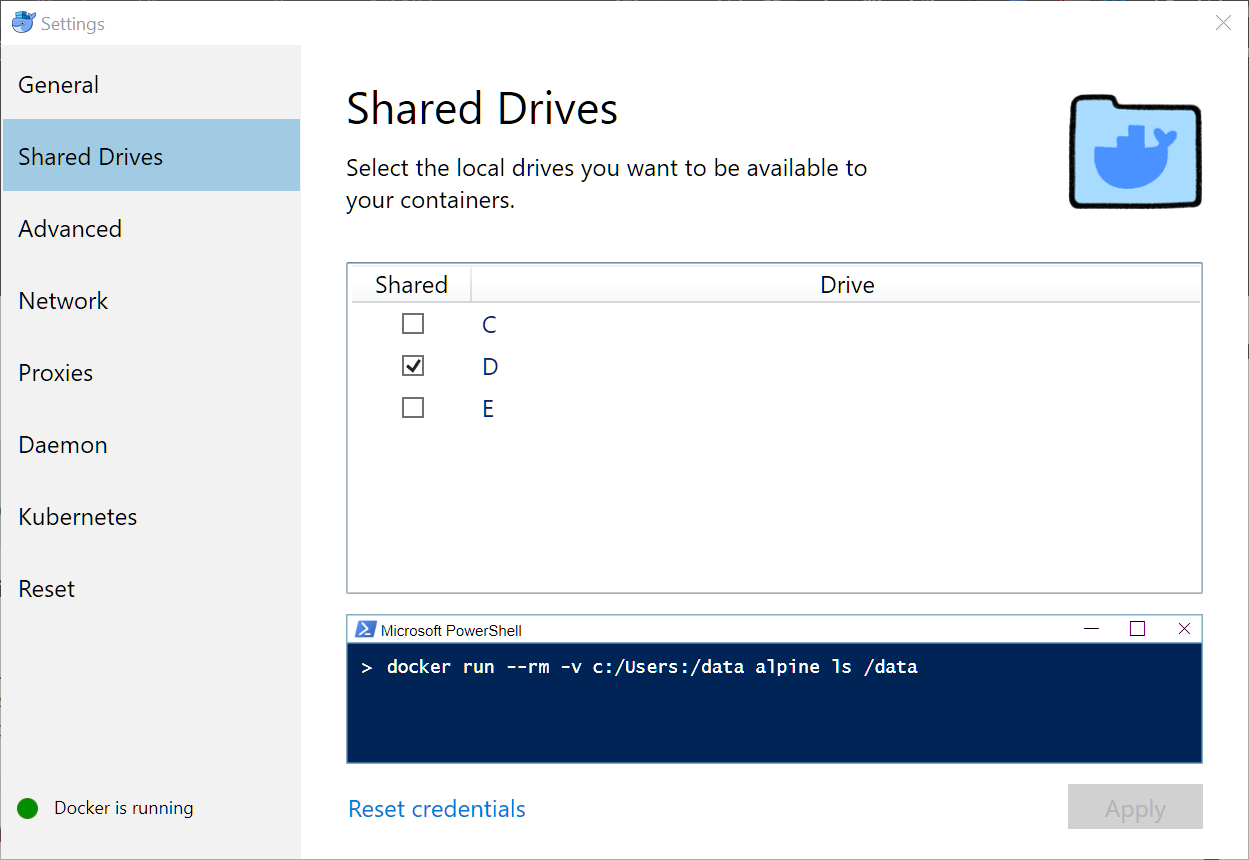
\includegraphics[width=0.9\linewidth]{screenshots/2018-08-26_15_16_51-Shared_Drives} \end{center}

\hypertarget{kubernetes}{%
\subsection{Kubernetes}\label{kubernetes}}

Kubernetes is a container orchestration / cloud management package
that's a major DevOps tool. It's heavily supported by Red Hat and
Google, and as a result is becoming a required skill for DevOps.

However, it's overkill for this project at the moment. So you should
make sure it's not enabled.

Go to the \texttt{Kubernetes} dialog and make sure the
\texttt{Enable\ Kubernetes} checkbox is cleared.

\begin{center}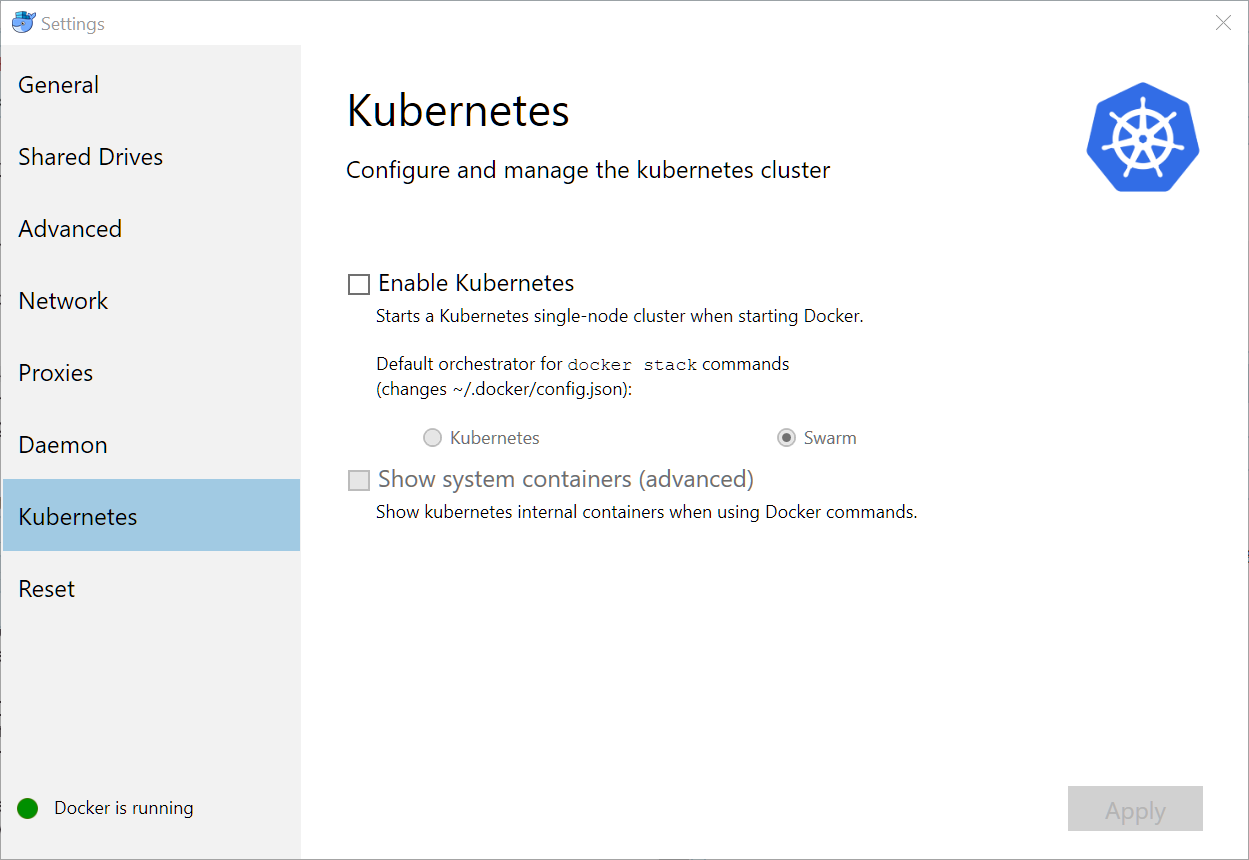
\includegraphics[width=0.9\linewidth]{screenshots/2018-08-26_15_26_22-Kubernetes} \end{center}

\hypertarget{git-github-and-line-endings}{%
\section{Git, GitHub and line
endings}\label{git-github-and-line-endings}}

\href{https://git-scm.com/}{Git} was originally developed for Linux - in
fact, it was created by Linus Torvalds to manage hundreds of different
versions of the Linux kernel on different machines all around the world.
As usage has grown, Git has achieved a huge following and is the version
control system used by most large open source projects, including this
one.

If you're on Windows, there are some things about Git and GitHub you
need to watch. First of all, there are quite a few tools for running Git
on Windows, but the RStudio default and recommended one is Git for
Windows (\url{https://git-scm.com/download/win}).

By default, text files on Linux end with a single linefeed
(\texttt{\textbackslash{}n}) character. But on Windows, text files end
with a carriage return and a line feed
(\texttt{\textbackslash{}r\textbackslash{}n}). See
\url{https://en.wikipedia.org/wiki/Newline} for the gory details.

Git defaults to checking files out in the native mode. So if you're on
Linux, a text file will show up with the Linux convention, and if you're
on Windows, it will show up with the Windows convention.

Most of the time this doesn't cause any problems. But Docker containers
usually run Linux, and if you have files from a repository on Windows
that you've sent to the container, the container may malfunction or give
weird results. \emph{This kind of situation has caused a lot of grief
for contributors to this project, so beware.}

In particular, executable \texttt{sh} or \texttt{bash} scripts will fail
in a Docker container if they have Windows line endings. You may see an
error message with \texttt{\textbackslash{}r} in it, which means the
shell saw the carriage return (\texttt{\textbackslash{}r}) and gave up.
But often you'll see no hint at all what the problem was.

So you need a way to tell Git that some files need to be checked out
with Linux line endings. See
\url{https://help.github.com/articles/dealing-with-line-endings/} for
the details. Summary:

\begin{enumerate}
\def\labelenumi{\arabic{enumi}.}
\tightlist
\item
  You'll need a \texttt{.gitattributes} file in the root of the
  repository.
\item
  In that file, all text files (scripts, program source, data, etc.)
  that are destined for a Docker container will need to have the
  designator \texttt{\textless{}spec\textgreater{}\ text\ eol=lf}, where
  \texttt{\textless{}spec\textgreater{}} is the file name specifier, for
  example, \texttt{*.sh}.
\end{enumerate}

This repo includes a sample:
\href{https://github.com/smithjd/sql-pet/blob/master/.gitattributes}{.gitattributes}

\hypertarget{this-books-learning-goals-and-use-cases-03}{%
\chapter{This Book's Learning Goals and Use Cases
(03)}\label{this-books-learning-goals-and-use-cases-03}}

\hypertarget{learning-goals}{%
\section{Learning Goals}\label{learning-goals}}

After working through this tutorial, you can expect to be able to:

\begin{itemize}
\tightlist
\item
  Set up a PostgreSQL database in a Docker environment.
\item
  Run queries against PostgreSQL in an environment that simulates what
  you will find in a corporate setting.
\item
  Understand techniques and some of the trade-offs between:

  \begin{enumerate}
  \def\labelenumi{\arabic{enumi}.}
  \tightlist
  \item
    queries aimed at exploration or informal investigation using
    \href{https://cran.r-project.org/package=dplyr}{dplyr}; and
  \item
    those where performance is important because of the size of the
    database or the frequency with which a query is run.
  \end{enumerate}
\item
  Understand the equivalence between \texttt{dplyr} and SQL queries and
  how R translates one into the other
\item
  Understand some more advanced SQL techniques.
\item
  Gain familiarity with the standard metadata that an SQL database
  contains to describe its own contents.
\item
  Gain some understanding of techniques for assessing query structure
  and performance.
\item
  Understand enough about Docker to swap databases, e.g.
  \href{http://www.sportsdb.org/sd/samples}{Sports DB} for the
  \href{http://www.postgresqltutorial.com/postgresql-sample-database/}{DVD
  rental database} used in this tutorial. Or swap the database
  management system (DBMS), e.g. \href{https://www.mysql.com/}{MySQL}
  for \href{https://www.postgresql.org/}{PostgreSQL}.
\end{itemize}

\hypertarget{imaging-a-dvd-rental-business}{%
\section{Imaging a DVD rental
business}\label{imaging-a-dvd-rental-business}}

\begin{itemize}
\tightlist
\item
  Years ago people rented videos on DVD disks and video stores were a
  big business.
\item
  Imagine managing a video rental store
  \href{https://en.wikipedia.org/wiki/Movie_Madness_Video}{like Movie
  Madness} in Portland, Oregon.
\end{itemize}

\begin{center}
\includegraphics{screenshots/movie-madness-sample} \end{center}

\begin{itemize}
\tightlist
\item
  What data would be needed and what questions would you have to answer
  about the business?
\end{itemize}

This tutorial uses
\href{http://www.postgresqltutorial.com/postgresql-sample-database/}{the
Postgres version of ``dvd rental'' database} which represents the
transaction database for running a movie (e.g., dvd) rental business.
The database can be
\href{http://www.postgresqltutorial.com/wp-content/uploads/2017/10/dvdrental.zip}{downloaded
here}. Here's a glimpse of it's structure, which will be discussed in
some detail:

\begin{figure}
\centering
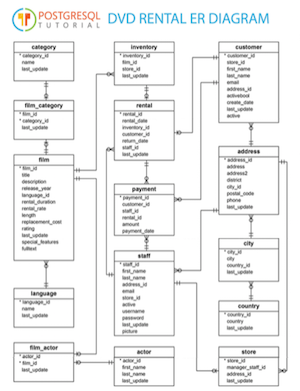
\includegraphics{./screenshots/dvdrental-er-diagram.png}
\caption{Entity Relationship diagram for the dvdrental database}
\end{figure}

A data analyst uses the database abstraction and the practical business
questions to answer business questions.

\hypertarget{use-cases}{%
\section{Use cases}\label{use-cases}}

Imagine that you have one of several roles at our fictional company
\textbf{DVDs R Us} and that you need to:

\begin{itemize}
\tightlist
\item
  As a data scientist, I want to know the distribution of number of
  rentals per month per customer, so that the Marketing department can
  create incentives for customers in 3 segments: Frequent Renters,
  Average Renters, Infrequent Renters.
\item
  As the Director of Sales, I want to see the total number of rentals
  per month for the past 6 months and I want to know how fast our
  customer base is growing/shrinking per month for the past 6 months.
\item
  As the Director of Marketing, I want to know which categories of DVDs
  are the least popular, so that I can create a campaign to draw
  attention to rarely used inventory.
\item
  As a shipping clerk, I want to add rental information when I fulfill a
  shipment order.
\item
  As the Director of Analytics, I want to test as much of the production
  R code in my shop as possible against a new release of the DBMS that
  the IT department is implementing next month.
\item
  etc.
\end{itemize}

\hypertarget{investigating-a-question-using-with-an-organizations-database}{%
\section{Investigating a question using with an organization's
database}\label{investigating-a-question-using-with-an-organizations-database}}

\begin{itemize}
\tightlist
\item
  Need both familiarity with the data and a focus question

  \begin{itemize}
  \tightlist
  \item
    An iterative process where

    \begin{itemize}
    \tightlist
    \item
      the data resource can shape your understanding of the question
    \item
      the question you need to answer will frame how your see the data
      resource
    \end{itemize}
  \item
    You need to go back and forth between the two, asking

    \begin{itemize}
    \tightlist
    \item
      do I understand the question?
    \item
      do I understand the data?
    \end{itemize}
  \end{itemize}
\item
  How well do you understand the data resource (in the DBMS)?

  \begin{itemize}
  \tightlist
  \item
    Use all available documentation and understand its limits
  \item
    Use your own tools and skills to examine the data resource
  \item
    what's \emph{missing} from the database: (columns, records, cells)
  \item
    why is there missing data?
  \end{itemize}
\item
  How well do you understand the question you seek to answer?

  \begin{itemize}
  \tightlist
  \item
    How general or specific is your question?
  \item
    How aligned is it with the purpose for which the database was
    designed and is being operated?
  \item
    How different are your assumptions and concerns from those of the
    people who enter and use the data on a day to day basis?
  \end{itemize}
\end{itemize}

\hypertarget{docker-postgres-and-r-04}{%
\chapter{Docker, Postgres, and R (04)}\label{docker-postgres-and-r-04}}

At the end of this chapter, you will be able to

\begin{itemize}
\tightlist
\item
  Run, clean-up and close Docker containers.
\item
  See how to keep credentials secret in code that's visible to the
  world.
\item
  Interact with Postgres using Rstudio inside Docker container. \# Read
  and write to postgreSQL from R.
\end{itemize}

We always load the tidyverse and some other packages, but don't show it
unless we are using packages other than \texttt{tidyverse},
\texttt{DBI}, \texttt{RPostgres}, and \texttt{glue}.

Devtools install of sqlpetr if not already installed

\hypertarget{verify-that-docker-is-running}{%
\section{Verify that Docker is
running}\label{verify-that-docker-is-running}}

Docker commands can be run from a terminal (e.g., the Rstudio Terminal
pane) or with a \texttt{system()} command. In this tutorial, we use
\texttt{system2()} so that all the output that is created externally is
shown. Note that \texttt{system2} calls are divided into several parts:

\begin{enumerate}
\def\labelenumi{\arabic{enumi}.}
\tightlist
\item
  The program that you are sending a command to.
\item
  The parameters or commands that are being sent.
\item
  \texttt{stdout\ =\ TRUE,\ stderr\ =\ TRUE} are two parameters that are
  standard in this book, so that the command's full output is shown in
  the book.
\end{enumerate}

Check that docker is up and running:

\begin{Shaded}
\begin{Highlighting}[]
\KeywordTok{sp_check_that_docker_is_up}\NormalTok{()}
\end{Highlighting}
\end{Shaded}

\begin{verbatim}
## [1] "Docker is up but running no containers"
\end{verbatim}

\hypertarget{clean-up-if-appropriate}{%
\section{Clean up if appropriate}\label{clean-up-if-appropriate}}

Remove the \texttt{cattle} and \texttt{sql-pet} containers if they
exists (e.g., from a prior experiments).

\begin{Shaded}
\begin{Highlighting}[]
\KeywordTok{sp_docker_remove_container}\NormalTok{(}\StringTok{"cattle"}\NormalTok{)}
\end{Highlighting}
\end{Shaded}

\begin{verbatim}
## Warning in system2("docker", docker_command, stdout = TRUE, stderr = TRUE):
## running command ''docker' rm -f cattle 2>&1' had status 1
\end{verbatim}

\begin{verbatim}
## [1] "Error: No such container: cattle"
## attr(,"status")
## [1] 1
\end{verbatim}

\begin{Shaded}
\begin{Highlighting}[]
\KeywordTok{sp_docker_remove_container}\NormalTok{(}\StringTok{"sql-pet"}\NormalTok{)}
\end{Highlighting}
\end{Shaded}

\begin{verbatim}
## [1] "sql-pet"
\end{verbatim}

The convention we use in this book is to put docker commands in the
\texttt{sqlpetr} package so that you can ignore them if you want.
However, the functions are set up so that you can easily see how to do
things with Docker and modify if you want.

We name containers \texttt{cattle} for ``throw-aways'' and \texttt{pet}
for ones we treasure and keep around. :-)

\begin{Shaded}
\begin{Highlighting}[]
\KeywordTok{sp_make_simple_pg}\NormalTok{(}\StringTok{"cattle"}\NormalTok{)}
\end{Highlighting}
\end{Shaded}

\begin{verbatim}
## [1] 0
\end{verbatim}

Docker returns a long string of numbers. If you are running this command
for the first time, Docker downloads the PostgreSQL image, which takes a
bit of time.

The following command shows that a container named \texttt{cattle} is
running \texttt{postgres:10}. \texttt{postgres} is waiting for a
connection:

\begin{Shaded}
\begin{Highlighting}[]
\KeywordTok{sp_check_that_docker_is_up}\NormalTok{()}
\end{Highlighting}
\end{Shaded}

\begin{verbatim}
## [1] "Docker is up, running these containers:"                                                                                                       
## [2] "CONTAINER ID        IMAGE               COMMAND                  CREATED             STATUS                  PORTS                    NAMES"   
## [3] "c9033dd56c41        postgres:10         \"docker-entrypoint.s…\"   1 second ago        Up Less than a second   0.0.0.0:5432->5432/tcp   cattle"
\end{verbatim}

\hypertarget{connect-read-and-write-to-postgres-from-r}{%
\section{Connect, read and write to Postgres from
R}\label{connect-read-and-write-to-postgres-from-r}}

\hypertarget{pause-for-some-security-considerations}{%
\subsection{Pause for some security
considerations}\label{pause-for-some-security-considerations}}

We use the following \texttt{sp\_get\_postgres\_connection} function,
which will repeatedly try to connect to PostgreSQL. PostgreSQL can take
different amounts of time to come up and be ready to accept connections
from R, depending on various factors that will be discussed later on.

This is how the \texttt{sp\_get\_postgres\_connection} function is used:

\begin{Shaded}
\begin{Highlighting}[]
\NormalTok{con <-}\StringTok{ }\KeywordTok{sp_get_postgres_connection}\NormalTok{(}\DataTypeTok{user =} \KeywordTok{Sys.getenv}\NormalTok{(}\StringTok{"DEFAULT_POSTGRES_USER_NAME"}\NormalTok{),}
                         \DataTypeTok{password =} \KeywordTok{Sys.getenv}\NormalTok{(}\StringTok{"DEFAULT_POSTGRES_PASSWORD"}\NormalTok{),}
                         \DataTypeTok{dbname =} \StringTok{"postgres"}\NormalTok{,}
                         \DataTypeTok{seconds_to_test =} \DecValTok{10}\NormalTok{)}
\end{Highlighting}
\end{Shaded}

If you don't have an \texttt{.Rprofile} file that defines those
passwords, you can just insert a string for the parameter, like:

\texttt{password\ =\ \textquotesingle{}whatever\textquotesingle{},}

Make sure that you can connect to the PostgreSQL database that you
started earlier. If you have been executing the code from this tutorial,
the database will not contain any tables yet:

\begin{Shaded}
\begin{Highlighting}[]
\KeywordTok{dbListTables}\NormalTok{(con)}
\end{Highlighting}
\end{Shaded}

\begin{verbatim}
## character(0)
\end{verbatim}

\hypertarget{alternative-put-the-database-password-in-an-environment-file}{%
\subsection{Alternative: put the database password in an environment
file}\label{alternative-put-the-database-password-in-an-environment-file}}

The goal is to put the password in an untracked file that will
\textbf{not} be committed in your source code repository. Your code can
reference the name of the variable, but the value of that variable will
not appear in open text in your source code.

We have chosen to call the file \texttt{dev\_environment.csv} in the
current working directory where you are executing this script. That file
name appears in the \texttt{.gitignore} file, so that you will not
accidentally commit it. We are going to create that file now.

You will be prompted for the database password. By default, a PostgreSQL
database defines a database user named \texttt{postgres}, whose password
is \texttt{postgres}. If you have changed the password or created a new
user with a different password, then enter those new values when
prompted. Otherwise, enter \texttt{postgres} and \texttt{postgres} at
the two prompts.

In an interactive environment, you could execute a snippet of code that
prompts the user for their username and password with the following
snippet (which isn't run in the book):

Your password is still in plain text in the file,
\texttt{dev\_environment.csv}, so you should protect that file from
exposure. However, you do not need to worry about committing that file
accidentally to your git repository, because the name of the file
appears in the \texttt{.gitignore} file.

For security, we use values from the \texttt{environment\_variables}
data.frame, rather than keeping the \texttt{username} and
\texttt{password} in plain text in a source file.

\hypertarget{interact-with-postgres}{%
\subsection{Interact with Postgres}\label{interact-with-postgres}}

Write \texttt{mtcars} to PostgreSQL

\begin{Shaded}
\begin{Highlighting}[]
\KeywordTok{dbWriteTable}\NormalTok{(con, }\StringTok{"mtcars"}\NormalTok{, mtcars, }\DataTypeTok{overwrite =} \OtherTok{TRUE}\NormalTok{)}
\end{Highlighting}
\end{Shaded}

List the tables in the PostgreSQL database to show that \texttt{mtcars}
is now there:

\begin{Shaded}
\begin{Highlighting}[]
\KeywordTok{dbListTables}\NormalTok{(con)}
\end{Highlighting}
\end{Shaded}

\begin{verbatim}
## [1] "mtcars"
\end{verbatim}

\begin{Shaded}
\begin{Highlighting}[]
\CommentTok{# list the fields in mtcars:}
\KeywordTok{dbListFields}\NormalTok{(con, }\StringTok{"mtcars"}\NormalTok{)}
\end{Highlighting}
\end{Shaded}

\begin{verbatim}
##  [1] "mpg"  "cyl"  "disp" "hp"   "drat" "wt"   "qsec" "vs"   "am"   "gear"
## [11] "carb"
\end{verbatim}

Download the table from the DBMS to a local data frame:

\begin{Shaded}
\begin{Highlighting}[]
\NormalTok{mtcars_df <-}\StringTok{ }\KeywordTok{tbl}\NormalTok{(con, }\StringTok{"mtcars"}\NormalTok{)}

\CommentTok{# Show a few rows:}
\NormalTok{knitr}\OperatorTok{::}\KeywordTok{kable}\NormalTok{(}\KeywordTok{head}\NormalTok{(mtcars_df))}
\end{Highlighting}
\end{Shaded}

\begin{tabular}{r|r|r|r|r|r|r|r|r|r|r}
\hline
mpg & cyl & disp & hp & drat & wt & qsec & vs & am & gear & carb\\
\hline
21.0 & 6 & 160 & 110 & 3.90 & 2.620 & 16.46 & 0 & 1 & 4 & 4\\
\hline
21.0 & 6 & 160 & 110 & 3.90 & 2.875 & 17.02 & 0 & 1 & 4 & 4\\
\hline
22.8 & 4 & 108 & 93 & 3.85 & 2.320 & 18.61 & 1 & 1 & 4 & 1\\
\hline
21.4 & 6 & 258 & 110 & 3.08 & 3.215 & 19.44 & 1 & 0 & 3 & 1\\
\hline
18.7 & 8 & 360 & 175 & 3.15 & 3.440 & 17.02 & 0 & 0 & 3 & 2\\
\hline
18.1 & 6 & 225 & 105 & 2.76 & 3.460 & 20.22 & 1 & 0 & 3 & 1\\
\hline
\end{tabular}

\hypertarget{clean-up}{%
\section{Clean up}\label{clean-up}}

Afterwards, always disconnect from the DBMS, stop the docker container
and (optionally) remove it.

\begin{Shaded}
\begin{Highlighting}[]
\KeywordTok{dbDisconnect}\NormalTok{(con)}

\CommentTok{# tell Docker to stop the container:}
\KeywordTok{sp_docker_stop}\NormalTok{(}\StringTok{"cattle"}\NormalTok{)}
\end{Highlighting}
\end{Shaded}

\begin{verbatim}
## [1] "cattle"
\end{verbatim}

\begin{Shaded}
\begin{Highlighting}[]
\CommentTok{# Tell Docker to remove the container from it's library of active containers:}
\KeywordTok{sp_docker_remove_container}\NormalTok{(}\StringTok{"cattle"}\NormalTok{)}
\end{Highlighting}
\end{Shaded}

\begin{verbatim}
## [1] "cattle"
\end{verbatim}

If we \texttt{stop} the docker container but don't remove it (with the
\texttt{rm\ cattle} command), the container will persist and we can
start it up again later with \texttt{start\ cattle}. In that case,
\texttt{mtcars} would still be there and we could retrieve it from R
again. Since we have now removed the \texttt{cattle} container, the
whole database has been deleted. (There are enough copies of
\texttt{mtcars} in the world, so no great loss.)

\hypertarget{a-persistent-database-in-postgres-in-docker---all-at-once-05}{%
\chapter{A persistent database in Postgres in Docker - all at once
(05)}\label{a-persistent-database-in-postgres-in-docker---all-at-once-05}}

At the end of this chapter, you will be able to

\begin{itemize}
\tightlist
\item
  Setup a database with ``all in one'' approach.
\item
  Stop and start Docker image to demonstrate persistence
\item
  Disconnect R from database and stop container to close up even though
  it still exists.
\end{itemize}

\hypertarget{overview}{%
\section{Overview}\label{overview}}

You've already connected to PostgreSQL with R, now you need a
``realistic'' (\texttt{dvdrental}) database. We're going to demonstrate
how to set one up, with two different approaches. This chapter and the
next do the same job, illustrating the different approaches that you can
take and helping you see the different points where you could swap
what's provided here with a different DBMS or a different backup file or
something else.

The code in this first version is recommended because it is an ``all in
one'' approach. Details about how it works and how you might modify it
are included below. There is another version in the the next chapter
that you can use to investigate Docker commands and components.

Note that \texttt{tidyverse}, \texttt{DBI}, \texttt{RPostgres}, and
\texttt{glue} are loaded.

\hypertarget{verify-that-docker-is-up-and-running}{%
\section{Verify that Docker is up and
running}\label{verify-that-docker-is-up-and-running}}

\begin{Shaded}
\begin{Highlighting}[]
\KeywordTok{sp_check_that_docker_is_up}\NormalTok{()}
\end{Highlighting}
\end{Shaded}

\begin{verbatim}
## [1] "Docker is up but running no containers"
\end{verbatim}

\hypertarget{clean-up-if-appropriate-1}{%
\section{Clean up if appropriate}\label{clean-up-if-appropriate-1}}

Remove the \texttt{sql-pet} container if it exists (e.g., from a prior
run)

\begin{Shaded}
\begin{Highlighting}[]
\KeywordTok{sp_docker_remove_container}\NormalTok{(}\StringTok{"sql-pet"}\NormalTok{)}
\end{Highlighting}
\end{Shaded}

\begin{verbatim}
## Warning in system2("docker", docker_command, stdout = TRUE, stderr = TRUE):
## running command ''docker' rm -f sql-pet 2>&1' had status 1
\end{verbatim}

\begin{verbatim}
## [1] "Error: No such container: sql-pet"
## attr(,"status")
## [1] 1
\end{verbatim}

\hypertarget{build-the-docker-image}{%
\section{Build the Docker Image}\label{build-the-docker-image}}

Build an image that derives from postgres:10, defined in
\texttt{dvdrental.Dockerfile}, that is set up to restore and load the
dvdrental db on startup. The
\href{./dvdrental.Dockerfile}{dvdrental.Dockerfile} is discussed below.

\begin{Shaded}
\begin{Highlighting}[]
\KeywordTok{system2}\NormalTok{(}\StringTok{"docker"}\NormalTok{, }
        \KeywordTok{glue}\NormalTok{(}\StringTok{"build "}\NormalTok{, }\CommentTok{# tells Docker to build an image that can be loaded as a container}
          \StringTok{"--tag postgres-dvdrental "}\NormalTok{, }\CommentTok{# (or -t) tells Docker to name the image}
          \StringTok{"--file dvdrental.Dockerfile "}\NormalTok{, }\CommentTok{#(or -f) tells Docker to read `build` instructions from the dvdrental.Dockerfile}
          \StringTok{" . "}\NormalTok{),  }\CommentTok{# tells Docker to look for dvdrental.Dockerfile in the current directory}
          \DataTypeTok{stdout =} \OtherTok{TRUE}\NormalTok{, }\DataTypeTok{stderr =} \OtherTok{TRUE}\NormalTok{)}
\end{Highlighting}
\end{Shaded}

\begin{verbatim}
##  [1] "Sending build context to Docker daemon  32.44MB\r\r"                                                                                                                                                                                                                                                                                                                                           
##  [2] "Step 1/4 : FROM postgres:10"                                                                                                                                                                                                                                                                                                                                                                   
##  [3] " ---> ac25c2bac3c4"                                                                                                                                                                                                                                                                                                                                                                            
##  [4] "Step 2/4 : WORKDIR /tmp"                                                                                                                                                                                                                                                                                                                                                                       
##  [5] " ---> Using cache"                                                                                                                                                                                                                                                                                                                                                                             
##  [6] " ---> 3f00a18e0bdf"                                                                                                                                                                                                                                                                                                                                                                            
##  [7] "Step 3/4 : COPY init-dvdrental.sh /docker-entrypoint-initdb.d/"                                                                                                                                                                                                                                                                                                                                
##  [8] " ---> Using cache"                                                                                                                                                                                                                                                                                                                                                                             
##  [9] " ---> 3453d61d8e3e"                                                                                                                                                                                                                                                                                                                                                                            
## [10] "Step 4/4 : RUN apt-get -qq update &&   apt-get install -y -qq curl zip  > /dev/null 2>&1 &&   curl -Os http://www.postgresqltutorial.com/wp-content/uploads/2017/10/dvdrental.zip &&   unzip dvdrental.zip &&   rm dvdrental.zip &&   chmod ugo+w dvdrental.tar &&   chown postgres dvdrental.tar &&   chmod u+x /docker-entrypoint-initdb.d/init-dvdrental.sh &&   apt-get remove -y curl zip"
## [11] " ---> Using cache"                                                                                                                                                                                                                                                                                                                                                                             
## [12] " ---> f5e93aa64875"                                                                                                                                                                                                                                                                                                                                                                            
## [13] "Successfully built f5e93aa64875"                                                                                                                                                                                                                                                                                                                                                               
## [14] "Successfully tagged postgres-dvdrental:latest"
\end{verbatim}

\hypertarget{run-the-docker-image}{%
\section{Run the Docker Image}\label{run-the-docker-image}}

Run docker to bring up postgres. The first time it runs it will take a
minute to create the PostgreSQL environment. There are two important
parts to this that may not be obvious:

\begin{itemize}
\tightlist
\item
  The \texttt{source=} parameter points to
  \href{./dvdrental.Dockerfile}{dvdrental.Dockerfile}, which does most
  of the heavy lifting. It has detailed, line-by-line comments to
  explain what it is doing.\\
\item
  \emph{Inside} \href{./dvdrental.Dockerfile}{dvdrental.Dockerfile} the
  command \texttt{COPY\ init-dvdrental.sh\ /docker-entrypoint-initdb.d/}
  copies \url{init-dvdrental.sh} from the local file system into the
  specified location in the Docker container. When the PostgreSQL Docker
  container initializes, it looks for that file and executes it.
\end{itemize}

Doing all of that work behind the scenes involves two layers of
complexity. Depending on how you look at it, that may be more or less
difficult to understand than the method shown in the next Chapter.

\begin{Shaded}
\begin{Highlighting}[]
\NormalTok{wd <-}\StringTok{ }\KeywordTok{getwd}\NormalTok{()}

\NormalTok{docker_cmd <-}\StringTok{ }\KeywordTok{glue}\NormalTok{(}
  \StringTok{"run "}\NormalTok{,      }\CommentTok{# Run is the Docker command.  Everything that follows are `run` parameters.}
  \StringTok{"--detach "}\NormalTok{, }\CommentTok{# (or `-d`) tells Docker to disconnect from the terminal / program issuing the command}
  \StringTok{" --name sql-pet "}\NormalTok{,     }\CommentTok{# tells Docker to give the container a name: `sql-pet`}
  \StringTok{"--publish 5432:5432 "}\NormalTok{, }\CommentTok{# tells Docker to expose the Postgres port 5432 to the local network with 5432}
  \StringTok{"--mount "}\NormalTok{, }\CommentTok{# tells Docker to mount a volume -- mapping Docker's internal file structure to the host file structure}
  \StringTok{"type=bind,"}\NormalTok{, }\CommentTok{# tells Docker that the mount command points to an actual file on the host system}
  \StringTok{'source="'}\NormalTok{, }\CommentTok{# tells Docker where the local file will be found}
\NormalTok{  wd, }\StringTok{'/",'}\NormalTok{, }\CommentTok{# the current working directory, as retrieved above}
  \StringTok{"target=/petdir"}\NormalTok{, }\CommentTok{# tells Docker to refer to the current directory as "/petdir" in its file system}
  \StringTok{" postgres-dvdrental"} \CommentTok{# tells Docker to run the image was built in the previous step}
\NormalTok{)}

\CommentTok{# if you are curious you can paste this string into a terminal window after the command 'docker':}
\NormalTok{docker_cmd}
\end{Highlighting}
\end{Shaded}

\begin{verbatim}
## run --detach  --name sql-pet --publish 5432:5432 --mount type=bind,source="/Users/jds/Documents/Library/R/r-system/sql-pet/",target=/petdir postgres-dvdrental
\end{verbatim}

\begin{Shaded}
\begin{Highlighting}[]
\KeywordTok{system2}\NormalTok{(}\StringTok{"docker"}\NormalTok{, docker_cmd, }\DataTypeTok{stdout =} \OtherTok{TRUE}\NormalTok{, }\DataTypeTok{stderr =} \OtherTok{TRUE}\NormalTok{)}
\end{Highlighting}
\end{Shaded}

\begin{verbatim}
## [1] "55ba7582259addf380fee1980edfc9b4d1e0bf80f8a99f4cb599eeb754c56aa0"
\end{verbatim}

\hypertarget{connect-to-postgres-with-r}{%
\section{Connect to Postgres with R}\label{connect-to-postgres-with-r}}

Use the DBI package to connect to PostgreSQL. But first, wait for Docker
\& PostgreSQL to come up before connecting.

We have loaded the \texttt{wait\_for\_postgres} function behind the
scenes.

\begin{Shaded}
\begin{Highlighting}[]
\NormalTok{con <-}\StringTok{ }\KeywordTok{sp_get_postgres_connection}\NormalTok{(}\DataTypeTok{user =} \KeywordTok{Sys.getenv}\NormalTok{(}\StringTok{"DEFAULT_POSTGRES_USER_NAME"}\NormalTok{),}
                         \DataTypeTok{password =} \KeywordTok{Sys.getenv}\NormalTok{(}\StringTok{"DEFAULT_POSTGRES_PASSWORD"}\NormalTok{),}
                         \DataTypeTok{dbname =} \StringTok{"dvdrental"}\NormalTok{,}
                         \DataTypeTok{seconds_to_test =} \DecValTok{10}\NormalTok{)}

\KeywordTok{dbListTables}\NormalTok{(con)}
\end{Highlighting}
\end{Shaded}

\begin{verbatim}
##  [1] "actor_info"                 "customer_list"             
##  [3] "film_list"                  "nicer_but_slower_film_list"
##  [5] "sales_by_film_category"     "staff"                     
##  [7] "sales_by_store"             "staff_list"                
##  [9] "category"                   "film_category"             
## [11] "country"                    "actor"                     
## [13] "language"                   "inventory"                 
## [15] "payment"                    "rental"                    
## [17] "city"                       "store"                     
## [19] "film"                       "address"                   
## [21] "film_actor"                 "customer"
\end{verbatim}

\begin{Shaded}
\begin{Highlighting}[]
\KeywordTok{dbListFields}\NormalTok{(con, }\StringTok{"rental"}\NormalTok{)}
\end{Highlighting}
\end{Shaded}

\begin{verbatim}
## [1] "rental_id"    "rental_date"  "inventory_id" "customer_id" 
## [5] "return_date"  "staff_id"     "last_update"
\end{verbatim}

\begin{Shaded}
\begin{Highlighting}[]
\KeywordTok{dbDisconnect}\NormalTok{(con)}
\end{Highlighting}
\end{Shaded}

\hypertarget{stop-and-start-to-demonstrate-persistence}{%
\section{Stop and start to demonstrate
persistence}\label{stop-and-start-to-demonstrate-persistence}}

Stop the container

\begin{Shaded}
\begin{Highlighting}[]
\KeywordTok{sp_docker_stop}\NormalTok{(}\StringTok{"sql-pet"}\NormalTok{)}
\end{Highlighting}
\end{Shaded}

\begin{verbatim}
## [1] "sql-pet"
\end{verbatim}

Restart the container and verify that the dvdrental tables are still
there

\begin{Shaded}
\begin{Highlighting}[]
\KeywordTok{sp_docker_start}\NormalTok{(}\StringTok{"sql-pet"}\NormalTok{)}

\NormalTok{con <-}\StringTok{ }\KeywordTok{sp_get_postgres_connection}\NormalTok{(}\DataTypeTok{user =} \KeywordTok{Sys.getenv}\NormalTok{(}\StringTok{"DEFAULT_POSTGRES_USER_NAME"}\NormalTok{),}
                         \DataTypeTok{password =} \KeywordTok{Sys.getenv}\NormalTok{(}\StringTok{"DEFAULT_POSTGRES_PASSWORD"}\NormalTok{),}
                         \DataTypeTok{dbname =} \StringTok{"dvdrental"}\NormalTok{,}
                         \DataTypeTok{seconds_to_test =} \DecValTok{10}\NormalTok{)}

\KeywordTok{glimpse}\NormalTok{(}\KeywordTok{dbReadTable}\NormalTok{(con, }\StringTok{"film"}\NormalTok{))}
\end{Highlighting}
\end{Shaded}

\begin{verbatim}
## Observations: 1,000
## Variables: 13
## $ film_id          <int> 133, 384, 8, 98, 1, 2, 3, 4, 5, 6, 7, 9, 10, ...
## $ title            <chr> "Chamber Italian", "Grosse Wonderful", "Airpo...
## $ description      <chr> "A Fateful Reflection of a Moose And a Husban...
## $ release_year     <int> 2006, 2006, 2006, 2006, 2006, 2006, 2006, 200...
## $ language_id      <int> 1, 1, 1, 1, 1, 1, 1, 1, 1, 1, 1, 1, 1, 1, 1, ...
## $ rental_duration  <int> 7, 5, 6, 4, 6, 3, 7, 5, 6, 3, 6, 3, 6, 6, 6, ...
## $ rental_rate      <dbl> 4.99, 4.99, 4.99, 4.99, 0.99, 4.99, 2.99, 2.9...
## $ length           <int> 117, 49, 54, 73, 86, 48, 50, 117, 130, 169, 6...
## $ replacement_cost <dbl> 14.99, 19.99, 15.99, 12.99, 20.99, 12.99, 18....
## $ rating           <chr> "NC-17", "R", "R", "PG-13", "PG", "G", "NC-17...
## $ last_update      <dttm> 2013-05-26 14:50:58, 2013-05-26 14:50:58, 20...
## $ special_features <chr> "{Trailers}", "{\"Behind the Scenes\"}", "{Tr...
## $ fulltext         <chr> "'chamber':1 'fate':4 'husband':11 'italian':...
\end{verbatim}

\hypertarget{cleaning-up}{%
\section{Cleaning up}\label{cleaning-up}}

It's always good to have R disconnect from the database

\begin{Shaded}
\begin{Highlighting}[]
\KeywordTok{dbDisconnect}\NormalTok{(con)}
\end{Highlighting}
\end{Shaded}

Stop the container and show that the container is still there, so can be
started again.

\begin{Shaded}
\begin{Highlighting}[]
\KeywordTok{sp_docker_stop}\NormalTok{(}\StringTok{"sql-pet"}\NormalTok{)}
\end{Highlighting}
\end{Shaded}

\begin{verbatim}
## [1] "sql-pet"
\end{verbatim}

\begin{Shaded}
\begin{Highlighting}[]
\CommentTok{# show that the container still exists even though it's not running}
\KeywordTok{sp_show_all_docker_containers}\NormalTok{()}
\end{Highlighting}
\end{Shaded}

\begin{verbatim}
## [1] "CONTAINER ID        IMAGE                COMMAND                  CREATED             STATUS                              PORTS               NAMES"    
## [2] "55ba7582259a        postgres-dvdrental   \"docker-entrypoint.s…\"   7 seconds ago       Exited (0) Less than a second ago                       sql-pet"
\end{verbatim}

Next time, you can just use this command to start the container:

\texttt{sp\_docker\_start("sql-pet")}

And once stopped, the container can be removed with:

\texttt{sp\_check\_that\_docker\_is\_up("sql-pet)}

\hypertarget{using-the-sql-pet-container-in-the-rest-of-the-book}{%
\section{\texorpdfstring{Using the \texttt{sql-pet} container in the
rest of the
book}{Using the sql-pet container in the rest of the book}}\label{using-the-sql-pet-container-in-the-rest-of-the-book}}

After this point in the book, we assume that Docker is up and that we
can always start up our \emph{sql-pet database} with:

\texttt{sp\_docker\_stop("sql-pet")}

\hypertarget{mapping-your-local-environment-10}{%
\chapter{Mapping your local environment
(10)}\label{mapping-your-local-environment-10}}

\hypertarget{basics}{%
\section{Basics}\label{basics}}

\begin{itemize}
\tightlist
\item
  Keeping passwords secure.
\item
  Coverage in this book. There are many SQL tutorials that are
  available. For example, we are drawing some materials from
  \href{http://www.postgresqltutorial.com/postgresql-sample-database/}{a
  tutorial we recommend}. In particular, we will not replicate the
  lessons there, which you might want to complete. Instead, we are
  showing strategies that are recommended for R users. That will include
  some translations of queries that are discussed there.
\end{itemize}

\hypertarget{ask-yourself-what-are-you-aiming-for}{%
\section{Ask yourself, what are you aiming
for?}\label{ask-yourself-what-are-you-aiming-for}}

\begin{itemize}
\tightlist
\item
  Differences between production and data warehouse environments.
\item
  Learning to keep your DBAs happy:

  \begin{itemize}
  \tightlist
  \item
    You are your own DBA in this simulation, so you can wreak havoc and
    learn from it, but you can learn to be DBA-friendly here.
  \item
    In the end it's the subject-matter experts that understand your
    data, but you have to work with your DBAs first.
  \end{itemize}
\end{itemize}

\hypertarget{get-some-basic-information-about-your-database}{%
\section{Get some basic information about your
database}\label{get-some-basic-information-about-your-database}}

Assume that the Docker container with PostgreSQL and the dvdrental
database are ready to go. Start up the \texttt{docker-pet} container

\begin{Shaded}
\begin{Highlighting}[]
\KeywordTok{sp_docker_start}\NormalTok{(}\StringTok{"sql-pet"}\NormalTok{)}
\end{Highlighting}
\end{Shaded}

Now connect to the \texttt{dvdrental} database with R

\begin{Shaded}
\begin{Highlighting}[]
\NormalTok{con <-}\StringTok{ }\KeywordTok{sp_get_postgres_connection}\NormalTok{(}
  \DataTypeTok{user =} \KeywordTok{Sys.getenv}\NormalTok{(}\StringTok{"DEFAULT_POSTGRES_USER_NAME"}\NormalTok{),}
  \DataTypeTok{password =}  \KeywordTok{Sys.getenv}\NormalTok{(}\StringTok{"DEFAULT_POSTGRES_PASSWORD"}\NormalTok{),}
  \DataTypeTok{dbname =} \StringTok{"dvdrental"}\NormalTok{,}
  \DataTypeTok{seconds_to_test =} \DecValTok{10}\NormalTok{)}
\NormalTok{con}
\end{Highlighting}
\end{Shaded}

\begin{verbatim}
## <PqConnection> dvdrental@localhost:5432
\end{verbatim}

The following code block confirms that one can connect to the Postgres
database. The connection is needed for some of the examples/exercises
used in this section. If the connection is successful, the output is
\texttt{\textless{}PostgreSQLConnection\textgreater{}}.

\hypertarget{tutorial-environment}{%
\section{Tutorial Environment}\label{tutorial-environment}}

Below is a high level diagram of our tutorial environment. The single
black or blue boxed items are the apps running on your PC, (Linux, Mac,
Windows), RStudio, R, Docker, and CLI, a command line interface. The red
boxed items are the versions of the applications shown. The labels are
to the right of the line.

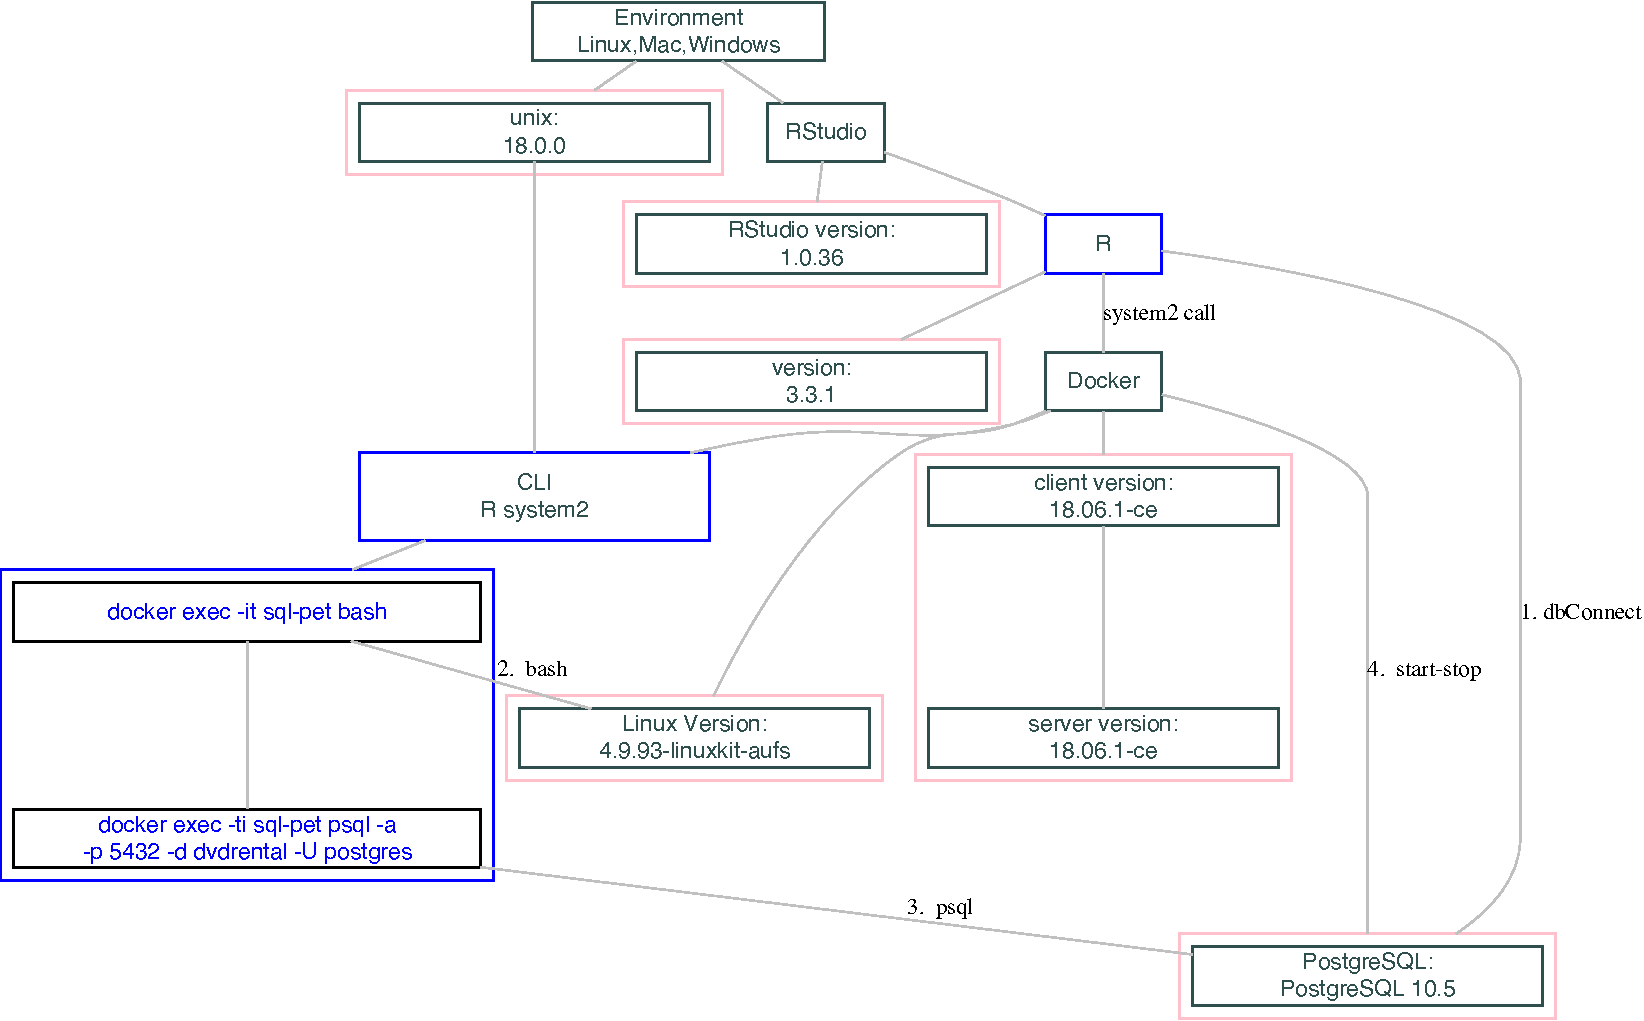
\includegraphics{10-environment_diagram_files/figure-latex/Environment Graph-1.pdf}

\hypertarget{communicating-with-docker-applications}{%
\section{Communicating with Docker
Applications}\label{communicating-with-docker-applications}}

One assumption we made is that most users use \texttt{RStudio} to
interface with \texttt{R}. The four take aways from the diagram above
are labeled:

\begin{enumerate}
\def\labelenumi{\arabic{enumi}.}
\tightlist
\item
  dbConnect
\end{enumerate}

R-SQL processing, the purpose of this tutorial, is performed via a
database connection. This should be a simple task, but often turns out
to take a lot of time to actually get it to work. We assume that your
final write ups are done in some flavor of an Rmd document and others
will have access to the database to confirm or further your analysis.

For this tutorial, the following are the hardcoded values used to make
the Postgres database connection.

\begin{verbatim}
    con <- sp_get_postgres_connection(
      user = Sys.getenv("DEFAULT_POSTGRES_USER_NAME"),
      password =  Sys.getenv("DEFAULT_POSTGRES_PASSWORD"),
      dbname = "dvdrental",
      seconds_to_test = 10)
\end{verbatim}

The main focus of the entire tutorial is SQL processing through a
dbConnection. The remainder of this section focuses on some specific
Docker commands.

\begin{enumerate}
\def\labelenumi{\arabic{enumi}.}
\setcounter{enumi}{1}
\tightlist
\item
  bash
\end{enumerate}

The Docker container runs on top of a small Linux kernel foot print.
Since Mac and Linux users run a version of Linux already, they may want
to poke around the Docker environment. Below is the CLI command to start
up a bash session, execute a version of hello world, and exit the
\texttt{bash} session.

\begin{verbatim}
c:\Git\sql-pet>docker exec -ti sql-pet bash
root@7e43294b72cf:/# echo "'hello world'" talking to you live from a bash shell session within Docker!
'hello world' talking to you live from a bash shell session within Docker!
root@7e43294b72cf:/# exit
exit
\end{verbatim}

Note that the user in the example is root. Root has all priviledges and
can destroy the Docker environment.

\begin{enumerate}
\def\labelenumi{\arabic{enumi}.}
\setcounter{enumi}{2}
\tightlist
\item
  psql
\end{enumerate}

For users comfortable executing SQL from a command line directly against
the database, one can run the \texttt{psql} application directly. Below
is the CLI command to start up \texttt{psql} session, execute a version
of hello world, and quitting the \texttt{psql} version.

\begin{verbatim}
c:\Git\sql-pet>docker exec -ti sql-pet psql -a -p 5432 -d dvdrental -U postgres
psql (10.5 (Debian 10.5-1.pgdg90+1))
Type "help" for help.

dvdrental=# select '"hello world" talking to you live from postgres session within Docker!' hello;
                                hello
------------------------------------------------------------------------
 "hello world" talking to you live from postgres session within Docker!
(1 row)

dvdrental=# \q
\end{verbatim}

All SQL commands need to end with a semi-colon. To exit \texttt{psql},
use a `\q' at the command prompt.

The docker bash and psql command options are optional for this tutorial,
but open up a gateway to some very powerful programming techniques for
future exploration.

\begin{enumerate}
\def\labelenumi{\arabic{enumi}.}
\setcounter{enumi}{3}
\tightlist
\item
  start-stop
\end{enumerate}

Docker has about 44 commands. We are interested in only those related to
Postgres status, started, stopped, and available. In this tutorial,
complete docker commands are printed out before being executed via a
\texttt{system2} call. In the event that a code block fails, one can
copy and paste the docker command into your local CLI and see if Docker
is returning additional information.

\hypertarget{exercises}{%
\section{Exercises}\label{exercises}}

Docker containers have a small foot print. In our container, we are
running a limited Linux kernel and a Postgres database. To show how tiny
the docker environment is, we will look at all the processes running
inside Docker and the top level file structure.

\hypertarget{docker-help}{%
\subsection{Docker Help}\label{docker-help}}

Typing \texttt{docker} at the command line will print up a summary of
all available \texttt{docker} commands. Below are the docker commands
used in the exercises.

\begin{verbatim}
Commands:
  ps          List containers
  start       Start one or more stopped containers
  stop        Stop one or more running containers
\end{verbatim}

The general format for a Docker command is

\begin{verbatim}
docker [OPTIONS] COMMAND ARGUMENTS
\end{verbatim}

Below is the output for the Docker exec help command which was used in
the \texttt{bash} and \texttt{psql} command examples above and for an
exercise below.

\begin{verbatim}
C:\Users\SMY>docker help exec

Usage:  docker exec [OPTIONS] CONTAINER COMMAND [ARG...]

Run a command in a running container

Options:
  -d, --detach               Detached mode: run command in the background
      --detach-keys string   Override the key sequence for detaching a
                             container
  -e, --env list             Set environment variables
  -i, --interactive          Keep STDIN open even if not attached
      --privileged           Give extended privileges to the command
  -t, --tty                  Allocate a pseudo-TTY
  -u, --user string          Username or UID (format:
                             <name|uid>[:<group|gid>])
  -w, --workdir string       Working directory inside the container
\end{verbatim}

In these exercies, the \texttt{-i} option and the CONTAINER =
\texttt{sql-pet} are used in two of the exercises.

Start up R/RStudio and convert the CLI command to an R/RStudio command

\begin{longtable}[]{@{}lllll@{}}
\toprule
\begin{minipage}[b]{0.02\columnwidth}\raggedright
\#\strut
\end{minipage} & \begin{minipage}[b]{0.19\columnwidth}\raggedright
Question\strut
\end{minipage} & \begin{minipage}[b]{0.29\columnwidth}\raggedright
Docker CLI Command\strut
\end{minipage} & \begin{minipage}[b]{0.20\columnwidth}\raggedright
R RStudio command\strut
\end{minipage} & \begin{minipage}[b]{0.16\columnwidth}\raggedright
Local Command LINE\strut
\end{minipage}\tabularnewline
\midrule
\endhead
\begin{minipage}[t]{0.02\columnwidth}\raggedright
1\strut
\end{minipage} & \begin{minipage}[t]{0.19\columnwidth}\raggedright
How many processes are running inside the Docker container?\strut
\end{minipage} & \begin{minipage}[t]{0.29\columnwidth}\raggedright
docker exec -i sql-pet ps -eF\strut
\end{minipage} & \begin{minipage}[t]{0.20\columnwidth}\raggedright
\strut
\end{minipage}\tabularnewline
\begin{minipage}[t]{0.02\columnwidth}\raggedright
1a\strut
\end{minipage} & \begin{minipage}[t]{0.19\columnwidth}\raggedright
How many process are running on your local machine?\strut
\end{minipage} & \begin{minipage}[t]{0.29\columnwidth}\raggedright
\strut
\end{minipage} & \begin{minipage}[t]{0.20\columnwidth}\raggedright
\strut
\end{minipage} & \begin{minipage}[t]{0.16\columnwidth}\raggedright
widows: tasklist Mac/Linux: ps -ef\strut
\end{minipage}\tabularnewline
\begin{minipage}[t]{0.02\columnwidth}\raggedright
2\strut
\end{minipage} & \begin{minipage}[t]{0.19\columnwidth}\raggedright
What is the total number of files and directories in Docker?\strut
\end{minipage} & \begin{minipage}[t]{0.29\columnwidth}\raggedright
docker exec -i sql-pet ls -al\strut
\end{minipage} & \begin{minipage}[t]{0.20\columnwidth}\raggedright
\strut
\end{minipage} & \begin{minipage}[t]{0.16\columnwidth}\raggedright
\strut
\end{minipage}\tabularnewline
\begin{minipage}[t]{0.02\columnwidth}\raggedright
2a\strut
\end{minipage} & \begin{minipage}[t]{0.19\columnwidth}\raggedright
What is the total number of files and directories on your local
machine?\strut
\end{minipage} & \begin{minipage}[t]{0.29\columnwidth}\raggedright
\strut
\end{minipage} & \begin{minipage}[t]{0.20\columnwidth}\raggedright
\strut
\end{minipage} & \begin{minipage}[t]{0.16\columnwidth}\raggedright
\strut
\end{minipage}\tabularnewline
\begin{minipage}[t]{0.02\columnwidth}\raggedright
3\strut
\end{minipage} & \begin{minipage}[t]{0.19\columnwidth}\raggedright
Is Docker Running?\strut
\end{minipage} & \begin{minipage}[t]{0.29\columnwidth}\raggedright
docker version\strut
\end{minipage} & \begin{minipage}[t]{0.20\columnwidth}\raggedright
\strut
\end{minipage} & \begin{minipage}[t]{0.16\columnwidth}\raggedright
\strut
\end{minipage}\tabularnewline
\begin{minipage}[t]{0.02\columnwidth}\raggedright
3a\strut
\end{minipage} & \begin{minipage}[t]{0.19\columnwidth}\raggedright
What are your Client and Server Versions?\strut
\end{minipage} & \begin{minipage}[t]{0.29\columnwidth}\raggedright
\strut
\end{minipage} & \begin{minipage}[t]{0.20\columnwidth}\raggedright
\strut
\end{minipage} & \begin{minipage}[t]{0.16\columnwidth}\raggedright
\strut
\end{minipage}\tabularnewline
\begin{minipage}[t]{0.02\columnwidth}\raggedright
4\strut
\end{minipage} & \begin{minipage}[t]{0.19\columnwidth}\raggedright
Does Postgres exist in the container?\strut
\end{minipage} & \begin{minipage}[t]{0.29\columnwidth}\raggedright
docker ps -a\strut
\end{minipage} & \begin{minipage}[t]{0.20\columnwidth}\raggedright
\strut
\end{minipage} & \begin{minipage}[t]{0.16\columnwidth}\raggedright
\strut
\end{minipage}\tabularnewline
\begin{minipage}[t]{0.02\columnwidth}\raggedright
4a\strut
\end{minipage} & \begin{minipage}[t]{0.19\columnwidth}\raggedright
What is the status of Postgres?\strut
\end{minipage} & \begin{minipage}[t]{0.29\columnwidth}\raggedright
docker ps -a\strut
\end{minipage} & \begin{minipage}[t]{0.20\columnwidth}\raggedright
\strut
\end{minipage} & \begin{minipage}[t]{0.16\columnwidth}\raggedright
\strut
\end{minipage}\tabularnewline
\begin{minipage}[t]{0.02\columnwidth}\raggedright
4b\strut
\end{minipage} & \begin{minipage}[t]{0.19\columnwidth}\raggedright
What is the size of Postgres?\strut
\end{minipage} & \begin{minipage}[t]{0.29\columnwidth}\raggedright
docker ps -a\strut
\end{minipage} & \begin{minipage}[t]{0.20\columnwidth}\raggedright
\strut
\end{minipage} & \begin{minipage}[t]{0.16\columnwidth}\raggedright
\strut
\end{minipage}\tabularnewline
\begin{minipage}[t]{0.02\columnwidth}\raggedright
4c\strut
\end{minipage} & \begin{minipage}[t]{0.19\columnwidth}\raggedright
What is the size of your laptop OS\strut
\end{minipage} & \begin{minipage}[t]{0.29\columnwidth}\raggedright
\strut
\end{minipage} & \begin{minipage}[t]{0.20\columnwidth}\raggedright
\strut
\end{minipage} & \begin{minipage}[t]{0.16\columnwidth}\raggedright
\url{https://www.quora.com/What-is-the-actual-size-of-Windows-10-ISO-file}\strut
\end{minipage}\tabularnewline
\begin{minipage}[t]{0.02\columnwidth}\raggedright
5\strut
\end{minipage} & \begin{minipage}[t]{0.19\columnwidth}\raggedright
If sql-pet status is Up, How do I stop it?\strut
\end{minipage} & \begin{minipage}[t]{0.29\columnwidth}\raggedright
docker stop sql-pet\strut
\end{minipage} & \begin{minipage}[t]{0.20\columnwidth}\raggedright
\strut
\end{minipage} & \begin{minipage}[t]{0.16\columnwidth}\raggedright
\strut
\end{minipage}\tabularnewline
\begin{minipage}[t]{0.02\columnwidth}\raggedright
5a\strut
\end{minipage} & \begin{minipage}[t]{0.19\columnwidth}\raggedright
If sql-pet status is Exited, How do I start it?\strut
\end{minipage} & \begin{minipage}[t]{0.29\columnwidth}\raggedright
docker start sql-pet\strut
\end{minipage} & \begin{minipage}[t]{0.20\columnwidth}\raggedright
\strut
\end{minipage} & \begin{minipage}[t]{0.16\columnwidth}\raggedright
\strut
\end{minipage}\tabularnewline
\bottomrule
\end{longtable}

\hypertarget{introduction-to-dbms-queries-11}{%
\chapter{Introduction to dbms queries
(11)}\label{introduction-to-dbms-queries-11}}

Assume that the Docker container with PostgreSQL and the dvdrental
database are ready to go.

\begin{Shaded}
\begin{Highlighting}[]
\KeywordTok{sp_docker_start}\NormalTok{(}\StringTok{"sql-pet"}\NormalTok{)}
\end{Highlighting}
\end{Shaded}

Connect to the database:

\begin{Shaded}
\begin{Highlighting}[]
\NormalTok{con <-}\StringTok{ }\KeywordTok{sp_get_postgres_connection}\NormalTok{(}\DataTypeTok{user =} \KeywordTok{Sys.getenv}\NormalTok{(}\StringTok{"DEFAULT_POSTGRES_USER_NAME"}\NormalTok{),}
                         \DataTypeTok{password =} \KeywordTok{Sys.getenv}\NormalTok{(}\StringTok{"DEFAULT_POSTGRES_PASSWORD"}\NormalTok{),}
                         \DataTypeTok{dbname =} \StringTok{"dvdrental"}\NormalTok{,}
                         \DataTypeTok{seconds_to_test =} \DecValTok{10}\NormalTok{)}
\end{Highlighting}
\end{Shaded}

\hypertarget{downloading-the-data-from-the-database}{%
\section{Downloading the data from the
database}\label{downloading-the-data-from-the-database}}

As we show later on, the database serves as a store of data and as an
engine for subsetting, joining, and doing computation. We begin with
simple extraction, or ``downloading'' data.

\hypertarget{finding-out-whats-there}{%
\subsection{Finding out what's there}\label{finding-out-whats-there}}

We've already seen the simplest way of getting a list of tables in a
database with \texttt{DBI} functions that list tables and fields. Here
are the (public) tables in the database:

\begin{Shaded}
\begin{Highlighting}[]
\NormalTok{DBI}\OperatorTok{::}\KeywordTok{dbListTables}\NormalTok{(con)}
\end{Highlighting}
\end{Shaded}

\begin{verbatim}
##  [1] "actor_info"                 "customer_list"             
##  [3] "film_list"                  "nicer_but_slower_film_list"
##  [5] "sales_by_film_category"     "staff"                     
##  [7] "sales_by_store"             "staff_list"                
##  [9] "category"                   "film_category"             
## [11] "country"                    "actor"                     
## [13] "language"                   "inventory"                 
## [15] "payment"                    "rental"                    
## [17] "city"                       "store"                     
## [19] "film"                       "address"                   
## [21] "film_actor"                 "customer"
\end{verbatim}

Here are the fields (or columns or variables) in one specific table:

\begin{Shaded}
\begin{Highlighting}[]
\NormalTok{DBI}\OperatorTok{::}\KeywordTok{dbListFields}\NormalTok{(con, }\StringTok{"rental"}\NormalTok{)}
\end{Highlighting}
\end{Shaded}

\begin{verbatim}
## [1] "rental_id"    "rental_date"  "inventory_id" "customer_id" 
## [5] "return_date"  "staff_id"     "last_update"
\end{verbatim}

Later on we'll discuss how to get more extensive data about each table
and column from the database's own store of metadata.

\hypertarget{downloading-an-entire-table}{%
\subsection{Downloading an entire
table}\label{downloading-an-entire-table}}

There are many different methods of getting data from a dbms, and we'll
explore the different ways of controlling each one of them.

\texttt{DBI::dbReadTable} will download an entire table into an R
\href{https://tibble.tidyverse.org/}{tibble}.

\begin{Shaded}
\begin{Highlighting}[]
\NormalTok{rental_tibble <-}\StringTok{ }\NormalTok{DBI}\OperatorTok{::}\KeywordTok{dbReadTable}\NormalTok{(con, }\StringTok{"rental"}\NormalTok{) }
\KeywordTok{str}\NormalTok{(rental_tibble)}
\end{Highlighting}
\end{Shaded}

\begin{verbatim}
## 'data.frame':    16044 obs. of  7 variables:
##  $ rental_id   : int  2 3 4 5 6 7 8 9 10 11 ...
##  $ rental_date : POSIXct, format: "2005-05-24 22:54:33" "2005-05-24 23:03:39" ...
##  $ inventory_id: int  1525 1711 2452 2079 2792 3995 2346 2580 1824 4443 ...
##  $ customer_id : int  459 408 333 222 549 269 239 126 399 142 ...
##  $ return_date : POSIXct, format: "2005-05-28 19:40:33" "2005-06-01 22:12:39" ...
##  $ staff_id    : int  1 1 2 1 1 2 2 1 2 2 ...
##  $ last_update : POSIXct, format: "2006-02-16 02:30:53" "2006-02-16 02:30:53" ...
\end{verbatim}

That's very simple, but if the table is large it may not be a good idea.

\hypertarget{referencing-a-table-for-many-different-purposes}{%
\subsection{Referencing a table for many different
purposes}\label{referencing-a-table-for-many-different-purposes}}

The \texttt{dplyr::tbl} function gives us more control over access to a
table. It returns a connection object that dplyr uses for contructing
queries and retrieving data from the dbms.

\begin{Shaded}
\begin{Highlighting}[]
\NormalTok{rental_table <-}\StringTok{ }\NormalTok{dplyr}\OperatorTok{::}\KeywordTok{tbl}\NormalTok{(con, }\StringTok{"rental"}\NormalTok{)}
\end{Highlighting}
\end{Shaded}

Consider the structure of the connection object:

\begin{Shaded}
\begin{Highlighting}[]
\KeywordTok{str}\NormalTok{(rental_table)}
\end{Highlighting}
\end{Shaded}

\begin{verbatim}
## List of 2
##  $ src:List of 2
##   ..$ con  :Formal class 'PqConnection' [package "RPostgres"] with 3 slots
##   .. .. ..@ ptr     :<externalptr> 
##   .. .. ..@ bigint  : chr "integer64"
##   .. .. ..@ typnames:'data.frame':   437 obs. of  2 variables:
##   .. .. .. ..$ oid    : int [1:437] 16 17 18 19 20 21 22 23 24 25 ...
##   .. .. .. ..$ typname: chr [1:437] "bool" "bytea" "char" "name" ...
##   ..$ disco: NULL
##   ..- attr(*, "class")= chr [1:3] "src_dbi" "src_sql" "src"
##  $ ops:List of 2
##   ..$ x   : 'ident' chr "rental"
##   ..$ vars: chr [1:7] "rental_id" "rental_date" "inventory_id" "customer_id" ...
##   ..- attr(*, "class")= chr [1:3] "op_base_remote" "op_base" "op"
##  - attr(*, "class")= chr [1:4] "tbl_dbi" "tbl_sql" "tbl_lazy" "tbl"
\end{verbatim}

It containes a list of variables in the table, among other things:

\begin{Shaded}
\begin{Highlighting}[]
\NormalTok{rental_table}\OperatorTok{$}\NormalTok{ops}\OperatorTok{$}\NormalTok{vars}
\end{Highlighting}
\end{Shaded}

\begin{verbatim}
## [1] "rental_id"    "rental_date"  "inventory_id" "customer_id" 
## [5] "return_date"  "staff_id"     "last_update"
\end{verbatim}

But because of lazy loading, R has not retrieved any actual data from
the dbms. We can trigger data extraction in several ways. Although
printing \texttt{rental\_table} just prints the connection object,
\texttt{head} triggers a query and prints its results:

\begin{Shaded}
\begin{Highlighting}[]
\NormalTok{rental_table }\OperatorTok\StringTok{ }\NormalTok{head}
\end{Highlighting}
\end{Shaded}

\begin{verbatim}
## # Source:   lazy query [?? x 7]
## # Database: postgres [postgres@localhost:5432/dvdrental]
##   rental_id rental_date         inventory_id customer_id
##       <int> <dttm>                     <int>       <int>
## 1         2 2005-05-24 22:54:33         1525         459
## 2         3 2005-05-24 23:03:39         1711         408
## 3         4 2005-05-24 23:04:41         2452         333
## 4         5 2005-05-24 23:05:21         2079         222
## 5         6 2005-05-24 23:08:07         2792         549
## 6         7 2005-05-24 23:11:53         3995         269
## # ... with 3 more variables: return_date <dttm>, staff_id <int>,
## #   last_update <dttm>
\end{verbatim}

\hypertarget{subsetting-variables}{%
\subsection{Subsetting variables}\label{subsetting-variables}}

\begin{Shaded}
\begin{Highlighting}[]
\NormalTok{rental_table }\OperatorTok\StringTok{ }\KeywordTok{select}\NormalTok{(rental_date, return_date) }\OperatorTok\StringTok{ }\NormalTok{head}
\end{Highlighting}
\end{Shaded}

\begin{verbatim}
## # Source:   lazy query [?? x 2]
## # Database: postgres [postgres@localhost:5432/dvdrental]
##   rental_date         return_date        
##   <dttm>              <dttm>             
## 1 2005-05-24 22:54:33 2005-05-28 19:40:33
## 2 2005-05-24 23:03:39 2005-06-01 22:12:39
## 3 2005-05-24 23:04:41 2005-06-03 01:43:41
## 4 2005-05-24 23:05:21 2005-06-02 04:33:21
## 5 2005-05-24 23:08:07 2005-05-27 01:32:07
## 6 2005-05-24 23:11:53 2005-05-29 20:34:53
\end{verbatim}

We won't discuss dplyr methods for subsetting variables, deriving new
ones, or subsetting rows based on the values found in the table because
they are covered well in other places, including:

\begin{itemize}
\tightlist
\item
  Comprehensive reference: \url{https://dplyr.tidyverse.org/}
\item
  Good tutorial: \url{https://suzan.rbind.io/tags/dplyr/}
\end{itemize}

\hypertarget{controlling-number-of-rows-returned}{%
\subsection{Controlling number of rows
returned}\label{controlling-number-of-rows-returned}}

The \texttt{collect} function triggers the creation of a tibble and
controls the number of rows that the dbms sends to R.

\begin{Shaded}
\begin{Highlighting}[]
\NormalTok{rental_table }\OperatorTok\StringTok{ }\KeywordTok{collect}\NormalTok{(}\DataTypeTok{n =} \DecValTok{3}\NormalTok{) }\OperatorTok\StringTok{ }\NormalTok{head}
\end{Highlighting}
\end{Shaded}

\begin{verbatim}
## # A tibble: 3 x 7
##   rental_id rental_date         inventory_id customer_id
##       <int> <dttm>                     <int>       <int>
## 1         2 2005-05-24 22:54:33         1525         459
## 2         3 2005-05-24 23:03:39         1711         408
## 3         4 2005-05-24 23:04:41         2452         333
## # ... with 3 more variables: return_date <dttm>, staff_id <int>,
## #   last_update <dttm>
\end{verbatim}

In this case the \texttt{collect} function triggers the execution of a
query that counts the number of records in the table by
\texttt{staff\_id}:

\begin{Shaded}
\begin{Highlighting}[]
\NormalTok{rental_table }\OperatorTok\StringTok{ }
\StringTok{  }\KeywordTok{count}\NormalTok{(staff_id) }\OperatorTok\StringTok{ }
\StringTok{  }\KeywordTok{collect}\NormalTok{()}
\end{Highlighting}
\end{Shaded}

\begin{verbatim}
## # A tibble: 2 x 2
##   staff_id n              
##      <int> <S3: integer64>
## 1        2 8004           
## 2        1 8040
\end{verbatim}

The \texttt{collect} function affects how much is downloaded, not how
many rows the dbms needs to process the query. This query processes all
of the rows in the table but only displays one row of output.

\begin{Shaded}
\begin{Highlighting}[]
\NormalTok{rental_table }\OperatorTok\StringTok{ }
\StringTok{  }\KeywordTok{count}\NormalTok{(staff_id) }\OperatorTok\StringTok{ }
\StringTok{  }\KeywordTok{collect}\NormalTok{(}\DataTypeTok{n =} \DecValTok{1}\NormalTok{)}
\end{Highlighting}
\end{Shaded}

\begin{verbatim}
## # A tibble: 1 x 2
##   staff_id n              
##      <int> <S3: integer64>
## 1        2 8004
\end{verbatim}

\hypertarget{examining-dplyrs-sql-query-and-re-using-sql-code}{%
\subsection{Examining dplyr's SQL query and re-using SQL
code}\label{examining-dplyrs-sql-query-and-re-using-sql-code}}

The \texttt{show\_query} function shows how dplyr is translating your
query:

\begin{Shaded}
\begin{Highlighting}[]
\NormalTok{rental_table }\OperatorTok\StringTok{ }
\StringTok{  }\KeywordTok{count}\NormalTok{(staff_id) }\OperatorTok\StringTok{ }
\StringTok{  }\KeywordTok{show_query}\NormalTok{()}
\end{Highlighting}
\end{Shaded}

\begin{verbatim}
## <SQL>
## SELECT "staff_id", COUNT(*) AS "n"
## FROM "rental"
## GROUP BY "staff_id"
\end{verbatim}

Here is an extensive discussion of how dplyr code is translated into
SQL:

\begin{itemize}
\tightlist
\item
  \url{https://dbplyr.tidyverse.org/articles/sql-translation.html}
\end{itemize}

The SQL code can be submitted directly to the dbms with the
\texttt{DBI::dbGetQuery} function:

\begin{Shaded}
\begin{Highlighting}[]
\NormalTok{query_result <-}\StringTok{ }\NormalTok{DBI}\OperatorTok{::}\KeywordTok{dbGetQuery}\NormalTok{(con,}
  \StringTok{'SELECT "staff_id", COUNT(*) AS "n"}
\StringTok{   FROM "rental"}
\StringTok{   GROUP BY "staff_id";}
\StringTok{  '}\NormalTok{)}

\NormalTok{query_result}
\end{Highlighting}
\end{Shaded}

\begin{verbatim}
##   staff_id    n
## 1        2 8004
## 2        1 8040
\end{verbatim}

R markdown can also execute that SQL code in a chunk with the following
header:

\{\texttt{sql,\ connection=con,\ output.var\ =\ "mydataframe"}\}

\begin{Shaded}
\begin{Highlighting}[]
\KeywordTok{SELECT} \OtherTok{"staff_id"}\NormalTok{, }\FunctionTok{COUNT}\NormalTok{(*) }\KeywordTok{AS} \OtherTok{"n"}
\KeywordTok{FROM} \OtherTok{"rental"}
\KeywordTok{GROUP} \KeywordTok{BY} \OtherTok{"staff_id"}\NormalTok{;}
\end{Highlighting}
\end{Shaded}

Rmarkdown will store the query result in a tibble:

\begin{Shaded}
\begin{Highlighting}[]
\NormalTok{mydataframe}
\end{Highlighting}
\end{Shaded}

\begin{verbatim}
##   staff_id    n
## 1        2 8004
## 2        1 8040
\end{verbatim}

\hypertarget{investigating-a-single-table}{%
\section{Investigating a single
table}\label{investigating-a-single-table}}

Dealing with a large, complex database highlights the utility of
specific tools in R. We include brief examples that we find to be handy:

\begin{itemize}
\tightlist
\item
  Base R structure: str
\item
  printing out some of the data: datatable / kable / View
\item
  summary statistics: summary
\item
  glimpse
\item
  skimr
\end{itemize}

\hypertarget{str---a-base-package-workhorse}{%
\subsection{\texorpdfstring{\texttt{str} - a base package
workhorse}{str - a base package workhorse}}\label{str---a-base-package-workhorse}}

\texttt{str} is a workhorse function that lists variables, their type
and a sample of the first few variable values.

\begin{Shaded}
\begin{Highlighting}[]
\KeywordTok{str}\NormalTok{(rental_tibble)}
\end{Highlighting}
\end{Shaded}

\begin{verbatim}
## 'data.frame':    16044 obs. of  7 variables:
##  $ rental_id   : int  2 3 4 5 6 7 8 9 10 11 ...
##  $ rental_date : POSIXct, format: "2005-05-24 22:54:33" "2005-05-24 23:03:39" ...
##  $ inventory_id: int  1525 1711 2452 2079 2792 3995 2346 2580 1824 4443 ...
##  $ customer_id : int  459 408 333 222 549 269 239 126 399 142 ...
##  $ return_date : POSIXct, format: "2005-05-28 19:40:33" "2005-06-01 22:12:39" ...
##  $ staff_id    : int  1 1 2 1 1 2 2 1 2 2 ...
##  $ last_update : POSIXct, format: "2006-02-16 02:30:53" "2006-02-16 02:30:53" ...
\end{verbatim}

\hypertarget{always-just-look-at-your-data-with-head-view-or-datadtable}{%
\subsection{\texorpdfstring{Always just look at your data with
\texttt{head}, \texttt{View} or
\texttt{datadtable}}{Always just look at your data with head, View or datadtable}}\label{always-just-look-at-your-data-with-head-view-or-datadtable}}

There is no substitute for looking at your data and R provides several
ways to just browse it. The \texttt{head} and \texttt{tail} functions
help control the number of rows that are displayed. In every-day
practice you would look at more than just 6 rows, but hear we wrap
\texttt{head} around the data frame:

\begin{Shaded}
\begin{Highlighting}[]
\KeywordTok{sp_print_df}\NormalTok{(}\KeywordTok{head}\NormalTok{(rental_tibble))}
\end{Highlighting}
\end{Shaded}

\begin{tabular}{r|l|r|r|l|r|l}
\hline
rental\_id & rental\_date & inventory\_id & customer\_id & return\_date & staff\_id & last\_update\\
\hline
2 & 2005-05-24 22:54:33 & 1525 & 459 & 2005-05-28 19:40:33 & 1 & 2006-02-16 02:30:53\\
\hline
3 & 2005-05-24 23:03:39 & 1711 & 408 & 2005-06-01 22:12:39 & 1 & 2006-02-16 02:30:53\\
\hline
4 & 2005-05-24 23:04:41 & 2452 & 333 & 2005-06-03 01:43:41 & 2 & 2006-02-16 02:30:53\\
\hline
5 & 2005-05-24 23:05:21 & 2079 & 222 & 2005-06-02 04:33:21 & 1 & 2006-02-16 02:30:53\\
\hline
6 & 2005-05-24 23:08:07 & 2792 & 549 & 2005-05-27 01:32:07 & 1 & 2006-02-16 02:30:53\\
\hline
7 & 2005-05-24 23:11:53 & 3995 & 269 & 2005-05-29 20:34:53 & 2 & 2006-02-16 02:30:53\\
\hline
\end{tabular}

\hypertarget{the-summary-function-in-base}{%
\subsection{\texorpdfstring{The \texttt{summary} function in
base}{The summary function in base}}\label{the-summary-function-in-base}}

The basic statistics that the base package \texttt{summary} provides can
serve a unique diagnostic purpose in this context. For example, the
following output shows that \texttt{rental\_id} is a sequential number
from 1 to 16,049 with no gaps. The same is true of
\texttt{inventory\_id}. The number of NA's is a good first guess as to
the number of dvd's rented out or lost on 2005-09-02 02:35:22.

\begin{Shaded}
\begin{Highlighting}[]
\KeywordTok{summary}\NormalTok{(rental_tibble)}
\end{Highlighting}
\end{Shaded}

\begin{verbatim}
##    rental_id      rental_date                   inventory_id 
##  Min.   :    1   Min.   :2005-05-24 22:53:30   Min.   :   1  
##  1st Qu.: 4014   1st Qu.:2005-07-07 00:58:40   1st Qu.:1154  
##  Median : 8026   Median :2005-07-28 16:04:32   Median :2291  
##  Mean   : 8025   Mean   :2005-07-23 08:13:34   Mean   :2292  
##  3rd Qu.:12037   3rd Qu.:2005-08-17 21:16:23   3rd Qu.:3433  
##  Max.   :16049   Max.   :2006-02-14 15:16:03   Max.   :4581  
##                                                              
##   customer_id     return_date                     staff_id    
##  Min.   :  1.0   Min.   :2005-05-25 23:55:21   Min.   :1.000  
##  1st Qu.:148.0   1st Qu.:2005-07-10 15:49:36   1st Qu.:1.000  
##  Median :296.0   Median :2005-08-01 19:45:29   Median :1.000  
##  Mean   :297.1   Mean   :2005-07-25 23:58:03   Mean   :1.499  
##  3rd Qu.:446.0   3rd Qu.:2005-08-20 23:35:55   3rd Qu.:2.000  
##  Max.   :599.0   Max.   :2005-09-02 02:35:22   Max.   :2.000  
##                  NA's   :183                                  
##   last_update                 
##  Min.   :2006-02-15 21:30:53  
##  1st Qu.:2006-02-16 02:30:53  
##  Median :2006-02-16 02:30:53  
##  Mean   :2006-02-16 02:31:31  
##  3rd Qu.:2006-02-16 02:30:53  
##  Max.   :2006-02-23 09:12:08  
## 
\end{verbatim}

Here are some packages that we find handy in the preliminary
investigation of a database (or a problem that involves data from a
database).

\hypertarget{the-glimpse-function-in-the-tibble-package}{%
\subsection{\texorpdfstring{The \texttt{glimpse} function in the
\texttt{tibble}
package}{The glimpse function in the tibble package}}\label{the-glimpse-function-in-the-tibble-package}}

The \texttt{tibble} package's \texttt{glimpse} function is a more
compact version of \texttt{str}:

\begin{Shaded}
\begin{Highlighting}[]
\KeywordTok{glimpse}\NormalTok{(rental_tibble)}
\end{Highlighting}
\end{Shaded}

\begin{verbatim}
## Observations: 16,044
## Variables: 7
## $ rental_id    <int> 2, 3, 4, 5, 6, 7, 8, 9, 10, 11, 12, 13, 14, 15, 1...
## $ rental_date  <dttm> 2005-05-24 22:54:33, 2005-05-24 23:03:39, 2005-0...
## $ inventory_id <int> 1525, 1711, 2452, 2079, 2792, 3995, 2346, 2580, 1...
## $ customer_id  <int> 459, 408, 333, 222, 549, 269, 239, 126, 399, 142,...
## $ return_date  <dttm> 2005-05-28 19:40:33, 2005-06-01 22:12:39, 2005-0...
## $ staff_id     <int> 1, 1, 2, 1, 1, 2, 2, 1, 2, 2, 2, 1, 1, 1, 2, 1, 2...
## $ last_update  <dttm> 2006-02-16 02:30:53, 2006-02-16 02:30:53, 2006-0...
\end{verbatim}

\hypertarget{the-skim-function-in-the-skmir-package}{%
\subsection{\texorpdfstring{The \texttt{skim} function in the
\texttt{skmir}
package}{The skim function in the skmir package}}\label{the-skim-function-in-the-skmir-package}}

The \texttt{skimr} package has several functions that make it easy to
examine an unknown data frame and assess what it contains. It is also
extensible.

\begin{Shaded}
\begin{Highlighting}[]
\KeywordTok{library}\NormalTok{(skimr)}
\end{Highlighting}
\end{Shaded}

\begin{verbatim}
## 
## Attaching package: 'skimr'
\end{verbatim}

\begin{verbatim}
## The following object is masked from 'package:knitr':
## 
##     kable
\end{verbatim}

\begin{Shaded}
\begin{Highlighting}[]
\KeywordTok{skim}\NormalTok{(rental_tibble)}
\end{Highlighting}
\end{Shaded}

\begin{verbatim}
## Skim summary statistics
##  n obs: 16044 
##  n variables: 7 
## 
## -- Variable type:integer ----------------------------------------------------------------------------
##      variable missing complete     n    mean      sd p0     p25    p50
##   customer_id       0    16044 16044  297.14  172.45  1  148     296  
##  inventory_id       0    16044 16044 2291.84 1322.21  1 1154    2291  
##     rental_id       0    16044 16044 8025.37 4632.78  1 4013.75 8025.5
##      staff_id       0    16044 16044    1.5     0.5   1    1       1  
##       p75  p100     hist
##    446      599 ▇▇▇▇▇▇▇▇
##   3433     4581 ▇▇▇▇▇▇▇▇
##  12037.25 16049 ▇▇▇▇▇▇▇▇
##      2        2 ▇▁▁▁▁▁▁▇
## 
## -- Variable type:POSIXct ----------------------------------------------------------------------------
##     variable missing complete     n        min        max     median
##  last_update       0    16044 16044 2006-02-15 2006-02-23 2006-02-16
##  rental_date       0    16044 16044 2005-05-24 2006-02-14 2005-07-28
##  return_date     183    15861 16044 2005-05-25 2005-09-02 2005-08-01
##  n_unique
##         3
##     15815
##     15836
\end{verbatim}

\begin{Shaded}
\begin{Highlighting}[]
\KeywordTok{skim_to_wide}\NormalTok{(rental_tibble)}
\end{Highlighting}
\end{Shaded}

\begin{verbatim}
## # A tibble: 7 x 17
##   type  variable missing complete n     mean  sd    p0    p25   p50   p75  
##   <chr> <chr>    <chr>   <chr>    <chr> <chr> <chr> <chr> <chr> <chr> <chr>
## 1 inte~ custome~ 0       16044    16044 " 29~ " 17~ 1     " 14~ " 29~ "  4~
## 2 inte~ invento~ 0       16044    16044 2291~ 1322~ 1     "115~ "229~ " 34~
## 3 inte~ rental_~ 0       16044    16044 8025~ 4632~ 1     4013~ 8025~ 1203~
## 4 inte~ staff_id 0       16044    16044 "   ~ "   ~ 1     "   ~ "   ~ "   ~
## 5 POSI~ last_up~ 0       16044    16044 <NA>  <NA>  <NA>  <NA>  <NA>  <NA> 
## 6 POSI~ rental_~ 0       16044    16044 <NA>  <NA>  <NA>  <NA>  <NA>  <NA> 
## 7 POSI~ return_~ 183     15861    16044 <NA>  <NA>  <NA>  <NA>  <NA>  <NA> 
## # ... with 6 more variables: p100 <chr>, hist <chr>, min <chr>, max <chr>,
## #   median <chr>, n_unique <chr>
\end{verbatim}

\hypertarget{dividing-the-work-between-r-on-your-machine-and-the-dbms}{%
\section{Dividing the work between R on your machine and the
dbms}\label{dividing-the-work-between-r-on-your-machine-and-the-dbms}}

They work together.

\hypertarget{make-the-server-do-as-much-work-as-you-can}{%
\subsection{Make the server do as much work as you
can}\label{make-the-server-do-as-much-work-as-you-can}}

\begin{itemize}
\tightlist
\item
  show\_query as a first draft of SQL. May or may not use SQL code
  submitted directly.
\end{itemize}

\hypertarget{criteria-for-choosing-between-dplyr-and-native-sql}{%
\subsection{\texorpdfstring{Criteria for choosing between \texttt{dplyr}
and native
SQL}{Criteria for choosing between dplyr and native SQL}}\label{criteria-for-choosing-between-dplyr-and-native-sql}}

This probably belongs later in the book.

\begin{itemize}
\tightlist
\item
  performance considerations: first get the right data, then worry about
  performance
\item
  Trade offs between leaving the data in PostgreSQL vs what's kept in R:

  \begin{itemize}
  \tightlist
  \item
    browsing the data
  \item
    larger samples and complete tables
  \item
    using what you know to write efficient queries that do most of the
    work on the server
  \end{itemize}
\end{itemize}

\hypertarget{dplyr-tools}{%
\subsection{dplyr tools}\label{dplyr-tools}}

Where you place the \texttt{collect} function matters.

\begin{Shaded}
\begin{Highlighting}[]
\KeywordTok{dbDisconnect}\NormalTok{(con)}
\KeywordTok{sp_docker_stop}\NormalTok{(}\StringTok{"sql-pet"}\NormalTok{)}
\end{Highlighting}
\end{Shaded}

\begin{verbatim}
## [1] "sql-pet"
\end{verbatim}

\hypertarget{other-resources}{%
\section{Other resources}\label{other-resources}}

\begin{itemize}
\tightlist
\item
  Benjamin S. Baumer, A Grammar for Reproducible and Painless
  Extract-Transform-Load Operations on Medium Data:
  \url{https://arxiv.org/pdf/1708.07073}
\end{itemize}

\hypertarget{joins-and-complex-queries-13}{%
\chapter{Joins and complex queries
(13)}\label{joins-and-complex-queries-13}}

Verify Docker is up and running:

\begin{Shaded}
\begin{Highlighting}[]
\KeywordTok{sp_check_that_docker_is_up}\NormalTok{()}
\end{Highlighting}
\end{Shaded}

\begin{verbatim}
## [1] "Docker is up but running no containers"
\end{verbatim}

verify pet DB is available, it may be stopped.

\begin{Shaded}
\begin{Highlighting}[]
\KeywordTok{sp_show_all_docker_containers}\NormalTok{()}
\end{Highlighting}
\end{Shaded}

\begin{verbatim}
## [1] "CONTAINER ID        IMAGE                COMMAND                  CREATED             STATUS                     PORTS               NAMES"    
## [2] "55ba7582259a        postgres-dvdrental   \"docker-entrypoint.s…\"   24 seconds ago      Exited (0) 2 seconds ago                       sql-pet"
\end{verbatim}

Start up the \texttt{docker-pet} container

\begin{Shaded}
\begin{Highlighting}[]
\KeywordTok{sp_docker_start}\NormalTok{(}\StringTok{"sql-pet"}\NormalTok{)}
\end{Highlighting}
\end{Shaded}

now connect to the database with R

\begin{Shaded}
\begin{Highlighting}[]
\CommentTok{# need to wait for Docker & Postgres to come up before connecting.}

\NormalTok{con <-}\StringTok{ }\KeywordTok{sp_get_postgres_connection}\NormalTok{(}\DataTypeTok{user =} \KeywordTok{Sys.getenv}\NormalTok{(}\StringTok{"DEFAULT_POSTGRES_USER_NAME"}\NormalTok{),}
                         \DataTypeTok{password =} \KeywordTok{Sys.getenv}\NormalTok{(}\StringTok{"DEFAULT_POSTGRES_PASSWORD"}\NormalTok{),}
                         \DataTypeTok{dbname =} \StringTok{"dvdrental"}\NormalTok{,}
                         \DataTypeTok{seconds_to_test =} \DecValTok{10}\NormalTok{)}
\end{Highlighting}
\end{Shaded}

discuss this simple example?
\url{http://www.postgresqltutorial.com/postgresql-left-join/}

\begin{itemize}
\tightlist
\item
  \texttt{dplyr} joins on the server side
\item
  Where you put \texttt{(collect(n\ =\ Inf))} really matters
\end{itemize}

\hypertarget{different-strategies-for-interacting-with-the-database}{%
\section{Different strategies for interacting with the
database}\label{different-strategies-for-interacting-with-the-database}}

select examples dbGetQuery returns the entire result set as a data
frame.\\
For large returned datasets, complex or inefficient SQL statements, this
may take a long time.

\begin{verbatim}
  dbSendQuery: parses, compiles, creates the optimized execution plan.  
      dbFetch: Execute optimzed execution plan and return the dataset.
dbClearResult: remove pending query results from the database to your R environment
\end{verbatim}

\hypertarget{use-dbgetquery}{%
\section{Use dbGetQuery}\label{use-dbgetquery}}

How many customers are there in the DVD Rental System

\begin{Shaded}
\begin{Highlighting}[]
\NormalTok{rs1 <-}\StringTok{ }\KeywordTok{dbGetQuery}\NormalTok{(con, }\StringTok{'select * from customer;'}\NormalTok{)}
\KeywordTok{sp_print_df}\NormalTok{(}\KeywordTok{head}\NormalTok{(rs1))}
\end{Highlighting}
\end{Shaded}

\begin{tabular}{r|r|l|l|l|r|l|l|l|r}
\hline
customer\_id & store\_id & first\_name & last\_name & email & address\_id & activebool & create\_date & last\_update & active\\
\hline
524 & 1 & Jared & Ely & jared.ely@sakilacustomer.org & 530 & TRUE & 2006-02-14 & 2013-05-26 14:49:45 & 1\\
\hline
1 & 1 & Mary & Smith & mary.smith@sakilacustomer.org & 5 & TRUE & 2006-02-14 & 2013-05-26 14:49:45 & 1\\
\hline
2 & 1 & Patricia & Johnson & patricia.johnson@sakilacustomer.org & 6 & TRUE & 2006-02-14 & 2013-05-26 14:49:45 & 1\\
\hline
3 & 1 & Linda & Williams & linda.williams@sakilacustomer.org & 7 & TRUE & 2006-02-14 & 2013-05-26 14:49:45 & 1\\
\hline
4 & 2 & Barbara & Jones & barbara.jones@sakilacustomer.org & 8 & TRUE & 2006-02-14 & 2013-05-26 14:49:45 & 1\\
\hline
5 & 1 & Elizabeth & Brown & elizabeth.brown@sakilacustomer.org & 9 & TRUE & 2006-02-14 & 2013-05-26 14:49:45 & 1\\
\hline
\end{tabular}

\begin{Shaded}
\begin{Highlighting}[]
\NormalTok{pco <-}\StringTok{ }\KeywordTok{dbSendQuery}\NormalTok{(con, }\StringTok{'select * from customer;'}\NormalTok{)}
\NormalTok{rs2  <-}\StringTok{ }\KeywordTok{dbFetch}\NormalTok{(pco)}
\KeywordTok{dbClearResult}\NormalTok{(pco)}
\KeywordTok{sp_print_df}\NormalTok{(}\KeywordTok{head}\NormalTok{(rs2))}
\end{Highlighting}
\end{Shaded}

\begin{tabular}{r|r|l|l|l|r|l|l|l|r}
\hline
customer\_id & store\_id & first\_name & last\_name & email & address\_id & activebool & create\_date & last\_update & active\\
\hline
524 & 1 & Jared & Ely & jared.ely@sakilacustomer.org & 530 & TRUE & 2006-02-14 & 2013-05-26 14:49:45 & 1\\
\hline
1 & 1 & Mary & Smith & mary.smith@sakilacustomer.org & 5 & TRUE & 2006-02-14 & 2013-05-26 14:49:45 & 1\\
\hline
2 & 1 & Patricia & Johnson & patricia.johnson@sakilacustomer.org & 6 & TRUE & 2006-02-14 & 2013-05-26 14:49:45 & 1\\
\hline
3 & 1 & Linda & Williams & linda.williams@sakilacustomer.org & 7 & TRUE & 2006-02-14 & 2013-05-26 14:49:45 & 1\\
\hline
4 & 2 & Barbara & Jones & barbara.jones@sakilacustomer.org & 8 & TRUE & 2006-02-14 & 2013-05-26 14:49:45 & 1\\
\hline
5 & 1 & Elizabeth & Brown & elizabeth.brown@sakilacustomer.org & 9 & TRUE & 2006-02-14 & 2013-05-26 14:49:45 & 1\\
\hline
\end{tabular}

\hypertarget{use-dbexecute}{%
\section{Use dbExecute}\label{use-dbexecute}}

\begin{Shaded}
\begin{Highlighting}[]
\CommentTok{# insert yourself as a new customer}
\KeywordTok{dbExecute}\NormalTok{(con,}
  \StringTok{"insert into customer }
\StringTok{  (store_id,first_name,last_name,email,address_id}
\StringTok{  ,activebool,create_date,last_update,active)}
\StringTok{  values(2,'Sophie','Yang','dodreamdo@yahoo.com',1,TRUE,'2018-09-13','2018-09-13',1)}
\StringTok{  returning customer_id;}
\StringTok{  "}
\NormalTok{  )}
\end{Highlighting}
\end{Shaded}

\begin{verbatim}
## [1] 0
\end{verbatim}

\hypertarget{joins}{%
\section{Joins}\label{joins}}

\hypertarget{anti-join-find-customers-who-have-never-rented-a-movie.}{%
\subsection{anti join -- Find customers who have never rented a
movie.}\label{anti-join-find-customers-who-have-never-rented-a-movie.}}

\begin{Shaded}
\begin{Highlighting}[]
\NormalTok{rs <-}\StringTok{ }\KeywordTok{dbGetQuery}\NormalTok{(con,}
                 \StringTok{"select c.first_name}
\StringTok{                        ,c.last_name}
\StringTok{                        ,c.email}
\StringTok{                    from customer c }
\StringTok{                         left outer join rental r}
\StringTok{                              on c.customer_id = r.customer_id }
\StringTok{                   where r.rental_id is null;}
\StringTok{                 "}
\NormalTok{                 )}
\KeywordTok{sp_print_df}\NormalTok{(}\KeywordTok{head}\NormalTok{(rs))}
\end{Highlighting}
\end{Shaded}

\begin{tabular}{l|l|l}
\hline
first\_name & last\_name & email\\
\hline
Sophie & Yang & dodreamdo@yahoo.com\\
\hline
\end{tabular}

\hypertarget{union}{%
\subsection{Union}\label{union}}

how many films and languages exist in the DVD rental application

\begin{Shaded}
\begin{Highlighting}[]
\NormalTok{rs <-}\StringTok{ }\KeywordTok{dbGetQuery}\NormalTok{(con,}
                \StringTok{"      select 'film' table_name,count(*) count from film }
\StringTok{                 union select 'language' table_name,count(*) count from language }
\StringTok{               ;}
\StringTok{                "}
\NormalTok{                )}
\KeywordTok{sp_print_df}\NormalTok{(}\KeywordTok{head}\NormalTok{(rs))}
\end{Highlighting}
\end{Shaded}

\begin{tabular}{l|r}
\hline
table\_name & count\\
\hline
film & 1000\\
\hline
language & 6\\
\hline
\end{tabular}

\begin{Shaded}
\begin{Highlighting}[]
\NormalTok{## what is the film distribution based on language}

\NormalTok{rs <-}\StringTok{ }\KeywordTok{dbGetQuery}\NormalTok{(con,}
                \StringTok{"select l.language_id id}
\StringTok{                       ,l.name}
\StringTok{                       ,sum(case when f.language_id is not null then 1 else 0 end) total}
\StringTok{                   from language l}
\StringTok{                        full outer join film f}
\StringTok{                             on l.language_id = f.language_id}
\StringTok{                  group by l.language_id,l.name }
\StringTok{                  order by l.name;}
\StringTok{                 ;}
\StringTok{                "}
\NormalTok{                )}
\KeywordTok{sp_print_df}\NormalTok{(}\KeywordTok{head}\NormalTok{(rs))}
\end{Highlighting}
\end{Shaded}

\begin{tabular}{r|l|r}
\hline
id & name & total\\
\hline
1 & English & 1000\\
\hline
5 & French & 0\\
\hline
6 & German & 0\\
\hline
2 & Italian & 0\\
\hline
3 & Japanese & 0\\
\hline
4 & Mandarin & 0\\
\hline
\end{tabular}

\begin{Shaded}
\begin{Highlighting}[]
\NormalTok{## Store analysis}
\NormalTok{### which store has had more rentals and income}
\NormalTok{rs <-}\StringTok{ }\KeywordTok{dbGetQuery}\NormalTok{(con,}
                \StringTok{"select *}
\StringTok{                 from (      select 'actor' tbl_name,count(*) from actor }
\StringTok{                       union select 'category' tbl_name,count(*) from category}
\StringTok{                       union select 'film' tbl_name,count(*) from film}
\StringTok{                       union select 'film_actor' tbl_name,count(*) from film_actor}
\StringTok{                       union select 'film_category' tbl_name,count(*) from film_category}
\StringTok{                       union select 'language' tbl_name,count(*) from language}
\StringTok{                       union select 'inventory' tbl_name,count(*) from inventory}
\StringTok{                       union select 'rental' tbl_name,count(*) from rental}
\StringTok{                       union select 'payment' tbl_name,count(*) from payment}
\StringTok{                       union select 'staff' tbl_name,count(*) from staff}
\StringTok{                       union select 'customer' tbl_name,count(*) from customer}
\StringTok{                       union select 'address' tbl_name,count(*) from address}
\StringTok{                       union select 'city' tbl_name,count(*) from city}
\StringTok{                       union select 'country' tbl_name,count(*) from country}
\StringTok{                       union select 'store' tbl_name,count(*) from store}
\StringTok{                       ) counts}
\StringTok{                  order by tbl_name}
\StringTok{                 ;}
\StringTok{                "}
\NormalTok{                )}
\KeywordTok{sp_print_df}\NormalTok{(}\KeywordTok{head}\NormalTok{(rs))}
\end{Highlighting}
\end{Shaded}

\begin{tabular}{l|r}
\hline
tbl\_name & count\\
\hline
actor & 200\\
\hline
address & 603\\
\hline
category & 16\\
\hline
city & 600\\
\hline
country & 109\\
\hline
customer & 600\\
\hline
\end{tabular}

\hypertarget{store-analysis}{%
\section{Store analysis}\label{store-analysis}}

\hypertarget{which-store-has-the-largest-income-stream}{%
\subsection{which store has the largest income
stream}\label{which-store-has-the-largest-income-stream}}

\begin{Shaded}
\begin{Highlighting}[]
\NormalTok{rs <-}\StringTok{ }\KeywordTok{dbGetQuery}\NormalTok{(con,}
                \StringTok{"select store_id,sum(amount) amt,count(*) cnt }
\StringTok{                   from payment p }
\StringTok{                        join staff s }
\StringTok{                          on p.staff_id = s.staff_id  }
\StringTok{                 group by store_id order by 2 desc}
\StringTok{                 ;}
\StringTok{                "}
\NormalTok{                )}
\KeywordTok{sp_print_df}\NormalTok{(}\KeywordTok{head}\NormalTok{(rs))}
\end{Highlighting}
\end{Shaded}

\begin{tabular}{r|r|r}
\hline
store\_id & amt & cnt\\
\hline
2 & 31059.92 & 7304\\
\hline
1 & 30252.12 & 7292\\
\hline
\end{tabular}

\hypertarget{how-many-rentals-have-not-been-paid}{%
\subsection{How many rentals have not been
paid}\label{how-many-rentals-have-not-been-paid}}

\hypertarget{how-many-rentals-have-been-paid}{%
\subsection{How many rentals have been
paid}\label{how-many-rentals-have-been-paid}}

\hypertarget{how-much-has-been-paid}{%
\subsection{How much has been paid}\label{how-much-has-been-paid}}

\hypertarget{what-is-the-average-pricemovie}{%
\subsection{What is the average
price/movie}\label{what-is-the-average-pricemovie}}

\hypertarget{estimate-the-outstanding-balance}{%
\subsection{Estimate the outstanding
balance}\label{estimate-the-outstanding-balance}}

\begin{Shaded}
\begin{Highlighting}[]
\NormalTok{rs <-}\StringTok{ }\KeywordTok{dbGetQuery}\NormalTok{(con,}
                \StringTok{"select sum(case when payment_id is null then 1 else 0 end) missing}
\StringTok{                       ,sum(case when payment_id is not null then 1 else 0 end) found}
\StringTok{                       ,sum(p.amount) amt}
\StringTok{                       ,count(*) cnt }
\StringTok{                       ,round(sum(p.amount)/sum(case when payment_id is not null then 1 else 0 end),2) avg_price}
\StringTok{                       ,round(round(sum(p.amount)/sum(case when payment_id is not null then 1 else 0 end),2)}
\StringTok{                                  * sum(case when payment_id is null then 1 else 0 end),2) est_balance}
\StringTok{                   from rental r }
\StringTok{                        left outer join payment p }
\StringTok{                          on r.rental_id = p.rental_id  }
\StringTok{                 ;}
\StringTok{                "}
\NormalTok{                )}
\KeywordTok{sp_print_df}\NormalTok{(}\KeywordTok{head}\NormalTok{(rs))}
\end{Highlighting}
\end{Shaded}

\begin{tabular}{r|r|r|r|r|r}
\hline
missing & found & amt & cnt & avg\_price & est\_balance\\
\hline
1452 & 14596 & 61312.04 & 16048 & 4.2 & 6098.4\\
\hline
\end{tabular}

\hypertarget{what-is-the-actual-outstanding-balance}{%
\subsection{what is the actual outstanding
balance}\label{what-is-the-actual-outstanding-balance}}

\begin{Shaded}
\begin{Highlighting}[]
\NormalTok{rs <-}\StringTok{ }\KeywordTok{dbGetQuery}\NormalTok{(con,}
                \StringTok{"select sum(f.rental_rate) open_amt,count(*) count}
\StringTok{                   from rental r }
\StringTok{                        left outer join payment p }
\StringTok{                          on r.rental_id = p.rental_id  }
\StringTok{                        join inventory i}
\StringTok{                          on r.inventory_id = i.inventory_id}
\StringTok{                        join film f}
\StringTok{                          on i.film_id = f.film_id}
\StringTok{                  where p.rental_id is null}
\StringTok{                 ;"}
\NormalTok{                )  }
\KeywordTok{sp_print_df}\NormalTok{(}\KeywordTok{head}\NormalTok{(rs))}
\end{Highlighting}
\end{Shaded}

\begin{tabular}{r|r}
\hline
open\_amt & count\\
\hline
4297.48 & 1452\\
\hline
\end{tabular}

\hypertarget{rank-customers-with-highest-open-amounts}{%
\subsection{Rank customers with highest open
amounts}\label{rank-customers-with-highest-open-amounts}}

\begin{Shaded}
\begin{Highlighting}[]
\NormalTok{rs <-}\StringTok{ }\KeywordTok{dbGetQuery}\NormalTok{(con,}
                \StringTok{"select c.customer_id,c.first_name,c.last_name,sum(f.rental_rate) open_amt,count(*) count}
\StringTok{                   from rental r }
\StringTok{                        left outer join payment p }
\StringTok{                          on r.rental_id = p.rental_id  }
\StringTok{                        join inventory i}
\StringTok{                          on r.inventory_id = i.inventory_id}
\StringTok{                        join film f}
\StringTok{                          on i.film_id = f.film_id}
\StringTok{                        join customer c}
\StringTok{                          on r.customer_id = c.customer_id}
\StringTok{                  where p.rental_id is null}
\StringTok{                  group by c.customer_id,c.first_name,c.last_name}
\StringTok{                  order by open_amt desc}
\StringTok{                  limit 25}
\StringTok{                 ;"}
\NormalTok{                )  }
\KeywordTok{sp_print_df}\NormalTok{(}\KeywordTok{head}\NormalTok{(rs))}
\end{Highlighting}
\end{Shaded}

\begin{tabular}{r|l|l|r|r}
\hline
customer\_id & first\_name & last\_name & open\_amt & count\\
\hline
293 & Mae & Fletcher & 35.90 & 10\\
\hline
307 & Joseph & Joy & 31.90 & 10\\
\hline
316 & Steven & Curley & 31.90 & 10\\
\hline
299 & James & Gannon & 30.91 & 9\\
\hline
274 & Naomi & Jennings & 29.92 & 8\\
\hline
326 & Jose & Andrew & 28.93 & 7\\
\hline
\end{tabular}

\hypertarget{what-film-has-been-rented-the-most}{%
\subsection{what film has been rented the
most}\label{what-film-has-been-rented-the-most}}

\begin{Shaded}
\begin{Highlighting}[]
\NormalTok{rs <-}\StringTok{ }\KeywordTok{dbGetQuery}\NormalTok{(con,}
                \StringTok{"select i.film_id,f.title,rental_rate,sum(rental_rate) revenue,count(*) count  --16044}
\StringTok{                   from rental r }
\StringTok{                        join inventory i}
\StringTok{                          on r.inventory_id = i.inventory_id}
\StringTok{                        join film f}
\StringTok{                          on i.film_id = f.film_id}
\StringTok{                 group by i.film_id,f.title,rental_rate}
\StringTok{                 order by count desc}
\StringTok{                 ;"}
\NormalTok{                )  }
\KeywordTok{sp_print_df}\NormalTok{(}\KeywordTok{head}\NormalTok{(rs))}
\end{Highlighting}
\end{Shaded}

\begin{tabular}{r|l|r|r|r}
\hline
film\_id & title & rental\_rate & revenue & count\\
\hline
103 & Bucket Brotherhood & 4.99 & 169.66 & 34\\
\hline
738 & Rocketeer Mother & 0.99 & 32.67 & 33\\
\hline
382 & Grit Clockwork & 0.99 & 31.68 & 32\\
\hline
767 & Scalawag Duck & 4.99 & 159.68 & 32\\
\hline
489 & Juggler Hardly & 0.99 & 31.68 & 32\\
\hline
730 & Ridgemont Submarine & 0.99 & 31.68 & 32\\
\hline
\end{tabular}

\hypertarget{what-film-has-been-generated-the-most-revenue-assuming-all-amounts-are-collected}{%
\subsection{what film has been generated the most revenue assuming all
amounts are
collected}\label{what-film-has-been-generated-the-most-revenue-assuming-all-amounts-are-collected}}

\begin{Shaded}
\begin{Highlighting}[]
\NormalTok{rs <-}\StringTok{ }\KeywordTok{dbGetQuery}\NormalTok{(con,}
                \StringTok{"select i.film_id,f.title,rental_rate}
\StringTok{                       ,sum(rental_rate) revenue,count(*) count  --16044}
\StringTok{                   from rental r }
\StringTok{                        join inventory i}
\StringTok{                          on r.inventory_id = i.inventory_id}
\StringTok{                        join film f}
\StringTok{                          on i.film_id = f.film_id}
\StringTok{                 group by i.film_id,f.title,rental_rate}
\StringTok{                 order by revenue desc}
\StringTok{                 ;"}
\NormalTok{                )  }
\KeywordTok{sp_print_df}\NormalTok{(}\KeywordTok{head}\NormalTok{(rs))}
\end{Highlighting}
\end{Shaded}

\begin{tabular}{r|l|r|r|r}
\hline
film\_id & title & rental\_rate & revenue & count\\
\hline
103 & Bucket Brotherhood & 4.99 & 169.66 & 34\\
\hline
767 & Scalawag Duck & 4.99 & 159.68 & 32\\
\hline
973 & Wife Turn & 4.99 & 154.69 & 31\\
\hline
31 & Apache Divine & 4.99 & 154.69 & 31\\
\hline
369 & Goodfellas Salute & 4.99 & 154.69 & 31\\
\hline
1000 & Zorro Ark & 4.99 & 154.69 & 31\\
\hline
\end{tabular}

\hypertarget{which-films-are-in-one-store-but-not-the-other.}{%
\subsection{which films are in one store but not the
other.}\label{which-films-are-in-one-store-but-not-the-other.}}

\begin{Shaded}
\begin{Highlighting}[]
\NormalTok{rs <-}\StringTok{ }\KeywordTok{dbGetQuery}\NormalTok{(con,}
                \StringTok{"select coalesce(i1.film_id,i2.film_id) film_id}
\StringTok{                       ,f.title,f.rental_rate,i1.store_id,i1.count,i2.store_id,i2.count}
\StringTok{                   from     (select film_id,store_id,count(*) count }
\StringTok{                               from inventory where store_id = 1 }
\StringTok{                             group by film_id,store_id) as i1}
\StringTok{                         full outer join }
\StringTok{                            (select film_id,store_id,count(*) count}
\StringTok{                               from inventory where store_id = 2 }
\StringTok{                             group by film_id,store_id}
\StringTok{                            ) as i2}
\StringTok{                           on i1.film_id = i2.film_id }
\StringTok{                         join film f }
\StringTok{                           on coalesce(i1.film_id,i2.film_id) = f.film_id}
\StringTok{                  where i1.film_id is null or i2.film_id is null }
\StringTok{                 order by f.title  ;}
\StringTok{               "}
\NormalTok{                )  }
\KeywordTok{sp_print_df}\NormalTok{(}\KeywordTok{head}\NormalTok{(rs))}
\end{Highlighting}
\end{Shaded}

\begin{tabular}{r|l|r|r|r|r|r}
\hline
film\_id & title & rental\_rate & store\_id & count & store\_id..6 & count..7\\
\hline
2 & Ace Goldfinger & 4.99 & NA & NA & 2 & 3\\
\hline
3 & Adaptation Holes & 2.99 & NA & NA & 2 & 4\\
\hline
5 & African Egg & 2.99 & NA & NA & 2 & 3\\
\hline
8 & Airport Pollock & 4.99 & NA & NA & 2 & 4\\
\hline
13 & Ali Forever & 4.99 & NA & NA & 2 & 4\\
\hline
20 & Amelie Hellfighters & 4.99 & 1 & 3 & NA & NA\\
\hline
\end{tabular}

\hypertarget{compute-the-outstanding-balance.}{%
\section{Compute the outstanding
balance.}\label{compute-the-outstanding-balance.}}

\begin{Shaded}
\begin{Highlighting}[]
\NormalTok{rs <-}\StringTok{ }\KeywordTok{dbGetQuery}\NormalTok{(con,}
                \StringTok{"select sum(f.rental_rate) open_amt,count(*) count}
\StringTok{                   from rental r }
\StringTok{                        left outer join payment p }
\StringTok{                          on r.rental_id = p.rental_id  }
\StringTok{                        join inventory i}
\StringTok{                          on r.inventory_id = i.inventory_id}
\StringTok{                        join film f}
\StringTok{                          on i.film_id = f.film_id}
\StringTok{                  where p.rental_id is null}
\StringTok{                 ;"}
\NormalTok{                )  }
\KeywordTok{sp_print_df}\NormalTok{(}\KeywordTok{head}\NormalTok{(rs))}
\end{Highlighting}
\end{Shaded}

\begin{tabular}{r|r}
\hline
open\_amt & count\\
\hline
4297.48 & 1452\\
\hline
\end{tabular}

\begin{Shaded}
\begin{Highlighting}[]
\CommentTok{# diconnect from the db}
\KeywordTok{dbDisconnect}\NormalTok{(con)}

\KeywordTok{sp_docker_stop}\NormalTok{(}\StringTok{"sql-pet"}\NormalTok{)}
\end{Highlighting}
\end{Shaded}

\begin{verbatim}
## [1] "sql-pet"
\end{verbatim}

\hypertarget{sql-quick-start---simple-retrieval-15}{%
\chapter{SQL Quick start - simple retrieval
(15)}\label{sql-quick-start---simple-retrieval-15}}

Start up the \texttt{docker-pet} container

\begin{Shaded}
\begin{Highlighting}[]
\KeywordTok{sp_docker_start}\NormalTok{(}\StringTok{"sql-pet"}\NormalTok{)}
\end{Highlighting}
\end{Shaded}

Now connect to the \texttt{dvdrental} database with R

\begin{Shaded}
\begin{Highlighting}[]
\NormalTok{con <-}\StringTok{ }\KeywordTok{sp_get_postgres_connection}\NormalTok{(}
  \DataTypeTok{user =} \KeywordTok{Sys.getenv}\NormalTok{(}\StringTok{"DEFAULT_POSTGRES_USER_NAME"}\NormalTok{),}
  \DataTypeTok{password =}  \KeywordTok{Sys.getenv}\NormalTok{(}\StringTok{"DEFAULT_POSTGRES_PASSWORD"}\NormalTok{),}
  \DataTypeTok{dbname =} \StringTok{"dvdrental"}\NormalTok{,}
  \DataTypeTok{seconds_to_test =} \DecValTok{10}\NormalTok{)}
\NormalTok{con}
\end{Highlighting}
\end{Shaded}

\begin{verbatim}
## <PqConnection> dvdrental@localhost:5432
\end{verbatim}

\begin{Shaded}
\begin{Highlighting}[]
\NormalTok{colFmt <-}\StringTok{ }\ControlFlowTok{function}\NormalTok{(x,color)}
\NormalTok{\{}
  \CommentTok{# x string}
  \CommentTok{# color }
\NormalTok{  outputFormat =}\StringTok{ }\NormalTok{knitr}\OperatorTok{::}\NormalTok{opts_knit}\OperatorTok{$}\KeywordTok{get}\NormalTok{(}\StringTok{"rmarkdown.pandoc.to"}\NormalTok{)}
  \ControlFlowTok{if}\NormalTok{(outputFormat }\OperatorTok{==}\StringTok{ 'latex'}\NormalTok{)}
    \KeywordTok{paste}\NormalTok{(}\StringTok{"}\CharTok{\textbackslash{}\textbackslash{}}\StringTok{textcolor\{"}\NormalTok{,color,}\StringTok{"\}\{"}\NormalTok{,x,}\StringTok{"\}"}\NormalTok{,}\DataTypeTok{sep=}\StringTok{""}\NormalTok{)}
  \ControlFlowTok{else} \ControlFlowTok{if}\NormalTok{(outputFormat }\OperatorTok{==}\StringTok{ 'html'}\NormalTok{)}
    \KeywordTok{paste}\NormalTok{(}\StringTok{"<font color='"}\NormalTok{,color,}\StringTok{"'>"}\NormalTok{,x,}\StringTok{"</font>"}\NormalTok{,}\DataTypeTok{sep=}\StringTok{""}\NormalTok{)}
  \ControlFlowTok{else}
\NormalTok{    x}
\NormalTok{\}}

\CommentTok{# sample call}
\CommentTok{# * `r colFmt('Cover inline tables in future section','red')`}
\end{Highlighting}
\end{Shaded}

Moved this from 11-elementary-queries

\begin{Shaded}
\begin{Highlighting}[]
\NormalTok{dplyr_summary_df <-}
\StringTok{    }\KeywordTok{read.delim}\NormalTok{(}
    \StringTok{'11-dplyr_sql_summary_table.tsv'}\NormalTok{,}
    \DataTypeTok{header =} \OtherTok{TRUE}\NormalTok{,}
    \DataTypeTok{sep =} \StringTok{'}\CharTok{\textbackslash{}t}\StringTok{'}\NormalTok{,}
    \DataTypeTok{as.is =} \OtherTok{TRUE}
\NormalTok{    )}

\KeywordTok{head}\NormalTok{(dplyr_summary_df)}
\end{Highlighting}
\end{Shaded}

\begin{verbatim}
##   In          Dplyr_Function
## 1  Y               arrange()
## 2 Y?              distinct()
## 3  Y       select() rename()
## 4  N                  pull()
## 5  Y    mutate() transmute()
## 6  Y summarise() summarize()
##                                      description
## 1                      Arrange rows by variables
## 2           Return rows with matching conditions
## 3                Select/rename variables by name
## 4                     Pull out a single variable
## 5                              Add new variables
## 6 Reduces multiple values down to a single value
##                            SQL_Clause Notes                 Category
## 1                            ORDER BY    NA Basic single-table verbs
## 2                   SELECT distinct *    NA Basic single-table verbs
## 3       SELECT column_name alias_name    NA Basic single-table verbs
## 4                 SELECT column_name;    NA Basic single-table verbs
## 5 SELECT computed_value computed_name    NA Basic single-table verbs
## 6 SELECT aggregate_functions GROUP BY    NA Basic single-table verbs
\end{verbatim}

\hypertarget{sql-commands}{%
\section{SQL Commands}\label{sql-commands}}

SQL commands fall into four categories.

\begin{longtable}[]{@{}ll@{}}
\toprule
\begin{minipage}[b]{0.19\columnwidth}\raggedright
SQL Category\strut
\end{minipage} & \begin{minipage}[b]{0.75\columnwidth}\raggedright
Definition\strut
\end{minipage}\tabularnewline
\midrule
\endhead
\begin{minipage}[t]{0.19\columnwidth}\raggedright
DDL:Data Definition Language\strut
\end{minipage} & \begin{minipage}[t]{0.75\columnwidth}\raggedright
DBA's execute these commands to define objects in the database.\strut
\end{minipage}\tabularnewline
\begin{minipage}[t]{0.19\columnwidth}\raggedright
DML:Data Manipulation Language\strut
\end{minipage} & \begin{minipage}[t]{0.75\columnwidth}\raggedright
Users and developers execute these commands to investigate data.\strut
\end{minipage}\tabularnewline
\begin{minipage}[t]{0.19\columnwidth}\raggedright
DCL:Data Control Language\strut
\end{minipage} & \begin{minipage}[t]{0.75\columnwidth}\raggedright
DBA's execute these commands to grant/revoke access to\strut
\end{minipage}\tabularnewline
\begin{minipage}[t]{0.19\columnwidth}\raggedright
TCL:Transaction Control Language\strut
\end{minipage} & \begin{minipage}[t]{0.75\columnwidth}\raggedright
Developers execute these commands when developing applications.\strut
\end{minipage}\tabularnewline
\bottomrule
\end{longtable}

Data analysts use the SELECT DML command to learn interesting things
about the data stored in the database. Applications are used to control
the insert, update, and deletion of data in the database. Data users can
update the database objects via the application which enforces
referential integrity in the database, but not directly against the
application database objects.

DBA's can setup a sandbox within the database for a data analyst. The
application(s) do not maintain the data in the sandbox. In addition to
the SELECT command, data analysts may be granted any or all the commands
in the DDL and DML sections in the table below. The most common ones are
the DML commands with a star, "*. "

\begin{longtable}[]{@{}llll@{}}
\toprule
DDL & DML & DCL & TCL\tabularnewline
\midrule
\endhead
ALTER & CALL & GRANT & COMMIT\tabularnewline
CREATE & DELETE* & REVOKE & ROLLBACK\tabularnewline
DROP & EXPLAIN PLAN & & SAVEPOINT\tabularnewline
RENAME & INSERT* & & SET TRANSACTION\tabularnewline
TRUNCATE & LOCK TABLE & &\tabularnewline
& MERGE & &\tabularnewline
& SELECT* & &\tabularnewline
& UPDATE* & &\tabularnewline
\bottomrule
\end{longtable}

Most relational database applications are designed for speed, speedy
on-line transactional processing, OLTP, and a lot of parent child
relationships. Such applications can have 100's or even 1000's of tables
supporting the application. The goal is to transform the application
data model into a useful data analysis model using the DDL and DML SQL
statements.

The \texttt{sql-pet} database is tiny, but for the purposes of these
exercises, we assume that data so large that it will not easily fit into
the memory of your laptop.

A SQL SELECT statement consists of 1 to 6 clauses. In the table below,
\texttt{object} refers to either a database table or a view object.

\begin{longtable}[]{@{}lll@{}}
\toprule
\begin{minipage}[b]{0.24\columnwidth}\raggedright
SQL Clause\strut
\end{minipage} & \begin{minipage}[b]{0.24\columnwidth}\raggedright
DPLYR Verb\strut
\end{minipage} & \begin{minipage}[b]{0.42\columnwidth}\raggedright
SQL Description\strut
\end{minipage}\tabularnewline
\midrule
\endhead
\begin{minipage}[t]{0.24\columnwidth}\raggedright
SELECT\strut
\end{minipage} & \begin{minipage}[t]{0.24\columnwidth}\raggedright
SELECT()\strut
\end{minipage} & \begin{minipage}[t]{0.42\columnwidth}\raggedright
Contains a list of column names from an object or a derived value.\strut
\end{minipage}\tabularnewline
\begin{minipage}[t]{0.24\columnwidth}\raggedright
\strut
\end{minipage} & \begin{minipage}[t]{0.24\columnwidth}\raggedright
mutate()\strut
\end{minipage} & \begin{minipage}[t]{0.42\columnwidth}\raggedright
\strut
\end{minipage}\tabularnewline
\begin{minipage}[t]{0.24\columnwidth}\raggedright
FROM\strut
\end{minipage} & \begin{minipage}[t]{0.24\columnwidth}\raggedright
\strut
\end{minipage} & \begin{minipage}[t]{0.42\columnwidth}\raggedright
Contains a list of related objects from which the SELECT list of columns
is derived.\strut
\end{minipage}\tabularnewline
\begin{minipage}[t]{0.24\columnwidth}\raggedright
WHERE\strut
\end{minipage} & \begin{minipage}[t]{0.24\columnwidth}\raggedright
filter()\strut
\end{minipage} & \begin{minipage}[t]{0.42\columnwidth}\raggedright
Provides the filter conditions the objects in the FROM clause must
meet.\strut
\end{minipage}\tabularnewline
\begin{minipage}[t]{0.24\columnwidth}\raggedright
GROUP BY\strut
\end{minipage} & \begin{minipage}[t]{0.24\columnwidth}\raggedright
group\_by()\strut
\end{minipage} & \begin{minipage}[t]{0.42\columnwidth}\raggedright
Contains a list unique column values returned from the WHERE
clause.\strut
\end{minipage}\tabularnewline
\begin{minipage}[t]{0.24\columnwidth}\raggedright
HAVING\strut
\end{minipage} & \begin{minipage}[t]{0.24\columnwidth}\raggedright
\strut
\end{minipage} & \begin{minipage}[t]{0.42\columnwidth}\raggedright
Provides the filter condition on the the GROUP BY clause.\strut
\end{minipage}\tabularnewline
\begin{minipage}[t]{0.24\columnwidth}\raggedright
ORDER BY\strut
\end{minipage} & \begin{minipage}[t]{0.24\columnwidth}\raggedright
arrange()\strut
\end{minipage} & \begin{minipage}[t]{0.42\columnwidth}\raggedright
Contains a list of column names indicating the order of the column
value. Each column can be either ASCending or DEScending.\strut
\end{minipage}\tabularnewline
\bottomrule
\end{longtable}

\hypertarget{query-statement-structure}{%
\section{Query statement structure}\label{query-statement-structure}}

A SQL query statement consists of six distinct parts and each part is
referred to as a clause. The foundation of the SQL language is based set
theory and the result of a SQL query is referred to as a result set. A
SQL query statement is ``guaranteed'' to return the same set of data,
but not necessarily in the same order. However, in practice, the result
set is usually in the same order.

For this tutorial, a SQL query either returns a detailed row set or a
summarized row set. The detailed row set can show, but is not required
to show every column. A summarized row set requires one or more summary
columns and the associated aggregated summary values.

Sales reps may be interested a detailed sales report showing all their
activity. At the end of the month, the sales rep may be interested at a
summary level based on product line dollars. The sales manager may be
more interest in territory dollars.

\hypertarget{sql-clauses}{%
\section{SQL Clauses}\label{sql-clauses}}

\begin{enumerate}
\def\labelenumi{\arabic{enumi}.}
\tightlist
\item
  Select Clause
\item
  From Clause
\item
  Where Clause
\item
  Group By Clause
\item
  Having Clause
\item
  Order By Clause
\end{enumerate}

This section focuses on getting new SQL users familiar with the six SQL
query clauses and a single table. SQL queries from multiple tables are
discussed in the JOIN section of this tutorial.

For lack of a better term, a SQL-QBE, a very simple SQL Query by
example, is used to illustrate some SQL feature.

\begin{verbatim}
Side Note: This version of Postgres requires all SQL statments be terminated with a semi-colon.  
\end{verbatim}

Some older flavors of SQL and GUI tools do not require the SQL statement
to be terminated with a semi-colon, `;' for the command to be executed.
It is recommended that you always terminate your SQL commands with a
semi-colon.

\hypertarget{select-clause-column-selection-vertical-partioning-of-data}{%
\section{SELECT Clause: Column Selection -- Vertical Partioning of
Data}\label{select-clause-column-selection-vertical-partioning-of-data}}

\hypertarget{simplest-sql-query-all-rows-and-all-columns-from-a-single-table.}{%
\subsection{1. Simplest SQL query: All rows and all columns from a
single
table.}\label{simplest-sql-query-all-rows-and-all-columns-from-a-single-table.}}

\begin{verbatim}
dvdrental=# select * from store;  
\end{verbatim}

\begin{longtable}[]{@{}llll@{}}
\toprule
store\_id & manager\_staff\_id & address\_id &
last\_update\tabularnewline
\midrule
\endhead
1 & 1 & 1 & 2006-02-15 09:57:12\tabularnewline
2 & 2 & 2 & 2006-02-15 09:57:12\tabularnewline
\bottomrule
\end{longtable}

\hypertarget{same-query-as-1-but-only-show-first-two-columns}{%
\subsection{2. Same Query as 1, but only show first two
columns;}\label{same-query-as-1-but-only-show-first-two-columns}}

\begin{verbatim}
dvdrental=# select STORE_ID, manager_staff_id from store;                
\end{verbatim}

\begin{longtable}[]{@{}ll@{}}
\toprule
store\_id & manager\_staff\_id\tabularnewline
\midrule
\endhead
1 & 1\tabularnewline
2 & 2\tabularnewline
\bottomrule
\end{longtable}

\hypertarget{same-query-as-2-but-reverse-the-column-order}{%
\subsection{3. Same Query as 2, but reverse the column
order}\label{same-query-as-2-but-reverse-the-column-order}}

\begin{verbatim}
dvdrental=# select manager_staff_id,store_id from store;
\end{verbatim}

\begin{longtable}[]{@{}ll@{}}
\toprule
manager\_staff\_id & store\_id\tabularnewline
\midrule
\endhead
1 & 1\tabularnewline
2 & 2\tabularnewline
\bottomrule
\end{longtable}

\hypertarget{rename-columns-sql-column-alias-in-the-result-set}{%
\subsection{4. Rename Columns -- SQL column alias in the result
set}\label{rename-columns-sql-column-alias-in-the-result-set}}

\begin{verbatim}
dvdrental=# select manager_staff_id mgr_sid,store_id "store id" from store;  
\end{verbatim}

\begin{longtable}[]{@{}ll@{}}
\toprule
mgr\_sid & store id\tabularnewline
\midrule
\endhead
1 & 1\tabularnewline
2 & 2\tabularnewline
\bottomrule
\end{longtable}

\begin{verbatim}
The manager_staff_id has changed to mgr_sid.
store_id has changed to store id.  In practice, aliasing column names that have a space is not done.

Note that the column names have changed in the result set only, not in the actual database table.  
The DBA's will not allow a space or other special characters in a database table column name.  

Some motivations for aliasing the result set column names are

  1.  Some database table column names are not user friendly.
  2.  When multiple tables are joined, the column names may be the same in one or more tables and one needs to distinguish between the column names from the different tables.
  
\end{verbatim}

\hypertarget{adding-labels-and-additional-columns-to-the-result-set}{%
\subsection{5. Adding labels and Additional Columns to the Result
Set}\label{adding-labels-and-additional-columns-to-the-result-set}}

\begin{verbatim}
dvdrental=# select 'derived column' showing
                   ,*
                   ,current_database() db
                   ,user
                   ,to_char(now(),'YYYY/MM/DD HH24:MI:SS') dtts 
              from store; 
\end{verbatim}

\begin{longtable}[]{@{}llllllll@{}}
\toprule
showing & store\_id & manager\_staff\_id & address\_id & last\_update &
db & user & dtts\tabularnewline
\midrule
\endhead
derived column & 1 & 1 & 1 & 2006-02-15 09:57:12 & dvdrental & postgres
& 2018/10/07 20:20:28\tabularnewline
derived column & 2 & 2 & 2 & 2006-02-15 09:57:12 & dvdrental & postgres
& 2018/10/07 20:20:28\tabularnewline
\bottomrule
\end{longtable}

\begin{verbatim}
All the previous examples easily fit on a single line.  This one is longer.  Each column is entered on its own line, indented past the select keyword, and preceeded by a comma.  

1.  The showing column is a hard coded string surrounded by single quotes.  Note that single quotes are for hard coded values and double quotes are for column aliases.  
2.  The db and dtts, date timestamp, are new columns generated from Postgres System Information Functions.
3.  Note that `user` is not a function call, no parenthesis.  
\end{verbatim}

\hypertarget{sql-comments}{%
\section{SQL Comments}\label{sql-comments}}

\url{https://pgexercises.com/questions/basic}

SQL supports both a single line comment, preceed the line with two
dashes, \texttt{-\/-}, and a C like block comment, \textbackslash{}*
\ldots{} */.

\hypertarget{single-line-comment}{%
\subsection{6. Single line comment --}\label{single-line-comment}}

\begin{verbatim}
dvdrental=# select 'single line comment, dtts' showing       
                  ,*
                  ,current_database() db
                  ,user
--                   ,to_char(now(),'YYYY/MM/DD HH24:MI:SS') dtts
             from store;
\end{verbatim}

\begin{longtable}[]{@{}lllllll@{}}
\toprule
showing & store\_id & manager\_staff\_id & address\_id & last\_update &
db & user\tabularnewline
\midrule
\endhead
single line comment, dtts & 1 & 1 & 1 & 2006-02-15 09:57:12 & dvdrental
& postgres\tabularnewline
single line comment, dtts & 2 & 2 & 2 & 2006-02-15 09:57:12 & dvdrental
& postgres\tabularnewline
\bottomrule
\end{longtable}

\begin{verbatim}
The dtts  line is commented out with the two dashes and is dropped from the end of the result set columns.
\end{verbatim}

\hypertarget{multi-line-comment}{%
\subsection{7. Multi-line comment
/*\ldots{}*/}\label{multi-line-comment}}

\begin{verbatim}
dvdrental=# select 'block comment drop db, user, and dtts' showing
                  ,*
            /*
                  ,current_database() db
                  ,user
                  ,to_char(now(),'YYYY/MM/DD HH24:MI:SS') dtts
            */
              from store;
              
\end{verbatim}

\begin{longtable}[]{@{}lllll@{}}
\toprule
showing & store\_id & manager\_staff\_id & address\_id &
last\_update\tabularnewline
\midrule
\endhead
block comment drop db, user, and dtts & 1 & 1 & 1 & 2006-02-15
09:57:12\tabularnewline
block comment drop db, user, and dtts & 2 & 2 & 2 & 2006-02-15
09:57:12\tabularnewline
\bottomrule
\end{longtable}

\begin{verbatim}
The three columns db, user, and dtts, between the /\* and \*/ have been commented and no longer appear as the end columns of the result set.
\end{verbatim}

\hypertarget{from-clause}{%
\section{FROM Clause}\label{from-clause}}

The \texttt{FROM} clause contains database tables/views from which the
\texttt{SELECT} columns are derived. For now, in the examples, we are
only using a single table. If the database reflects a relational model,
your data is likely spread out over several tables. The key take away
when beginning your analysis is to pick the table that has most of the
data that you need for your analysis. This table becomes your main or
driving table to build your SQL query statement around. After
identifying your driving table, potentially save yourself a lot of time
and heart ache. Review any view that is built on your driving table. If
one or more exist, especially if vendor built, may already have the
additional information need for your analysis.

\textcolor{red}{Insert SQL here or link to Views dependent on what}

In this tutorial, there is only a single user hitting the database and
row/table locking is not necessary and considered out of scope.

\hypertarget{table-uses}{%
\subsection{Table Uses}\label{table-uses}}

\begin{itemize}
\item
  A table can be used more than once in a FROM clause. These are
  self-referencing table. An example is an EMPLOYEE table which contains
  a foriegn key to her manager. Her manager also has a foriegn key to
  her manager, etc up the corporate ladder.\\
\item
  In the example above, the EMPLOYEE table plays two roles, employee and
  manager. The next line shows the FROM clause showing both rows.

  FROM EMPLOYEE EE, EMPLOYEE MGR
\item
  The EE and MGR are role abbreviations for the EMPLOYEE table.\\
\item
  Since all the column names are exactly the same for the EE and MGR
  role, the column names need to be prefixed with their role alias,
  e.g., SELECT MGR.EE\_NAME, EE.EE\_NAME \ldots{} shows the manager name
  and her employee name who work for her.
\item
  It is a good habit to always alias your tables and prefix your column
  names with the table alias to eliminate any ambiguity as to where the
  column came from. This is critical where there is inconsistent table
  column naming convention.
\item
  \textcolor{red}{Cover inline tables in future section}
\end{itemize}

\begin{verbatim}
Side Note: Do not create an unintended Cartesian join.  If one has more than one table in the FROM clause, make sure that every table in the FROM clause joins to at least one other table.  If your result set has an unexpectantly high rowcount and long runtime, check for a missing join in the FROM clause.
\end{verbatim}

\hypertarget{where-clause-row-selection-horizontal-partitioning-of-data}{%
\section{WHERE Clause: Row Selection -- Horizontal Partitioning of
Data}\label{where-clause-row-selection-horizontal-partitioning-of-data}}

In the previous SELECT clause section, the SELECT statement either
partitioned data vertically across the table columns or derived vertical
column values. This section provides examples that partitions the table
data across rows in the table.

The WHERE clause defines all the conditions the data must meet to be
included or excluded in the final result set. If all the conditions are
met data is returned or it is rejected. This is commonly referred to as
the data set filter condition.

\begin{verbatim}
Side Note: For performance optimization reasons, the WHERE clause should reduce the dataset down to the smallest dataset as quickly as possible.  This is typically done using indexed columns, range conditions, and any other condition that rejects a lot of rows from being retrieved.
\end{verbatim}

The WHERE condition(s) can be simple or complex, but in the end are the
appliction of the logic rules shown in the table below.

\begin{longtable}[]{@{}llll@{}}
\toprule
p & q & p and q & p or q\tabularnewline
\midrule
\endhead
T & T & T & T\tabularnewline
T & F & F & T\tabularnewline
T & N & N & T\tabularnewline
F & F & F & F\tabularnewline
F & N & F & T\tabularnewline
N & N & N & N\tabularnewline
\bottomrule
\end{longtable}

When the filter logic is complex, it is sometimes easier to represent
the where clause symbollically and apply a version of DeMorgan's law
which is shown below.

\begin{enumerate}
\def\labelenumi{\arabic{enumi}.}
\tightlist
\item
  (A and B)' = A' or B'
\item
  (A or B)' = A' and B'
\end{enumerate}

\hypertarget{example-continued}{%
\subsection{Example Continued}\label{example-continued}}

We begin with \texttt{1}, our simplest SQL query.

\begin{verbatim}
dvdrental=# select * from store;  
\end{verbatim}

\begin{longtable}[]{@{}llll@{}}
\toprule
store\_id & manager\_staff\_id & address\_id &
last\_update\tabularnewline
\midrule
\endhead
1 & 1 & 1 & 2006-02-15 09:57:12\tabularnewline
2 & 2 & 2 & 2006-02-15 09:57:12\tabularnewline
\bottomrule
\end{longtable}

\hypertarget{where-condition-logically-never-true.}{%
\subsection{7 WHERE condition logically never
TRUE.}\label{where-condition-logically-never-true.}}

\begin{verbatim}
dvdrental=# select * from store where 1 = 0;
\end{verbatim}

\begin{longtable}[]{@{}llll@{}}
\toprule
store\_id & manager\_staff\_id & address\_id &
last\_update\tabularnewline
\midrule
\endhead
\bottomrule
\end{longtable}

\begin{verbatim}
Since 1 = 0 is always false, no rows are ever returned.  Initially this construct seems useless, but actually is quite handy when debugging large scripts where a portion of the script needs to be turned off or when creating an empty table with the exact same column names and types as the FROM table(s).  
\end{verbatim}

\hypertarget{where-condition-logically-always-true.}{%
\subsection{8 WHERE condition logically always
TRUE.}\label{where-condition-logically-always-true.}}

\begin{verbatim}
dvdrental=# select * from store where 1 = 1;
\end{verbatim}

\begin{longtable}[]{@{}llll@{}}
\toprule
store\_id & manager\_staff\_id & address\_id &
last\_update\tabularnewline
\midrule
\endhead
1 & 1 & 1 & 2006-02-15 09:57:12\tabularnewline
2 & 2 & 2 & 2006-02-15 09:57:12\tabularnewline
\bottomrule
\end{longtable}

\begin{verbatim}
Since 1 = 1 is always true, all rows are always returned.  Initially this construct seems useless, but actually is also quite handy when debugging large scripts and creating a backup of table.
\end{verbatim}

\hypertarget{where-equality-condition}{%
\subsection{9 WHERE equality condition}\label{where-equality-condition}}

\begin{verbatim}
dvdrental=# select * from store where store_id = 2;
\end{verbatim}

\begin{longtable}[]{@{}llll@{}}
\toprule
store\_id & manager\_staff\_id & address\_id &
last\_update\tabularnewline
\midrule
\endhead
2 & 2 & 2 & 2006-02-15 09:57:12\tabularnewline
\bottomrule
\end{longtable}

\begin{verbatim}
    The only row where the store_id = 2 is row 2.  Only row 2 is kept and all others are dropped.
    
\end{verbatim}

\hypertarget{where-not-equal-conditions}{%
\subsection{10 WHERE NOT equal
conditions}\label{where-not-equal-conditions}}

\begin{verbatim}
dvdrental=# select * from store where store_id <> 2;  # <> syntactically the same as !=
\end{verbatim}

\begin{longtable}[]{@{}llll@{}}
\toprule
store\_id & manager\_staff\_id & address\_id &
last\_update\tabularnewline
\midrule
\endhead
1 & 1 & 1 & 2006-02-15 09:57:12\tabularnewline
\bottomrule
\end{longtable}

\begin{verbatim}
    The only row where the store_id <> 2 is row 1.  Only row 1 is kept and all others are dropped.
\end{verbatim}

\hypertarget{where-or-condition}{%
\subsection{10 WHERE OR condition}\label{where-or-condition}}

\begin{verbatim}
dvdrental=# select * from store where manager_staff_id = 1 or store_id <> 2 or address_id = 3; 
\end{verbatim}

Following table is modified from
\url{http://www.tutorialspoint.com/sql/sql-operators}

SQL Comparison Operators

\begin{longtable}[]{@{}lll@{}}
\toprule
\begin{minipage}[b]{0.09\columnwidth}\raggedright
Operator\strut
\end{minipage} & \begin{minipage}[b]{0.69\columnwidth}\raggedright
Description\strut
\end{minipage} & \begin{minipage}[b]{0.13\columnwidth}\raggedright
example\strut
\end{minipage}\tabularnewline
\midrule
\endhead
\begin{minipage}[t]{0.09\columnwidth}\raggedright
=\strut
\end{minipage} & \begin{minipage}[t]{0.69\columnwidth}\raggedright
Checks if the values of two operands are equal or not, if yes then
condition becomes true.\strut
\end{minipage} & \begin{minipage}[t]{0.13\columnwidth}\raggedright
(a = b) is not true.\strut
\end{minipage}\tabularnewline
\begin{minipage}[t]{0.09\columnwidth}\raggedright
!=\strut
\end{minipage} & \begin{minipage}[t]{0.69\columnwidth}\raggedright
Checks if the values of two operands are equal or not, if values are not
equal then condition becomes true.\strut
\end{minipage} & \begin{minipage}[t]{0.13\columnwidth}\raggedright
(a != b) is true.\strut
\end{minipage}\tabularnewline
\begin{minipage}[t]{0.09\columnwidth}\raggedright
\textless{}\textgreater{}\strut
\end{minipage} & \begin{minipage}[t]{0.69\columnwidth}\raggedright
Checks if the values of two operands are equal or not, if values are not
equal then condition becomes true.\strut
\end{minipage} & \begin{minipage}[t]{0.13\columnwidth}\raggedright
(a \textless{}\textgreater{} b) is true.\strut
\end{minipage}\tabularnewline
\begin{minipage}[t]{0.09\columnwidth}\raggedright
\textgreater{}\strut
\end{minipage} & \begin{minipage}[t]{0.69\columnwidth}\raggedright
Checks if the value of left operand is greater than the value of right
operand, if yes then condition becomes true.\strut
\end{minipage} & \begin{minipage}[t]{0.13\columnwidth}\raggedright
(a \textgreater{} b) is not true.\strut
\end{minipage}\tabularnewline
\begin{minipage}[t]{0.09\columnwidth}\raggedright
\textless{}\strut
\end{minipage} & \begin{minipage}[t]{0.69\columnwidth}\raggedright
Checks if the value of left operand is less than the value of right
operand, if yes then condition becomes true.\strut
\end{minipage} & \begin{minipage}[t]{0.13\columnwidth}\raggedright
(a \textless{} b) is true.\strut
\end{minipage}\tabularnewline
\begin{minipage}[t]{0.09\columnwidth}\raggedright
\textgreater{}=\strut
\end{minipage} & \begin{minipage}[t]{0.69\columnwidth}\raggedright
Checks if the value of left operand is greater than or equal to the
value of right operand, if yes then condition becomes true.\strut
\end{minipage} & \begin{minipage}[t]{0.13\columnwidth}\raggedright
(a \textgreater{}= b) is not true.\strut
\end{minipage}\tabularnewline
\begin{minipage}[t]{0.09\columnwidth}\raggedright
\textless{}=\strut
\end{minipage} & \begin{minipage}[t]{0.69\columnwidth}\raggedright
Checks if the value of left operand is less than or equal to the value
of right operand, if yes then condition becomes true.\strut
\end{minipage} & \begin{minipage}[t]{0.13\columnwidth}\raggedright
(a \textless{}= b) is true.\strut
\end{minipage}\tabularnewline
\begin{minipage}[t]{0.09\columnwidth}\raggedright
!\textless{}\strut
\end{minipage} & \begin{minipage}[t]{0.69\columnwidth}\raggedright
Checks if the value of left operand is not less than the value of right
operand, if yes then condition becomes true.\strut
\end{minipage} & \begin{minipage}[t]{0.13\columnwidth}\raggedright
(a !\textless{} b) is false.\strut
\end{minipage}\tabularnewline
\begin{minipage}[t]{0.09\columnwidth}\raggedright
!\textgreater{}\strut
\end{minipage} & \begin{minipage}[t]{0.69\columnwidth}\raggedright
Checks if the value of left operand is not greater than the value of
right operand, if yes then condition becomes true.\strut
\end{minipage} & \begin{minipage}[t]{0.13\columnwidth}\raggedright
(a !\textgreater{} b) is true.\strut
\end{minipage}\tabularnewline
\bottomrule
\end{longtable}

\begin{longtable}[]{@{}ll@{}}
\toprule
\begin{minipage}[b]{0.08\columnwidth}\raggedright
Operator\strut
\end{minipage} & \begin{minipage}[b]{0.86\columnwidth}\raggedright
Description\strut
\end{minipage}\tabularnewline
\midrule
\endhead
\begin{minipage}[t]{0.08\columnwidth}\raggedright
ALL\strut
\end{minipage} & \begin{minipage}[t]{0.86\columnwidth}\raggedright
The ALL operator is used to compare a value to all values in another
value set.\strut
\end{minipage}\tabularnewline
\begin{minipage}[t]{0.08\columnwidth}\raggedright
AND\strut
\end{minipage} & \begin{minipage}[t]{0.86\columnwidth}\raggedright
The AND operator allows the existence of multiple conditions in an SQL
statement's WHERE clause.\strut
\end{minipage}\tabularnewline
\begin{minipage}[t]{0.08\columnwidth}\raggedright
ANY\strut
\end{minipage} & \begin{minipage}[t]{0.86\columnwidth}\raggedright
The ANY operator is used to compare a value to any applicable value in
the list as per the condition.\strut
\end{minipage}\tabularnewline
\begin{minipage}[t]{0.08\columnwidth}\raggedright
BETWEEN\strut
\end{minipage} & \begin{minipage}[t]{0.86\columnwidth}\raggedright
The BETWEEN operator is used to search for values that are within a set
of values, given the minimum value and the maximum value.\strut
\end{minipage}\tabularnewline
\begin{minipage}[t]{0.08\columnwidth}\raggedright
EXISTS\strut
\end{minipage} & \begin{minipage}[t]{0.86\columnwidth}\raggedright
The EXISTS operator is used to search for the presence of a row in a
specified table that meets a certain criterion.\strut
\end{minipage}\tabularnewline
\begin{minipage}[t]{0.08\columnwidth}\raggedright
IN\strut
\end{minipage} & \begin{minipage}[t]{0.86\columnwidth}\raggedright
The IN operator is used to compare a value to a list of literal values
that have been specified.\strut
\end{minipage}\tabularnewline
\begin{minipage}[t]{0.08\columnwidth}\raggedright
LIKE\strut
\end{minipage} & \begin{minipage}[t]{0.86\columnwidth}\raggedright
The LIKE operator is used to compare a value to similar values using
wildcard operators.\strut
\end{minipage}\tabularnewline
\begin{minipage}[t]{0.08\columnwidth}\raggedright
NOT\strut
\end{minipage} & \begin{minipage}[t]{0.86\columnwidth}\raggedright
The NOT operator reverses the meaning of the logical operator with which
it is used. Eg: NOT EXISTS, NOT BETWEEN, NOT IN, etc. This is a negate
operator.\strut
\end{minipage}\tabularnewline
\begin{minipage}[t]{0.08\columnwidth}\raggedright
OR\strut
\end{minipage} & \begin{minipage}[t]{0.86\columnwidth}\raggedright
The OR operator is used to combine multiple conditions in an SQL
statement's WHERE clause.\strut
\end{minipage}\tabularnewline
\begin{minipage}[t]{0.08\columnwidth}\raggedright
IS NULL\strut
\end{minipage} & \begin{minipage}[t]{0.86\columnwidth}\raggedright
The NULL operator is used to compare a value with a NULL value.\strut
\end{minipage}\tabularnewline
\begin{minipage}[t]{0.08\columnwidth}\raggedright
UNIQUE\strut
\end{minipage} & \begin{minipage}[t]{0.86\columnwidth}\raggedright
The UNIQUE operator searches every row of a specified table for
uniqueness (no duplicates).\strut
\end{minipage}\tabularnewline
\bottomrule
\end{longtable}

\hypertarget{to-dos}{%
\section{TO-DO's}\label{to-dos}}

\begin{enumerate}
\def\labelenumi{\arabic{enumi}.}
\item
  inline tables
\item
  correlated subqueries
\item
  Binding order

  3.1 FROM 3.2 ON 3.3 JOIN 3.4 WHERE 3.5 GROUP BY 3.6 WITH CUBE/ROLLUP
  3.7 HAVING 3.8 SELECT 3.9 DISTINCT 3.10 ORDER BY 3.11 TOP 3.12
  OFFSET/FETCH
\item
  dplyr comparison of select features
\item
  dplyr comparison of fetch versus where.
\item
  SQL for View table dependencies.
\item
  Add cartesian join exercise.
\end{enumerate}

\hypertarget{getting-metadata-about-and-from-the-database-21}{%
\chapter{Getting metadata about and from the database
(21)}\label{getting-metadata-about-and-from-the-database-21}}

Note that \texttt{tidyverse}, \texttt{DBI}, \texttt{RPostgres},
\texttt{glue}, and \texttt{knitr} are loaded. Also, we've sourced the
\href{'book-src/db-login-batch-code.R'}{\texttt{db-login-batch-code.R}}
file which is used to log in to PostgreSQL.

Assume that the Docker container with PostgreSQL and the dvdrental
database are ready to go.

\begin{Shaded}
\begin{Highlighting}[]
\KeywordTok{sp_docker_start}\NormalTok{(}\StringTok{"sql-pet"}\NormalTok{)}
\end{Highlighting}
\end{Shaded}

Connect to the database:

\begin{Shaded}
\begin{Highlighting}[]
\NormalTok{con <-}\StringTok{  }\KeywordTok{sp_get_postgres_connection}\NormalTok{(}
  \DataTypeTok{user =} \KeywordTok{Sys.getenv}\NormalTok{(}\StringTok{"DEFAULT_POSTGRES_USER_NAME"}\NormalTok{),}
  \DataTypeTok{password =} \KeywordTok{Sys.getenv}\NormalTok{(}\StringTok{"DEFAULT_POSTGRES_PASSWORD"}\NormalTok{),}
  \DataTypeTok{dbname =} \StringTok{"dvdrental"}\NormalTok{,}
  \DataTypeTok{seconds_to_test =} \DecValTok{10}
\NormalTok{)}
\end{Highlighting}
\end{Shaded}

\hypertarget{always-look-at-the-data}{%
\section{\texorpdfstring{Always \emph{look} at the
data}{Always look at the data}}\label{always-look-at-the-data}}

\hypertarget{connect-with-people-who-own-generate-or-are-the-subjects-of-the-data}{%
\subsection{Connect with people who own, generate, or are the subjects
of the
data}\label{connect-with-people-who-own-generate-or-are-the-subjects-of-the-data}}

A good chat with people who own the data, generate it, or are the
subjects can generate insights and set the context for your
investigation of the database. The purpose for collecting the data or
circumsances where it was collected may be burried far afield in an
organization, but \emph{usually someone knows}. The metadata discussed
in this chapter is essential but will only take you so far.

\hypertarget{browse-a-few-rows-of-a-table}{%
\subsection{Browse a few rows of a
table}\label{browse-a-few-rows-of-a-table}}

Simple tools like \texttt{head} or \texttt{glimpse} are your friend.

\begin{Shaded}
\begin{Highlighting}[]
\NormalTok{rental <-}\StringTok{ }\NormalTok{dplyr}\OperatorTok{::}\KeywordTok{tbl}\NormalTok{(con, }\StringTok{"rental"}\NormalTok{)}

\KeywordTok{kable}\NormalTok{(}\KeywordTok{head}\NormalTok{(rental))}
\end{Highlighting}
\end{Shaded}

\begin{tabular}{r|l|r|r|l|r|l}
\hline
rental\_id & rental\_date & inventory\_id & customer\_id & return\_date & staff\_id & last\_update\\
\hline
2 & 2005-05-24 22:54:33 & 1525 & 459 & 2005-05-28 19:40:33 & 1 & 2006-02-16 02:30:53\\
\hline
3 & 2005-05-24 23:03:39 & 1711 & 408 & 2005-06-01 22:12:39 & 1 & 2006-02-16 02:30:53\\
\hline
4 & 2005-05-24 23:04:41 & 2452 & 333 & 2005-06-03 01:43:41 & 2 & 2006-02-16 02:30:53\\
\hline
5 & 2005-05-24 23:05:21 & 2079 & 222 & 2005-06-02 04:33:21 & 1 & 2006-02-16 02:30:53\\
\hline
6 & 2005-05-24 23:08:07 & 2792 & 549 & 2005-05-27 01:32:07 & 1 & 2006-02-16 02:30:53\\
\hline
7 & 2005-05-24 23:11:53 & 3995 & 269 & 2005-05-29 20:34:53 & 2 & 2006-02-16 02:30:53\\
\hline
\end{tabular}

\begin{Shaded}
\begin{Highlighting}[]
\KeywordTok{glimpse}\NormalTok{(rental)}
\end{Highlighting}
\end{Shaded}

\begin{verbatim}
## Observations: ??
## Variables: 7
## $ rental_id    <int> 2, 3, 4, 5, 6, 7, 8, 9, 10, 11, 12, 13, 14, 15, 1...
## $ rental_date  <dttm> 2005-05-24 22:54:33, 2005-05-24 23:03:39, 2005-0...
## $ inventory_id <int> 1525, 1711, 2452, 2079, 2792, 3995, 2346, 2580, 1...
## $ customer_id  <int> 459, 408, 333, 222, 549, 269, 239, 126, 399, 142,...
## $ return_date  <dttm> 2005-05-28 19:40:33, 2005-06-01 22:12:39, 2005-0...
## $ staff_id     <int> 1, 1, 2, 1, 1, 2, 2, 1, 2, 2, 2, 1, 1, 1, 2, 1, 2...
## $ last_update  <dttm> 2006-02-16 02:30:53, 2006-02-16 02:30:53, 2006-0...
\end{verbatim}

\hypertarget{database-contents-and-structure}{%
\section{Database contents and
structure}\label{database-contents-and-structure}}

\hypertarget{database-structure}{%
\subsection{Database structure}\label{database-structure}}

For large or complex databases, however, you need to use both the
available documentation for your database (e.g.,
\href{http://www.postgresqltutorial.com/postgresql-sample-database/}{the
dvdrental} database) and the other empirical tools that are available.
For example it's worth learning to interpret the symbols in an
\href{https://en.wikipedia.org/wiki/Entity\%E2\%80\%93relationship_model}{Entity
Relationship Diagram}:

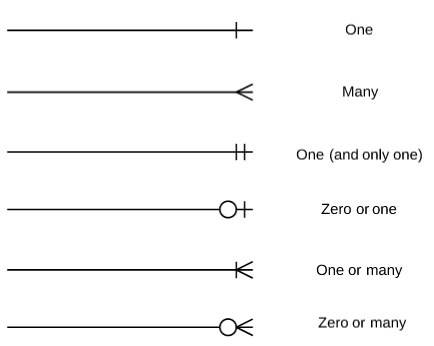
\includegraphics{./screenshots/ER-diagram-symbols.png}

The \texttt{information\_schema} is a trove of information \emph{about}
the database. Its format is more or less consistent across the different
SQL implementations that are available. Here we explore some of what's
available using several different methods. Postgres stores
\href{https://www.postgresql.org/docs/current/static/infoschema-columns.html}{a
lot of metadata}.

\hypertarget{contents-of-the-information_schema}{%
\subsection{\texorpdfstring{Contents of the
\texttt{information\_schema}}{Contents of the information\_schema}}\label{contents-of-the-information_schema}}

For this chapter R needs the \texttt{dbplyr} package to access alternate
schemas. A
\href{http://www.postgresqltutorial.com/postgresql-server-and-database-objects/}{schema}
is an object that contains one or more tables. Most often there will be
a default schema, but to access the metadata, you need to explicitly
specify which schema contains the data you want.

\hypertarget{what-tables-are-in-the-database}{%
\subsection{What tables are in the
database?}\label{what-tables-are-in-the-database}}

The simplest way to get a list of tables is with

\begin{Shaded}
\begin{Highlighting}[]
\NormalTok{table_list  <-}\StringTok{ }\NormalTok{DBI}\OperatorTok{::}\KeywordTok{dbListTables}\NormalTok{(con)}

\KeywordTok{kable}\NormalTok{(table_list)}
\end{Highlighting}
\end{Shaded}

\begin{tabular}{l}
\hline
x\\
\hline
actor\_info\\
\hline
customer\_list\\
\hline
film\_list\\
\hline
nicer\_but\_slower\_film\_list\\
\hline
sales\_by\_film\_category\\
\hline
staff\\
\hline
sales\_by\_store\\
\hline
staff\_list\\
\hline
category\\
\hline
film\_category\\
\hline
country\\
\hline
actor\\
\hline
language\\
\hline
inventory\\
\hline
payment\\
\hline
rental\\
\hline
city\\
\hline
store\\
\hline
film\\
\hline
address\\
\hline
film\_actor\\
\hline
customer\\
\hline
\end{tabular}

\hypertarget{digging-into-the-information_schema}{%
\subsection{\texorpdfstring{Digging into the
\texttt{information\_schema}}{Digging into the information\_schema}}\label{digging-into-the-information_schema}}

We usually need more detail than just a list of tables. Most SQL
databases have an \texttt{information\_schema} that has a standard
structure to describe and control the database.

The \texttt{information\_schema} is in a different schema from the
default, so to connect to the \texttt{tables} table in the
\texttt{information\_schema} we connect to the database in a different
way:

\begin{Shaded}
\begin{Highlighting}[]
\NormalTok{table_info_schema_table <-}\StringTok{ }\KeywordTok{tbl}\NormalTok{(con, dbplyr}\OperatorTok{::}\KeywordTok{in_schema}\NormalTok{(}\StringTok{"information_schema"}\NormalTok{, }\StringTok{"tables"}\NormalTok{))}
\end{Highlighting}
\end{Shaded}

The \texttt{information\_schema} is large and complex and contains 210
tables. So it's easy to get lost in it.

This query retrieves a list of the tables in the database that includes
additional detail, not just the name of the table.

\begin{Shaded}
\begin{Highlighting}[]
\NormalTok{table_info <-}\StringTok{ }\NormalTok{table_info_schema_table }\OperatorTok
\StringTok{  }\KeywordTok{filter}\NormalTok{(table_schema }\OperatorTok{==}\StringTok{ "public"}\NormalTok{) }\OperatorTok
\StringTok{  }\KeywordTok{select}\NormalTok{(table_catalog, table_schema, table_name, table_type) }\OperatorTok
\StringTok{  }\KeywordTok{arrange}\NormalTok{(table_type, table_name) }\OperatorTok\StringTok{ }
\StringTok{  }\KeywordTok{collect}\NormalTok{() }

\KeywordTok{kable}\NormalTok{(table_info)}
\end{Highlighting}
\end{Shaded}

\begin{tabular}{l|l|l|l}
\hline
table\_catalog & table\_schema & table\_name & table\_type\\
\hline
dvdrental & public & actor & BASE TABLE\\
\hline
dvdrental & public & address & BASE TABLE\\
\hline
dvdrental & public & category & BASE TABLE\\
\hline
dvdrental & public & city & BASE TABLE\\
\hline
dvdrental & public & country & BASE TABLE\\
\hline
dvdrental & public & customer & BASE TABLE\\
\hline
dvdrental & public & film & BASE TABLE\\
\hline
dvdrental & public & film\_actor & BASE TABLE\\
\hline
dvdrental & public & film\_category & BASE TABLE\\
\hline
dvdrental & public & inventory & BASE TABLE\\
\hline
dvdrental & public & language & BASE TABLE\\
\hline
dvdrental & public & payment & BASE TABLE\\
\hline
dvdrental & public & rental & BASE TABLE\\
\hline
dvdrental & public & staff & BASE TABLE\\
\hline
dvdrental & public & store & BASE TABLE\\
\hline
dvdrental & public & actor\_info & VIEW\\
\hline
dvdrental & public & customer\_list & VIEW\\
\hline
dvdrental & public & film\_list & VIEW\\
\hline
dvdrental & public & nicer\_but\_slower\_film\_list & VIEW\\
\hline
dvdrental & public & sales\_by\_film\_category & VIEW\\
\hline
dvdrental & public & sales\_by\_store & VIEW\\
\hline
dvdrental & public & staff\_list & VIEW\\
\hline
\end{tabular}

In this context \texttt{table\_catalog} is synonymous with
\texttt{database}.

Notice that \emph{VIEWS} are composites made up of one or more
\emph{BASE TABLES}.

The SQL world has its own terminology. For example \texttt{rs} is
shorthand for \texttt{result\ set}. That's equivalent to using
\texttt{df} for a \texttt{data\ frame}. The following SQL query returns
the same information as the previous one.

\begin{Shaded}
\begin{Highlighting}[]
\NormalTok{rs <-}\StringTok{ }\KeywordTok{dbGetQuery}\NormalTok{(}
\NormalTok{  con,}
  \StringTok{"select table_catalog, table_schema, table_name, table_type }
\StringTok{  from information_schema.tables }
\StringTok{  where table_schema not in ('pg_catalog','information_schema')}
\StringTok{  order by table_type, table_name }
\StringTok{  ;"}
\NormalTok{)}
\KeywordTok{kable}\NormalTok{(rs)}
\end{Highlighting}
\end{Shaded}

\begin{tabular}{l|l|l|l}
\hline
table\_catalog & table\_schema & table\_name & table\_type\\
\hline
dvdrental & public & actor & BASE TABLE\\
\hline
dvdrental & public & address & BASE TABLE\\
\hline
dvdrental & public & category & BASE TABLE\\
\hline
dvdrental & public & city & BASE TABLE\\
\hline
dvdrental & public & country & BASE TABLE\\
\hline
dvdrental & public & customer & BASE TABLE\\
\hline
dvdrental & public & film & BASE TABLE\\
\hline
dvdrental & public & film\_actor & BASE TABLE\\
\hline
dvdrental & public & film\_category & BASE TABLE\\
\hline
dvdrental & public & inventory & BASE TABLE\\
\hline
dvdrental & public & language & BASE TABLE\\
\hline
dvdrental & public & payment & BASE TABLE\\
\hline
dvdrental & public & rental & BASE TABLE\\
\hline
dvdrental & public & staff & BASE TABLE\\
\hline
dvdrental & public & store & BASE TABLE\\
\hline
dvdrental & public & actor\_info & VIEW\\
\hline
dvdrental & public & customer\_list & VIEW\\
\hline
dvdrental & public & film\_list & VIEW\\
\hline
dvdrental & public & nicer\_but\_slower\_film\_list & VIEW\\
\hline
dvdrental & public & sales\_by\_film\_category & VIEW\\
\hline
dvdrental & public & sales\_by\_store & VIEW\\
\hline
dvdrental & public & staff\_list & VIEW\\
\hline
\end{tabular}

\hypertarget{what-columns-do-those-tables-contain}{%
\section{What columns do those tables
contain?}\label{what-columns-do-those-tables-contain}}

Of course, the \texttt{DBI} package has a \texttt{dbListFields} function
that provides the simplest way to get the minimum, a list of column
names:

\begin{Shaded}
\begin{Highlighting}[]
\NormalTok{DBI}\OperatorTok{::}\KeywordTok{dbListFields}\NormalTok{(con, }\StringTok{"rental"}\NormalTok{)}
\end{Highlighting}
\end{Shaded}

\begin{verbatim}
## [1] "rental_id"    "rental_date"  "inventory_id" "customer_id" 
## [5] "return_date"  "staff_id"     "last_update"
\end{verbatim}

But the \texttt{information\_schema} has a lot more useful information
that we can use.

\begin{Shaded}
\begin{Highlighting}[]
\NormalTok{columns_info_schema_table <-}\StringTok{ }\KeywordTok{tbl}\NormalTok{(con, dbplyr}\OperatorTok{::}\KeywordTok{in_schema}\NormalTok{(}\StringTok{"information_schema"}\NormalTok{, }\StringTok{"columns"}\NormalTok{))}
\end{Highlighting}
\end{Shaded}

Since the \texttt{information\_schema} contains 1855 columns, we are
narrowing our focus to just one table. This query retrieves more
information about the \texttt{rental} table:

\begin{Shaded}
\begin{Highlighting}[]
\NormalTok{columns_info_schema_info <-}\StringTok{ }\NormalTok{columns_info_schema_table }\OperatorTok
\StringTok{  }\KeywordTok{filter}\NormalTok{(table_schema }\OperatorTok{==}\StringTok{ "public"}\NormalTok{) }\OperatorTok\StringTok{ }
\StringTok{  }\KeywordTok{select}\NormalTok{(}
\NormalTok{    table_catalog, table_schema, table_name, column_name, data_type, ordinal_position,}
\NormalTok{    character_maximum_length, column_default, numeric_precision, numeric_precision_radix}
\NormalTok{  ) }\OperatorTok
\StringTok{  }\KeywordTok{collect}\NormalTok{(}\DataTypeTok{n =} \OtherTok{Inf}\NormalTok{) }\OperatorTok\StringTok{ }
\StringTok{  }\KeywordTok{mutate}\NormalTok{(}\DataTypeTok{data_type =} \KeywordTok{case_when}\NormalTok{(}
\NormalTok{           data_type }\OperatorTok{==}\StringTok{ "character varying"} \OperatorTok{~}\StringTok{ }\KeywordTok{paste0}\NormalTok{(data_type, }\StringTok{' ('}\NormalTok{, character_maximum_length, }\StringTok{')'}\NormalTok{),}
\NormalTok{           data_type }\OperatorTok{==}\StringTok{ "real"} \OperatorTok{~}\StringTok{ }\KeywordTok{paste0}\NormalTok{(data_type, }\StringTok{' ('}\NormalTok{, numeric_precision, }\StringTok{','}\NormalTok{, numeric_precision_radix,}\StringTok{')'}\NormalTok{),}
           \OtherTok{TRUE} \OperatorTok{~}\StringTok{ }\NormalTok{data_type)}
\NormalTok{         ) }\OperatorTok\StringTok{ }
\StringTok{  }\KeywordTok{filter}\NormalTok{(table_name }\OperatorTok{==}\StringTok{ "rental"}\NormalTok{) }\OperatorTok
\StringTok{  }\KeywordTok{select}\NormalTok{(}\OperatorTok{-}\NormalTok{table_schema, }\OperatorTok{-}\NormalTok{numeric_precision, }\OperatorTok{-}\NormalTok{numeric_precision_radix)}

\KeywordTok{glimpse}\NormalTok{(columns_info_schema_info)}
\end{Highlighting}
\end{Shaded}

\begin{verbatim}
## Observations: 7
## Variables: 7
## $ table_catalog            <chr> "dvdrental", "dvdrental", "dvdrental"...
## $ table_name               <chr> "rental", "rental", "rental", "rental...
## $ column_name              <chr> "rental_id", "rental_date", "inventor...
## $ data_type                <chr> "integer", "timestamp without time zo...
## $ ordinal_position         <int> 1, 2, 3, 4, 5, 6, 7
## $ character_maximum_length <int> NA, NA, NA, NA, NA, NA, NA
## $ column_default           <chr> "nextval('rental_rental_id_seq'::regc...
\end{verbatim}

\begin{Shaded}
\begin{Highlighting}[]
\KeywordTok{kable}\NormalTok{(columns_info_schema_info)}
\end{Highlighting}
\end{Shaded}

\begin{tabular}{l|l|l|l|r|r|l}
\hline
table\_catalog & table\_name & column\_name & data\_type & ordinal\_position & character\_maximum\_length & column\_default\\
\hline
dvdrental & rental & rental\_id & integer & 1 & NA & nextval('rental\_rental\_id\_seq'::regclass)\\
\hline
dvdrental & rental & rental\_date & timestamp without time zone & 2 & NA & NA\\
\hline
dvdrental & rental & inventory\_id & integer & 3 & NA & NA\\
\hline
dvdrental & rental & customer\_id & smallint & 4 & NA & NA\\
\hline
dvdrental & rental & return\_date & timestamp without time zone & 5 & NA & NA\\
\hline
dvdrental & rental & staff\_id & smallint & 6 & NA & NA\\
\hline
dvdrental & rental & last\_update & timestamp without time zone & 7 & NA & now()\\
\hline
\end{tabular}

\hypertarget{what-is-the-difference-between-a-view-and-a-base-table}{%
\subsection{\texorpdfstring{What is the difference between a
\texttt{VIEW} and a
\texttt{BASE\ TABLE}?}{What is the difference between a VIEW and a BASE TABLE?}}\label{what-is-the-difference-between-a-view-and-a-base-table}}

The \texttt{BASE\ TABLE} has the underlying data in the database

\begin{Shaded}
\begin{Highlighting}[]
\NormalTok{table_info_schema_table }\OperatorTok
\StringTok{  }\KeywordTok{filter}\NormalTok{(table_schema }\OperatorTok{==}\StringTok{ "public"} \OperatorTok{&}\StringTok{ }\NormalTok{table_type }\OperatorTok{==}\StringTok{ "BASE TABLE"}\NormalTok{) }\OperatorTok\StringTok{ }
\StringTok{  }\KeywordTok{select}\NormalTok{(table_name, table_type) }\OperatorTok\StringTok{ }
\StringTok{  }\KeywordTok{left_join}\NormalTok{(columns_info_schema_table, }\DataTypeTok{by =} \KeywordTok{c}\NormalTok{(}\StringTok{"table_name"}\NormalTok{ =}\StringTok{ "table_name"}\NormalTok{)) }\OperatorTok\StringTok{ }
\StringTok{  }\KeywordTok{select}\NormalTok{(}
\NormalTok{    table_type, table_name, column_name, data_type, ordinal_position,}
\NormalTok{    column_default}
\NormalTok{  ) }\OperatorTok
\StringTok{  }\KeywordTok{collect}\NormalTok{(}\DataTypeTok{n =} \OtherTok{Inf}\NormalTok{) }\OperatorTok\StringTok{ }
\StringTok{  }\KeywordTok{filter}\NormalTok{(}\KeywordTok{str_detect}\NormalTok{(table_name, }\StringTok{"cust"}\NormalTok{)) }\OperatorTok\StringTok{ }
\StringTok{  }\KeywordTok{kable}\NormalTok{()}
\end{Highlighting}
\end{Shaded}

\begin{tabular}{l|l|l|l|r|l}
\hline
table\_type & table\_name & column\_name & data\_type & ordinal\_position & column\_default\\
\hline
BASE TABLE & customer & store\_id & smallint & 2 & NA\\
\hline
BASE TABLE & customer & first\_name & character varying & 3 & NA\\
\hline
BASE TABLE & customer & last\_name & character varying & 4 & NA\\
\hline
BASE TABLE & customer & email & character varying & 5 & NA\\
\hline
BASE TABLE & customer & address\_id & smallint & 6 & NA\\
\hline
BASE TABLE & customer & active & integer & 10 & NA\\
\hline
BASE TABLE & customer & customer\_id & integer & 1 & nextval('customer\_customer\_id\_seq'::regclass)\\
\hline
BASE TABLE & customer & activebool & boolean & 7 & true\\
\hline
BASE TABLE & customer & create\_date & date & 8 & ('now'::text)::date\\
\hline
BASE TABLE & customer & last\_update & timestamp without time zone & 9 & now()\\
\hline
\end{tabular}

Probably should explore how the \texttt{VIEW} is made up of data from
BASE TABLEs.

\begin{Shaded}
\begin{Highlighting}[]
\NormalTok{table_info_schema_table }\OperatorTok
\StringTok{  }\KeywordTok{filter}\NormalTok{(table_schema }\OperatorTok{==}\StringTok{ "public"} \OperatorTok{&}\StringTok{ }\NormalTok{table_type }\OperatorTok{==}\StringTok{ "VIEW"}\NormalTok{) }\OperatorTok\StringTok{  }
\StringTok{  }\KeywordTok{select}\NormalTok{(table_name, table_type) }\OperatorTok\StringTok{ }
\StringTok{  }\KeywordTok{left_join}\NormalTok{(columns_info_schema_table, }\DataTypeTok{by =} \KeywordTok{c}\NormalTok{(}\StringTok{"table_name"}\NormalTok{ =}\StringTok{ "table_name"}\NormalTok{)) }\OperatorTok\StringTok{ }
\StringTok{  }\KeywordTok{select}\NormalTok{(}
\NormalTok{    table_type, table_name, column_name, data_type, ordinal_position,}
\NormalTok{    column_default}
\NormalTok{  ) }\OperatorTok
\StringTok{  }\KeywordTok{collect}\NormalTok{(}\DataTypeTok{n =} \OtherTok{Inf}\NormalTok{) }\OperatorTok\StringTok{ }
\StringTok{  }\KeywordTok{filter}\NormalTok{(}\KeywordTok{str_detect}\NormalTok{(table_name, }\StringTok{"cust"}\NormalTok{)) }\OperatorTok\StringTok{ }
\StringTok{  }\KeywordTok{kable}\NormalTok{()}
\end{Highlighting}
\end{Shaded}

\begin{tabular}{l|l|l|l|r|l}
\hline
table\_type & table\_name & column\_name & data\_type & ordinal\_position & column\_default\\
\hline
VIEW & customer\_list & id & integer & 1 & NA\\
\hline
VIEW & customer\_list & name & text & 2 & NA\\
\hline
VIEW & customer\_list & address & character varying & 3 & NA\\
\hline
VIEW & customer\_list & zip code & character varying & 4 & NA\\
\hline
VIEW & customer\_list & phone & character varying & 5 & NA\\
\hline
VIEW & customer\_list & city & character varying & 6 & NA\\
\hline
VIEW & customer\_list & country & character varying & 7 & NA\\
\hline
VIEW & customer\_list & notes & text & 8 & NA\\
\hline
VIEW & customer\_list & sid & smallint & 9 & NA\\
\hline
\end{tabular}

\hypertarget{what-data-types-are-found-in-the-database}{%
\subsection{What data types are found in the
database?}\label{what-data-types-are-found-in-the-database}}

\begin{Shaded}
\begin{Highlighting}[]
\NormalTok{columns_info_schema_info }\OperatorTok\StringTok{ }\KeywordTok{count}\NormalTok{(data_type)}
\end{Highlighting}
\end{Shaded}

\begin{verbatim}
## # A tibble: 3 x 2
##   data_type                       n
##   <chr>                       <int>
## 1 integer                         2
## 2 smallint                        2
## 3 timestamp without time zone     3
\end{verbatim}

\hypertarget{characterizing-how-things-are-named}{%
\section{Characterizing how things are
named}\label{characterizing-how-things-are-named}}

Names are the handle for accessing the data. Tables and columns may or
may not be named consistently or in a way that makes sense to you. You
should look at these names \emph{as data}.

\hypertarget{counting-columns-and-name-reuse}{%
\subsection{Counting columns and name
reuse}\label{counting-columns-and-name-reuse}}

Pull out some rough-and-ready but useful statistics about your database.
Since we are in SQL-land we talk about variables as \texttt{columns}.

\begin{Shaded}
\begin{Highlighting}[]
\NormalTok{public_tables <-}\StringTok{ }\NormalTok{columns_info_schema_table }\OperatorTok
\StringTok{  }\KeywordTok{filter}\NormalTok{(table_schema }\OperatorTok{==}\StringTok{ "public"}\NormalTok{) }\OperatorTok\StringTok{ }
\StringTok{  }\KeywordTok{collect}\NormalTok{()}

\NormalTok{public_tables }\OperatorTok\StringTok{ }\KeywordTok{count}\NormalTok{(table_name, }\DataTypeTok{sort =} \OtherTok{TRUE}\NormalTok{) }\OperatorTok\StringTok{ }
\StringTok{  }\KeywordTok{kable}\NormalTok{()}
\end{Highlighting}
\end{Shaded}

\begin{tabular}{l|r}
\hline
table\_name & n\\
\hline
film & 13\\
\hline
staff & 11\\
\hline
customer & 10\\
\hline
customer\_list & 9\\
\hline
address & 8\\
\hline
film\_list & 8\\
\hline
nicer\_but\_slower\_film\_list & 8\\
\hline
staff\_list & 8\\
\hline
rental & 7\\
\hline
payment & 6\\
\hline
actor & 4\\
\hline
actor\_info & 4\\
\hline
city & 4\\
\hline
inventory & 4\\
\hline
store & 4\\
\hline
category & 3\\
\hline
country & 3\\
\hline
film\_actor & 3\\
\hline
film\_category & 3\\
\hline
language & 3\\
\hline
sales\_by\_store & 3\\
\hline
sales\_by\_film\_category & 2\\
\hline
\end{tabular}

How many \emph{column names} are shared across tables (or duplicated)?

\begin{Shaded}
\begin{Highlighting}[]
\NormalTok{public_tables }\OperatorTok\StringTok{ }\KeywordTok{count}\NormalTok{(column_name, }\DataTypeTok{sort =} \OtherTok{TRUE}\NormalTok{) }\OperatorTok\StringTok{ }\KeywordTok{filter}\NormalTok{(n }\OperatorTok{>}\StringTok{ }\DecValTok{1}\NormalTok{)}
\end{Highlighting}
\end{Shaded}

\begin{verbatim}
## # A tibble: 34 x 2
##    column_name     n
##    <chr>       <int>
##  1 last_update    14
##  2 address_id      4
##  3 film_id         4
##  4 first_name      4
##  5 last_name       4
##  6 name            4
##  7 store_id        4
##  8 actor_id        3
##  9 address         3
## 10 category        3
## # ... with 24 more rows
\end{verbatim}

How many column names are unique?

\begin{Shaded}
\begin{Highlighting}[]
\NormalTok{public_tables }\OperatorTok\StringTok{ }\KeywordTok{count}\NormalTok{(column_name) }\OperatorTok\StringTok{ }\KeywordTok{filter}\NormalTok{(n }\OperatorTok{==}\StringTok{ }\DecValTok{1}\NormalTok{) }\OperatorTok\StringTok{ }\KeywordTok{count}\NormalTok{()}
\end{Highlighting}
\end{Shaded}

\begin{verbatim}
## # A tibble: 1 x 1
##      nn
##   <int>
## 1    24
\end{verbatim}

\hypertarget{database-keys}{%
\section{Database keys}\label{database-keys}}

\hypertarget{direct-sql}{%
\subsection{Direct SQL}\label{direct-sql}}

How do we use this output? Could it be generated by dplyr?

\begin{Shaded}
\begin{Highlighting}[]
\NormalTok{rs <-}\StringTok{ }\KeywordTok{dbGetQuery}\NormalTok{(}
\NormalTok{  con,}
  \StringTok{"}
\StringTok{--SELECT conrelid::regclass as table_from}
\StringTok{select table_catalog||'.'||table_schema||'.'||table_name table_name}
\StringTok{, conname, pg_catalog.pg_get_constraintdef(r.oid, true) as condef}
\StringTok{FROM information_schema.columns c,pg_catalog.pg_constraint r}
\StringTok{WHERE 1 = 1 --r.conrelid = '16485' }
\StringTok{  AND r.contype  in ('f','p') ORDER BY 1}
\StringTok{;"}
\NormalTok{)}
\KeywordTok{glimpse}\NormalTok{(rs)}
\end{Highlighting}
\end{Shaded}

\begin{verbatim}
## Observations: 61,215
## Variables: 3
## $ table_name <chr> "dvdrental.information_schema.administrable_role_au...
## $ conname    <chr> "actor_pkey", "actor_pkey", "actor_pkey", "country_...
## $ condef     <chr> "PRIMARY KEY (actor_id)", "PRIMARY KEY (actor_id)",...
\end{verbatim}

\begin{Shaded}
\begin{Highlighting}[]
\KeywordTok{kable}\NormalTok{(}\KeywordTok{head}\NormalTok{(rs))}
\end{Highlighting}
\end{Shaded}

\begin{tabular}{l|l|l}
\hline
table\_name & conname & condef\\
\hline
dvdrental.information\_schema.administrable\_role\_authorizations & actor\_pkey & PRIMARY KEY (actor\_id)\\
\hline
dvdrental.information\_schema.administrable\_role\_authorizations & actor\_pkey & PRIMARY KEY (actor\_id)\\
\hline
dvdrental.information\_schema.administrable\_role\_authorizations & actor\_pkey & PRIMARY KEY (actor\_id)\\
\hline
dvdrental.information\_schema.administrable\_role\_authorizations & country\_pkey & PRIMARY KEY (country\_id)\\
\hline
dvdrental.information\_schema.administrable\_role\_authorizations & country\_pkey & PRIMARY KEY (country\_id)\\
\hline
dvdrental.information\_schema.administrable\_role\_authorizations & country\_pkey & PRIMARY KEY (country\_id)\\
\hline
\end{tabular}

The following is more compact and looks more useful. What is the
difference between the two?

\begin{Shaded}
\begin{Highlighting}[]
\NormalTok{rs <-}\StringTok{ }\KeywordTok{dbGetQuery}\NormalTok{(}
\NormalTok{  con,}
  \StringTok{"select conrelid::regclass as table_from}
\StringTok{      ,c.conname}
\StringTok{      ,pg_get_constraintdef(c.oid)}
\StringTok{  from pg_constraint c}
\StringTok{  join pg_namespace n on n.oid = c.connamespace}
\StringTok{ where c.contype in ('f','p')}
\StringTok{   and n.nspname = 'public'}
\StringTok{order by conrelid::regclass::text, contype DESC;}
\StringTok{"}
\NormalTok{)}
\KeywordTok{glimpse}\NormalTok{(rs)}
\end{Highlighting}
\end{Shaded}

\begin{verbatim}
## Observations: 33
## Variables: 3
## $ table_from           <chr> "actor", "address", "address", "category"...
## $ conname              <chr> "actor_pkey", "address_pkey", "fk_address...
## $ pg_get_constraintdef <chr> "PRIMARY KEY (actor_id)", "PRIMARY KEY (a...
\end{verbatim}

\begin{Shaded}
\begin{Highlighting}[]
\KeywordTok{kable}\NormalTok{(}\KeywordTok{head}\NormalTok{(rs))}
\end{Highlighting}
\end{Shaded}

\begin{tabular}{l|l|l}
\hline
table\_from & conname & pg\_get\_constraintdef\\
\hline
actor & actor\_pkey & PRIMARY KEY (actor\_id)\\
\hline
address & address\_pkey & PRIMARY KEY (address\_id)\\
\hline
address & fk\_address\_city & FOREIGN KEY (city\_id) REFERENCES city(city\_id)\\
\hline
category & category\_pkey & PRIMARY KEY (category\_id)\\
\hline
city & city\_pkey & PRIMARY KEY (city\_id)\\
\hline
city & fk\_city & FOREIGN KEY (country\_id) REFERENCES country(country\_id)\\
\hline
\end{tabular}

\begin{Shaded}
\begin{Highlighting}[]
\KeywordTok{dim}\NormalTok{(rs)[}\DecValTok{1}\NormalTok{]}
\end{Highlighting}
\end{Shaded}

\begin{verbatim}
## [1] 33
\end{verbatim}

\hypertarget{database-keys-with-dplyr}{%
\subsection{Database keys with dplyr}\label{database-keys-with-dplyr}}

This query shows the primary and foreign keys in the database.

\begin{Shaded}
\begin{Highlighting}[]
\NormalTok{tables <-}\StringTok{ }\KeywordTok{tbl}\NormalTok{(con, dbplyr}\OperatorTok{::}\KeywordTok{in_schema}\NormalTok{(}\StringTok{"information_schema"}\NormalTok{, }\StringTok{"tables"}\NormalTok{))}
\NormalTok{table_constraints <-}\StringTok{ }\KeywordTok{tbl}\NormalTok{(con, dbplyr}\OperatorTok{::}\KeywordTok{in_schema}\NormalTok{(}\StringTok{"information_schema"}\NormalTok{, }\StringTok{"table_constraints"}\NormalTok{))}
\NormalTok{key_column_usage <-}\StringTok{ }\KeywordTok{tbl}\NormalTok{(con, dbplyr}\OperatorTok{::}\KeywordTok{in_schema}\NormalTok{(}\StringTok{"information_schema"}\NormalTok{, }\StringTok{"key_column_usage"}\NormalTok{))}
\NormalTok{referential_constraints <-}\StringTok{ }\KeywordTok{tbl}\NormalTok{(con, dbplyr}\OperatorTok{::}\KeywordTok{in_schema}\NormalTok{(}\StringTok{"information_schema"}\NormalTok{, }\StringTok{"referential_constraints"}\NormalTok{))}
\NormalTok{constraint_column_usage <-}\StringTok{ }\KeywordTok{tbl}\NormalTok{(con, dbplyr}\OperatorTok{::}\KeywordTok{in_schema}\NormalTok{(}\StringTok{"information_schema"}\NormalTok{, }\StringTok{"constraint_column_usage"}\NormalTok{))}

\NormalTok{keys <-}\StringTok{ }\NormalTok{tables }\OperatorTok\StringTok{ }
\StringTok{  }\KeywordTok{left_join}\NormalTok{(table_constraints, }\DataTypeTok{by =} \KeywordTok{c}\NormalTok{(}
    \StringTok{"table_catalog"}\NormalTok{ =}\StringTok{ "table_catalog"}\NormalTok{,}
    \StringTok{"table_schema"}\NormalTok{ =}\StringTok{  "table_schema"}\NormalTok{,}
    \StringTok{"table_name"}\NormalTok{ =}\StringTok{ "table_name"}
\NormalTok{  )) }\OperatorTok\StringTok{ }
\StringTok{  }\CommentTok{# table_constraints %>% }
\StringTok{  }\KeywordTok{filter}\NormalTok{(constraint_type }\OperatorTok\StringTok{ }\KeywordTok{c}\NormalTok{(}\StringTok{"FOREIGN KEY"}\NormalTok{, }\StringTok{"PRIMARY KEY"}\NormalTok{)) }\OperatorTok\StringTok{ }
\StringTok{  }\KeywordTok{left_join}\NormalTok{(key_column_usage, }
            \DataTypeTok{by =} \KeywordTok{c}\NormalTok{(}
              \StringTok{"table_catalog"}\NormalTok{ =}\StringTok{ "table_catalog"}\NormalTok{,}
              \StringTok{"constraint_catalog"}\NormalTok{ =}\StringTok{ "constraint_catalog"}\NormalTok{,}
              \StringTok{"constraint_schema"}\NormalTok{ =}\StringTok{ "constraint_schema"}\NormalTok{,}
              \StringTok{"table_name"}\NormalTok{ =}\StringTok{ "table_name"}\NormalTok{,}
              \StringTok{"table_schema"}\NormalTok{ =}\StringTok{ "table_schema"}\NormalTok{,}
              \StringTok{"constraint_name"}\NormalTok{ =}\StringTok{ "constraint_name"}
\NormalTok{              )) }\OperatorTok
\StringTok{  }\CommentTok{# left_join(constraint_column_usage) %>% # does this table add anything useful?}
\StringTok{  }\KeywordTok{select}\NormalTok{(table_name, table_type, constraint_name, constraint_type, column_name, ordinal_position) }\OperatorTok
\StringTok{  }\KeywordTok{arrange}\NormalTok{(table_name) }\OperatorTok\StringTok{ }
\KeywordTok{collect}\NormalTok{()}
\KeywordTok{glimpse}\NormalTok{(keys)}
\end{Highlighting}
\end{Shaded}

\begin{verbatim}
## Observations: 35
## Variables: 6
## $ table_name       <chr> "actor", "address", "address", "category", "c...
## $ table_type       <chr> "BASE TABLE", "BASE TABLE", "BASE TABLE", "BA...
## $ constraint_name  <chr> "actor_pkey", "address_pkey", "fk_address_cit...
## $ constraint_type  <chr> "PRIMARY KEY", "PRIMARY KEY", "FOREIGN KEY", ...
## $ column_name      <chr> "actor_id", "address_id", "city_id", "categor...
## $ ordinal_position <int> 1, 1, 1, 1, 1, 1, 1, 1, 1, 1, 1, 1, 1, 1, 2, ...
\end{verbatim}

\begin{Shaded}
\begin{Highlighting}[]
\KeywordTok{kable}\NormalTok{(keys)}
\end{Highlighting}
\end{Shaded}

\begin{tabular}{l|l|l|l|l|r}
\hline
table\_name & table\_type & constraint\_name & constraint\_type & column\_name & ordinal\_position\\
\hline
actor & BASE TABLE & actor\_pkey & PRIMARY KEY & actor\_id & 1\\
\hline
address & BASE TABLE & address\_pkey & PRIMARY KEY & address\_id & 1\\
\hline
address & BASE TABLE & fk\_address\_city & FOREIGN KEY & city\_id & 1\\
\hline
category & BASE TABLE & category\_pkey & PRIMARY KEY & category\_id & 1\\
\hline
city & BASE TABLE & city\_pkey & PRIMARY KEY & city\_id & 1\\
\hline
city & BASE TABLE & fk\_city & FOREIGN KEY & country\_id & 1\\
\hline
country & BASE TABLE & country\_pkey & PRIMARY KEY & country\_id & 1\\
\hline
customer & BASE TABLE & customer\_address\_id\_fkey & FOREIGN KEY & address\_id & 1\\
\hline
customer & BASE TABLE & customer\_pkey & PRIMARY KEY & customer\_id & 1\\
\hline
film & BASE TABLE & film\_language\_id\_fkey & FOREIGN KEY & language\_id & 1\\
\hline
film & BASE TABLE & film\_pkey & PRIMARY KEY & film\_id & 1\\
\hline
film\_actor & BASE TABLE & film\_actor\_actor\_id\_fkey & FOREIGN KEY & actor\_id & 1\\
\hline
film\_actor & BASE TABLE & film\_actor\_film\_id\_fkey & FOREIGN KEY & film\_id & 1\\
\hline
film\_actor & BASE TABLE & film\_actor\_pkey & PRIMARY KEY & actor\_id & 1\\
\hline
film\_actor & BASE TABLE & film\_actor\_pkey & PRIMARY KEY & film\_id & 2\\
\hline
film\_category & BASE TABLE & film\_category\_category\_id\_fkey & FOREIGN KEY & category\_id & 1\\
\hline
film\_category & BASE TABLE & film\_category\_film\_id\_fkey & FOREIGN KEY & film\_id & 1\\
\hline
film\_category & BASE TABLE & film\_category\_pkey & PRIMARY KEY & film\_id & 1\\
\hline
film\_category & BASE TABLE & film\_category\_pkey & PRIMARY KEY & category\_id & 2\\
\hline
inventory & BASE TABLE & inventory\_film\_id\_fkey & FOREIGN KEY & film\_id & 1\\
\hline
inventory & BASE TABLE & inventory\_pkey & PRIMARY KEY & inventory\_id & 1\\
\hline
language & BASE TABLE & language\_pkey & PRIMARY KEY & language\_id & 1\\
\hline
payment & BASE TABLE & payment\_customer\_id\_fkey & FOREIGN KEY & customer\_id & 1\\
\hline
payment & BASE TABLE & payment\_pkey & PRIMARY KEY & payment\_id & 1\\
\hline
payment & BASE TABLE & payment\_rental\_id\_fkey & FOREIGN KEY & rental\_id & 1\\
\hline
payment & BASE TABLE & payment\_staff\_id\_fkey & FOREIGN KEY & staff\_id & 1\\
\hline
rental & BASE TABLE & rental\_customer\_id\_fkey & FOREIGN KEY & customer\_id & 1\\
\hline
rental & BASE TABLE & rental\_inventory\_id\_fkey & FOREIGN KEY & inventory\_id & 1\\
\hline
rental & BASE TABLE & rental\_pkey & PRIMARY KEY & rental\_id & 1\\
\hline
rental & BASE TABLE & rental\_staff\_id\_key & FOREIGN KEY & staff\_id & 1\\
\hline
staff & BASE TABLE & staff\_address\_id\_fkey & FOREIGN KEY & address\_id & 1\\
\hline
staff & BASE TABLE & staff\_pkey & PRIMARY KEY & staff\_id & 1\\
\hline
store & BASE TABLE & store\_address\_id\_fkey & FOREIGN KEY & address\_id & 1\\
\hline
store & BASE TABLE & store\_manager\_staff\_id\_fkey & FOREIGN KEY & manager\_staff\_id & 1\\
\hline
store & BASE TABLE & store\_pkey & PRIMARY KEY & store\_id & 1\\
\hline
\end{tabular}

What do we learn from the following query? How is it useful?

\begin{Shaded}
\begin{Highlighting}[]
\NormalTok{rs <-}\StringTok{ }\KeywordTok{dbGetQuery}\NormalTok{(}
\NormalTok{  con,}
  \StringTok{"SELECT r.*,}
\StringTok{  pg_catalog.pg_get_constraintdef(r.oid, true) as condef}
\StringTok{  FROM pg_catalog.pg_constraint r}
\StringTok{  WHERE 1=1 --r.conrelid = '16485' AND r.contype = 'f' ORDER BY 1;}
\StringTok{  "}
\NormalTok{  )}

\KeywordTok{head}\NormalTok{(rs)}
\end{Highlighting}
\end{Shaded}

\begin{verbatim}
##                        conname connamespace contype condeferrable
## 1 cardinal_number_domain_check        12703       c         FALSE
## 2              yes_or_no_check        12703       c         FALSE
## 3                   year_check         2200       c         FALSE
## 4                   actor_pkey         2200       p         FALSE
## 5                 address_pkey         2200       p         FALSE
## 6                category_pkey         2200       p         FALSE
##   condeferred convalidated conrelid contypid conindid confrelid
## 1       FALSE         TRUE        0    12716        0         0
## 2       FALSE         TRUE        0    12724        0         0
## 3       FALSE         TRUE        0    16397        0         0
## 4       FALSE         TRUE    16420        0    16555         0
## 5       FALSE         TRUE    16461        0    16557         0
## 6       FALSE         TRUE    16427        0    16559         0
##   confupdtype confdeltype confmatchtype conislocal coninhcount
## 1                                             TRUE           0
## 2                                             TRUE           0
## 3                                             TRUE           0
## 4                                             TRUE           0
## 5                                             TRUE           0
## 6                                             TRUE           0
##   connoinherit conkey confkey conpfeqop conppeqop conffeqop conexclop
## 1        FALSE   <NA>    <NA>      <NA>      <NA>      <NA>      <NA>
## 2        FALSE   <NA>    <NA>      <NA>      <NA>      <NA>      <NA>
## 3        FALSE   <NA>    <NA>      <NA>      <NA>      <NA>      <NA>
## 4         TRUE    {1}    <NA>      <NA>      <NA>      <NA>      <NA>
## 5         TRUE    {1}    <NA>      <NA>      <NA>      <NA>      <NA>
## 6         TRUE    {1}    <NA>      <NA>      <NA>      <NA>      <NA>
##                                                                                                                                                                                                                                                                                                                                                                                                                                                                                                                                                                                                                                                                                                                                                                                                                                                  conbin
## 1                                                                                                                                                                                                                                                                                                                                                                                                                                                                                                       {OPEXPR :opno 525 :opfuncid 150 :opresulttype 16 :opretset false :opcollid 0 :inputcollid 0 :args ({COERCETODOMAINVALUE :typeId 23 :typeMod -1 :collation 0 :location 195} {CONST :consttype 23 :consttypmod -1 :constcollid 0 :constlen 4 :constbyval true :constisnull false :location 204 :constvalue 4 [ 0 0 0 0 0 0 0 0 ]}) :location 201}
## 2 {SCALARARRAYOPEXPR :opno 98 :opfuncid 67 :useOr true :inputcollid 100 :args ({RELABELTYPE :arg {COERCETODOMAINVALUE :typeId 1043 :typeMod 7 :collation 100 :location 121} :resulttype 25 :resulttypmod -1 :resultcollid 100 :relabelformat 2 :location -1} {ARRAYCOERCEEXPR :arg {ARRAY :array_typeid 1015 :array_collid 100 :element_typeid 1043 :elements ({CONST :consttype 1043 :consttypmod -1 :constcollid 100 :constlen -1 :constbyval false :constisnull false :location 131 :constvalue 7 [ 28 0 0 0 89 69 83 ]} {CONST :consttype 1043 :consttypmod -1 :constcollid 100 :constlen -1 :constbyval false :constisnull false :location 138 :constvalue 6 [ 24 0 0 0 78 79 ]}) :multidims false :location -1} :elemfuncid 0 :resulttype 1009 :resulttypmod -1 :resultcollid 100 :isExplicit false :coerceformat 2 :location -1}) :location 127}
## 3                                                                                                             {BOOLEXPR :boolop and :args ({OPEXPR :opno 525 :opfuncid 150 :opresulttype 16 :opretset false :opcollid 0 :inputcollid 0 :args ({COERCETODOMAINVALUE :typeId 23 :typeMod -1 :collation 0 :location 62} {CONST :consttype 23 :consttypmod -1 :constcollid 0 :constlen 4 :constbyval true :constisnull false :location 71 :constvalue 4 [ 109 7 0 0 0 0 0 0 ]}) :location 68} {OPEXPR :opno 523 :opfuncid 149 :opresulttype 16 :opretset false :opcollid 0 :inputcollid 0 :args ({COERCETODOMAINVALUE :typeId 23 :typeMod -1 :collation 0 :location 82} {CONST :consttype 23 :consttypmod -1 :constcollid 0 :constlen 4 :constbyval true :constisnull false :location 91 :constvalue 4 [ 107 8 0 0 0 0 0 0 ]}) :location 88}) :location 77}
## 4                                                                                                                                                                                                                                                                                                                                                                                                                                                                                                                                                                                                                                                                                                                                                                                                                                                  <NA>
## 5                                                                                                                                                                                                                                                                                                                                                                                                                                                                                                                                                                                                                                                                                                                                                                                                                                                  <NA>
## 6                                                                                                                                                                                                                                                                                                                                                                                                                                                                                                                                                                                                                                                                                                                                                                                                                                                  <NA>
##                                                                                       consrc
## 1                                                                               (VALUE >= 0)
## 2 ((VALUE)::text = ANY ((ARRAY['YES'::character varying, 'NO'::character varying])::text[]))
## 3                                                      ((VALUE >= 1901) AND (VALUE <= 2155))
## 4                                                                                       <NA>
## 5                                                                                       <NA>
## 6                                                                                       <NA>
##                                                                                         condef
## 1                                                                           CHECK (VALUE >= 0)
## 2 CHECK (VALUE::text = ANY (ARRAY['YES'::character varying, 'NO'::character varying]::text[]))
## 3                                                      CHECK (VALUE >= 1901 AND VALUE <= 2155)
## 4                                                                       PRIMARY KEY (actor_id)
## 5                                                                     PRIMARY KEY (address_id)
## 6                                                                    PRIMARY KEY (category_id)
\end{verbatim}

\hypertarget{creating-your-own-data-dictionary}{%
\section{Creating your own data
dictionary}\label{creating-your-own-data-dictionary}}

If you are going to work with a database for an extended period it can
be useful to create your own data dictionary. Here is an illustration of
the idea

\begin{Shaded}
\begin{Highlighting}[]
\NormalTok{some_tables <-}\StringTok{ }\KeywordTok{c}\NormalTok{(}\StringTok{"rental"}\NormalTok{, }\StringTok{"city"}\NormalTok{, }\StringTok{"store"}\NormalTok{)}

\NormalTok{all_meta <-}\StringTok{ }\KeywordTok{map_df}\NormalTok{(some_tables, sp_get_dbms_data_dictionary, }\DataTypeTok{con =}\NormalTok{ con)}

\NormalTok{all_meta}
\end{Highlighting}
\end{Shaded}

\begin{verbatim}
## # A tibble: 15 x 11
##    table_name var_name var_type num_rows num_blank num_unique min   q_25 
##    <chr>      <chr>    <chr>       <int>     <int>      <int> <chr> <chr>
##  1 rental     rental_~ integer     16044         0      16044 1     4013 
##  2 rental     rental_~ double      16044         0      15815 2005~ 2005~
##  3 rental     invento~ integer     16044         0       4580 1     1154 
##  4 rental     custome~ integer     16044         0        599 1     148  
##  5 rental     return_~ double      16044       183      15836 2005~ 2005~
##  6 rental     staff_id integer     16044         0          2 1     1    
##  7 rental     last_up~ double      16044         0          3 2006~ 2006~
##  8 city       city_id  integer       600         0        600 1     150  
##  9 city       city     charact~      600         0        599 A Co~ Dzer~
## 10 city       country~ integer       600         0        109 1     28   
## 11 city       last_up~ double        600         0          1 2006~ 2006~
## 12 store      store_id integer         2         0          2 1     1    
## 13 store      manager~ integer         2         0          2 1     1    
## 14 store      address~ integer         2         0          2 1     1    
## 15 store      last_up~ double          2         0          1 2006~ 2006~
## # ... with 3 more variables: q_50 <chr>, q_75 <chr>, max <chr>
\end{verbatim}

\begin{Shaded}
\begin{Highlighting}[]
\KeywordTok{glimpse}\NormalTok{(all_meta)}
\end{Highlighting}
\end{Shaded}

\begin{verbatim}
## Observations: 15
## Variables: 11
## $ table_name <chr> "rental", "rental", "rental", "rental", "rental", "...
## $ var_name   <chr> "rental_id", "rental_date", "inventory_id", "custom...
## $ var_type   <chr> "integer", "double", "integer", "integer", "double"...
## $ num_rows   <int> 16044, 16044, 16044, 16044, 16044, 16044, 16044, 60...
## $ num_blank  <int> 0, 0, 0, 0, 183, 0, 0, 0, 0, 0, 0, 0, 0, 0, 0
## $ num_unique <int> 16044, 15815, 4580, 599, 15836, 2, 3, 600, 599, 109...
## $ min        <chr> "1", "2005-05-24 22:53:30", "1", "1", "2005-05-25 2...
## $ q_25       <chr> "4013", "2005-07-07 00:58:00", "1154", "148", "2005...
## $ q_50       <chr> "8025", "2005-07-28 16:03:27", "2291", "296", "2005...
## $ q_75       <chr> "12037", "2005-08-17 21:13:35", "3433", "446", "200...
## $ max        <chr> "16049", "2006-02-14 15:16:03", "4581", "599", "200...
\end{verbatim}

\begin{Shaded}
\begin{Highlighting}[]
\KeywordTok{kable}\NormalTok{(}\KeywordTok{head}\NormalTok{(all_meta))}
\end{Highlighting}
\end{Shaded}

\begin{tabular}{l|l|l|r|r|r|l|l|l|l|l}
\hline
table\_name & var\_name & var\_type & num\_rows & num\_blank & num\_unique & min & q\_25 & q\_50 & q\_75 & max\\
\hline
rental & rental\_id & integer & 16044 & 0 & 16044 & 1 & 4013 & 8025 & 12037 & 16049\\
\hline
rental & rental\_date & double & 16044 & 0 & 15815 & 2005-05-24 22:53:30 & 2005-07-07 00:58:00 & 2005-07-28 16:03:27 & 2005-08-17 21:13:35 & 2006-02-14 15:16:03\\
\hline
rental & inventory\_id & integer & 16044 & 0 & 4580 & 1 & 1154 & 2291 & 3433 & 4581\\
\hline
rental & customer\_id & integer & 16044 & 0 & 599 & 1 & 148 & 296 & 446 & 599\\
\hline
rental & return\_date & double & 16044 & 183 & 15836 & 2005-05-25 23:55:21 & 2005-07-10 15:48:58 & 2005-08-01 19:31:15 & 2005-08-20 23:32:29 & 2005-09-02 02:35:22\\
\hline
rental & staff\_id & integer & 16044 & 0 & 2 & 1 & 1 & 1 & 2 & 2\\
\hline
\end{tabular}

\hypertarget{save-your-work}{%
\section{Save your work!}\label{save-your-work}}

The work you do to understand the structure and contents of a database
can be useful for others (including future-you). So at the end of a
session, you might look at all the data frames you want to save.
Consider saving them in a form where you can add notes at the
appropriate level (as in a Google Doc representing table or columns that
you annotate over time).

\begin{Shaded}
\begin{Highlighting}[]
\KeywordTok{ls}\NormalTok{()}
\end{Highlighting}
\end{Shaded}

\begin{verbatim}
##  [1] "all_meta"                  "columns_info_schema_info" 
##  [3] "columns_info_schema_table" "con"                      
##  [5] "constraint_column_usage"   "cranex"                   
##  [7] "key_column_usage"          "keys"                     
##  [9] "public_tables"             "referential_constraints"  
## [11] "rental"                    "rs"                       
## [13] "some_tables"               "table_constraints"        
## [15] "table_info"                "table_info_schema_table"  
## [17] "table_list"                "tables"
\end{verbatim}

\hypertarget{drilling-into-your-db-environment-22}{%
\chapter{Drilling into Your DB Environment
(22)}\label{drilling-into-your-db-environment-22}}

Start up the \texttt{docker-pet} container

\begin{Shaded}
\begin{Highlighting}[]
\KeywordTok{sp_docker_start}\NormalTok{(}\StringTok{"sql-pet"}\NormalTok{)}
\end{Highlighting}
\end{Shaded}

Now connect to the \texttt{dvdrental} database with R

\begin{Shaded}
\begin{Highlighting}[]
\NormalTok{con <-}\StringTok{ }\KeywordTok{sp_get_postgres_connection}\NormalTok{(}
  \DataTypeTok{user =} \KeywordTok{Sys.getenv}\NormalTok{(}\StringTok{"DEFAULT_POSTGRES_USER_NAME"}\NormalTok{),}
  \DataTypeTok{password =}  \KeywordTok{Sys.getenv}\NormalTok{(}\StringTok{"DEFAULT_POSTGRES_PASSWORD"}\NormalTok{),}
  \DataTypeTok{dbname =} \StringTok{"dvdrental"}\NormalTok{,}
  \DataTypeTok{seconds_to_test =} \DecValTok{10}\NormalTok{)}
\NormalTok{con}
\end{Highlighting}
\end{Shaded}

\begin{verbatim}
## <PqConnection> dvdrental@localhost:5432
\end{verbatim}

\hypertarget{which-database}{%
\section{Which database?}\label{which-database}}

Your DBA will create your user accounts and priviledges for the
database(s) that you can access.

One of the challenges when working with a database(s) is finding where
your data actually resides. Your best resources will be one or more
subject matter experts, \texttt{SME}, and your DBA. Your data may
actually reside in multiple databases, e.g., a detail and summary
databases. In our tutorial, we focus on the one database,
\texttt{dvdrental}. Database names usually reflect something about the
data that they contain.

Your laptop is a server for the Docker Postgres databases. A database is
a collection of files that Postgres manages in the background.

\hypertarget{how-many-databases-reside-in-the-docker-container}{%
\section{How many databases reside in the Docker
Container?}\label{how-many-databases-reside-in-the-docker-container}}

\begin{Shaded}
\begin{Highlighting}[]
\NormalTok{rs <-}
\StringTok{  }\NormalTok{DBI}\OperatorTok{::}\KeywordTok{dbGetQuery}\NormalTok{(}
\NormalTok{  con,}
  \StringTok{"SELECT 'DB Names in Docker' showing}
\StringTok{          ,datname DB}
\StringTok{     FROM pg_database}
\StringTok{    WHERE datistemplate = false;}
\StringTok{  "}
\NormalTok{  )}
\KeywordTok{kable}\NormalTok{(rs)}
\end{Highlighting}
\end{Shaded}

\begin{tabular}{l|l}
\hline
showing & db\\
\hline
DB Names in Docker & postgres\\
\hline
DB Names in Docker & dvdrental\\
\hline
\end{tabular}

Which databases are available?

\begin{verbatim}
Modify the connection call to connect to the `postgres` database.
\end{verbatim}

\begin{Shaded}
\begin{Highlighting}[]
\NormalTok{con <-}\StringTok{ }\KeywordTok{sp_get_postgres_connection}\NormalTok{(}
  \DataTypeTok{user =} \KeywordTok{Sys.getenv}\NormalTok{(}\StringTok{"DEFAULT_POSTGRES_USER_NAME"}\NormalTok{),}
  \DataTypeTok{password =}  \KeywordTok{Sys.getenv}\NormalTok{(}\StringTok{"DEFAULT_POSTGRES_PASSWORD"}\NormalTok{),}
  \DataTypeTok{dbname =} \StringTok{"your code goes here"}\NormalTok{,}
  \DataTypeTok{seconds_to_test =} \DecValTok{10}\NormalTok{)}

\NormalTok{con}
\end{Highlighting}
\end{Shaded}

\begin{verbatim}
## [1] "There is no connection"
\end{verbatim}

\begin{Shaded}
\begin{Highlighting}[]
\ControlFlowTok{if}\NormalTok{ (con }\OperatorTok{!=}\StringTok{ 'There is no connection'}\NormalTok{)}
    \KeywordTok{dbDisconnect}\NormalTok{(con)}

\CommentTok{#Answer: con <PqConnection> postgres@localhost:5432}

\CommentTok{# Reconnect to dvdrental}

\NormalTok{con <-}\StringTok{ }\KeywordTok{sp_get_postgres_connection}\NormalTok{(}
  \DataTypeTok{user =} \KeywordTok{Sys.getenv}\NormalTok{(}\StringTok{"DEFAULT_POSTGRES_USER_NAME"}\NormalTok{),}
  \DataTypeTok{password =}  \KeywordTok{Sys.getenv}\NormalTok{(}\StringTok{"DEFAULT_POSTGRES_PASSWORD"}\NormalTok{),}
  \DataTypeTok{dbname =} \StringTok{"dvdrental"}\NormalTok{,}
  \DataTypeTok{seconds_to_test =} \DecValTok{10}\NormalTok{)}
\NormalTok{con}
\end{Highlighting}
\end{Shaded}

\begin{verbatim}
## <PqConnection> dvdrental@localhost:5432
\end{verbatim}

Note that the two Sys.getenv function calls work in this tutorial
because both the user and password are available in both databases. This
is a common practice in organinzations that have implemented single sign
on across their organization.

\begin{verbatim}
Gotcha:

   If one has data in multiple databases or multiple environments, Development, Integration, and Prodution, it is very easy to connect to the wrong database in the wrong environment.  Always double check your connection information when logging in and before performing any inserts, updates, or deletes against the database.
\end{verbatim}

The following code block should be used to reduce propagating the above
gotcha. Current\_database(), CURRENT\_DATE or CURRENT\_TIMESTAMP, and
`result set' are the most useful and last three not so much. Instead of
the host IP address having the actual hostname would be a nice addition.

\begin{Shaded}
\begin{Highlighting}[]
\NormalTok{rs1 <-}
\StringTok{  }\NormalTok{DBI}\OperatorTok{::}\KeywordTok{dbGetQuery}\NormalTok{(}
\NormalTok{  con,}
  \StringTok{"SELECT current_database() DB}
\StringTok{         ,CURRENT_DATE}
\StringTok{         ,CURRENT_TIMESTAMP}
\StringTok{         ,'result set description' showing}
\StringTok{         ,session_user}
\StringTok{         ,inet_server_addr() host}
\StringTok{         ,inet_server_port() port}
\StringTok{  "}
\NormalTok{  )}
\KeywordTok{kable}\NormalTok{(display_rows)}
\end{Highlighting}
\end{Shaded}

\begin{tabular}{r}
\hline
x\\
\hline
5\\
\hline
\end{tabular}

Since we will only be working in the \texttt{dvdrental} database in this
tutorial and reduce the number of output columns shown, only the `result
set description' will be used.

\hypertarget{which-schema}{%
\section{Which Schema?}\label{which-schema}}

In the code block below, we look at the
\texttt{information\_schema.table} which contains information about all
the schemas and table/views within our dvdrental database. Databases can
have one or more schemas, containers that hold tables or views. Schemas
partition the database into big logical blocks of related data. Schema
names usually reflect an application or logically related datasets.
Occasionally a DBA will set up a new schema and use a users name.

What schemas are in the \texttt{dvdrental} database? How many entries
are in each schema?

\begin{Shaded}
\begin{Highlighting}[]
\NormalTok{## Database Schemas}
\CommentTok{#  }
\NormalTok{rs1 <-}
\StringTok{  }\NormalTok{DBI}\OperatorTok{::}\KeywordTok{dbGetQuery}\NormalTok{(}
\NormalTok{  con,}
  \StringTok{"SELECT 'DB Schemas' showing,t.table_catalog DB,t.table_schema,COUNT(*) tbl_vws}
\StringTok{     FROM information_schema.tables t}
\StringTok{    GROUP BY t.table_catalog,t.table_schema}
\StringTok{  "}
\NormalTok{  )}
\KeywordTok{kable}\NormalTok{(rs1)}
\end{Highlighting}
\end{Shaded}

\begin{tabular}{l|l|l|r}
\hline
showing & db & table\_schema & tbl\_vws\\
\hline
DB Schemas & dvdrental & pg\_catalog & 121\\
\hline
DB Schemas & dvdrental & public & 22\\
\hline
DB Schemas & dvdrental & information\_schema & 67\\
\hline
\end{tabular}

We see that there are three schemas. The pg\_catalog is the standard
PostgreSQL meta data and core schema. Postgres uses this schema to
manage the internal workings of the database. DBA's are the primary
users of pg\_catalog. We used the pg\_catalog schema to answer the
question `How many databases reside in the Docker Container?', but
normally the data analyst is not interested in analyzing database data.

The information\_schema contains ANSI standardized views used across the
different SQL vendors, (Oracle, Sysbase, MS SQL Server, IBM DB2, etc).
The information\_schema contains a plethora of metadata that will help
you locate your data tables, understand the relationships between the
tables, and write efficient SQL queries.

\hypertarget{exercises-1}{%
\section{Exercises}\label{exercises-1}}

\begin{Shaded}
\begin{Highlighting}[]
\CommentTok{#}
\CommentTok{# Add an order by clause to order the output by the table catalog.}
\NormalTok{rs1 <-}\StringTok{ }\NormalTok{DBI}\OperatorTok{::}\KeywordTok{dbGetQuery}\NormalTok{(con,}\StringTok{"SELECT '1. ORDER BY table_catalog' showing}
\StringTok{                                  ,t.table_catalog DB,t.table_schema,COUNT(*) tbl_vws }
\StringTok{                              FROM information_schema.tables t}
\StringTok{                            GROUP BY t.table_catalog,t.table_schema}
\StringTok{                            "}
\NormalTok{                      )}
\KeywordTok{kable}\NormalTok{(rs1)}
\end{Highlighting}
\end{Shaded}

\begin{tabular}{l|l|l|r}
\hline
showing & db & table\_schema & tbl\_vws\\
\hline
1. ORDER BY table\_catalog & dvdrental & pg\_catalog & 121\\
\hline
1. ORDER BY table\_catalog & dvdrental & public & 22\\
\hline
1. ORDER BY table\_catalog & dvdrental & information\_schema & 67\\
\hline
\end{tabular}

\begin{Shaded}
\begin{Highlighting}[]
\CommentTok{# Add an order by clause to order the output by tbl_vws in descending order.}
\NormalTok{rs2 <-}\StringTok{ }\NormalTok{DBI}\OperatorTok{::}\KeywordTok{dbGetQuery}\NormalTok{(con,}\StringTok{"SELECT '2. ORDER BY tbl_vws desc' showing}
\StringTok{                                  ,t.table_catalog DB,t.table_schema,COUNT(*) tbl_vws }
\StringTok{                              FROM information_schema.tables t}
\StringTok{                            GROUP BY t.table_catalog,t.table_schema}
\StringTok{                            "}
\NormalTok{                      )}
\KeywordTok{kable}\NormalTok{(rs2)}
\end{Highlighting}
\end{Shaded}

\begin{tabular}{l|l|l|r}
\hline
showing & db & table\_schema & tbl\_vws\\
\hline
2. ORDER BY tbl\_vws desc & dvdrental & pg\_catalog & 121\\
\hline
2. ORDER BY tbl\_vws desc & dvdrental & public & 22\\
\hline
2. ORDER BY tbl\_vws desc & dvdrental & information\_schema & 67\\
\hline
\end{tabular}

\begin{Shaded}
\begin{Highlighting}[]
\CommentTok{# Complete the SQL statement to show everything about all the tables.}

\NormalTok{rs3 <-}\StringTok{ }\NormalTok{DBI}\OperatorTok{::}\KeywordTok{dbGetQuery}\NormalTok{(con,}\StringTok{"SELECT '3. all information_schema tables' showing}
\StringTok{                                  ,'your code goes here' }
\StringTok{                              FROM information_schema.tables t}
\StringTok{                            "}
\NormalTok{                      )}
\KeywordTok{kable}\NormalTok{(}\KeywordTok{head}\NormalTok{ (rs3,display_rows))}
\end{Highlighting}
\end{Shaded}

\begin{tabular}{l|l}
\hline
showing & ?column?\\
\hline
3. all information\_schema tables & your code goes here\\
\hline
3. all information\_schema tables & your code goes here\\
\hline
3. all information\_schema tables & your code goes here\\
\hline
3. all information\_schema tables & your code goes here\\
\hline
3. all information\_schema tables & your code goes here\\
\hline
\end{tabular}

\begin{Shaded}
\begin{Highlighting}[]
\CommentTok{# Use the results from above to pull interesting columns from just the information_schema}
\NormalTok{rs4 <-}\StringTok{ }\NormalTok{DBI}\OperatorTok{::}\KeywordTok{dbGetQuery}\NormalTok{(con,}\StringTok{"SELECT '4. information_schema.tables' showing}
\StringTok{                                  ,'your code goes here' }
\StringTok{                              FROM information_schema.tables t}
\StringTok{                             where 'your code goes here' = 'your code goes here'}
\StringTok{                            "}
\NormalTok{                      )}
\KeywordTok{head}\NormalTok{(rs4,display_rows)}
\end{Highlighting}
\end{Shaded}

\begin{verbatim}
##                        showing            ?column?
## 1 4. information_schema.tables your code goes here
## 2 4. information_schema.tables your code goes here
## 3 4. information_schema.tables your code goes here
## 4 4. information_schema.tables your code goes here
## 5 4. information_schema.tables your code goes here
\end{verbatim}

\begin{Shaded}
\begin{Highlighting}[]
\CommentTok{# Modify the SQL below with your interesting column names.}
\CommentTok{# Update the where clause to return only rows from the information schema and begin with 'tab'}
\NormalTok{rs5 <-}\StringTok{ }\NormalTok{DBI}\OperatorTok{::}\KeywordTok{dbGetQuery}\NormalTok{(con,}\StringTok{"SELECT '5. information_schema.tables' showing}
\StringTok{                                  ,'your code goes here' }
\StringTok{                              FROM information_schema.tables t}
\StringTok{                             where 'your code goes here' = 'your code goes here'}
\StringTok{                            "}
\NormalTok{                      )}
\KeywordTok{kable}\NormalTok{(}\KeywordTok{head}\NormalTok{(rs5,display_rows))}
\end{Highlighting}
\end{Shaded}

\begin{tabular}{l|l}
\hline
showing & ?column?\\
\hline
5. information\_schema.tables & your code goes here\\
\hline
5. information\_schema.tables & your code goes here\\
\hline
5. information\_schema.tables & your code goes here\\
\hline
5. information\_schema.tables & your code goes here\\
\hline
5. information\_schema.tables & your code goes here\\
\hline
\end{tabular}

\begin{Shaded}
\begin{Highlighting}[]
\CommentTok{# Modify the SQL below with your interesting column names.}
\CommentTok{# Update the where clause to return only rows from the information schema and begin with 'col'}
\NormalTok{rs6 <-}\StringTok{ }\NormalTok{DBI}\OperatorTok{::}\KeywordTok{dbGetQuery}\NormalTok{(con,}\StringTok{"SELECT '6. information_schema.tables' showing}
\StringTok{                                  ,'your code goes here' }
\StringTok{                              FROM information_schema.tables t}
\StringTok{                             where 'your code goes here' = 'your code goes here'}
\StringTok{                            "}
\NormalTok{                      )}
\KeywordTok{kable}\NormalTok{(}\KeywordTok{head}\NormalTok{(rs6,display_rows))}
\end{Highlighting}
\end{Shaded}

\begin{tabular}{l|l}
\hline
showing & ?column?\\
\hline
6. information\_schema.tables & your code goes here\\
\hline
6. information\_schema.tables & your code goes here\\
\hline
6. information\_schema.tables & your code goes here\\
\hline
6. information\_schema.tables & your code goes here\\
\hline
6. information\_schema.tables & your code goes here\\
\hline
\end{tabular}

In the next exercise we combine both the table and column output from
the previous exercises. Review the following code block. The last two
lines of the WHERE clause are swithced. Will the result set be the same
or different? Execute the code block and review the two datasets.

\begin{Shaded}
\begin{Highlighting}[]
\NormalTok{rs7 <-}\StringTok{ }\NormalTok{DBI}\OperatorTok{::}\KeywordTok{dbGetQuery}\NormalTok{(con,}\StringTok{"SELECT '7. information_schema.tables' showing}
\StringTok{                                  ,table_catalog||'.'||table_schema db_info, table_name, table_type}
\StringTok{                              FROM information_schema.tables t}
\StringTok{                             where table_schema = 'information_schema'}
\StringTok{                               and table_name like 'table%' OR table_name like '%col%'}
\StringTok{                               and table_type = 'VIEW'}
\StringTok{                            "}
\NormalTok{                      )}
\KeywordTok{kable}\NormalTok{(}\KeywordTok{head}\NormalTok{(rs7,display_rows))}
\end{Highlighting}
\end{Shaded}

\begin{tabular}{l|l|l|l}
\hline
showing & db\_info & table\_name & table\_type\\
\hline
7. information\_schema.tables & dvdrental.information\_schema & collations & VIEW\\
\hline
7. information\_schema.tables & dvdrental.information\_schema & collation\_character\_set\_applicability & VIEW\\
\hline
7. information\_schema.tables & dvdrental.information\_schema & column\_domain\_usage & VIEW\\
\hline
7. information\_schema.tables & dvdrental.information\_schema & column\_privileges & VIEW\\
\hline
7. information\_schema.tables & dvdrental.information\_schema & column\_udt\_usage & VIEW\\
\hline
\end{tabular}

\begin{Shaded}
\begin{Highlighting}[]
\NormalTok{rs8 <-}\StringTok{ }\NormalTok{DBI}\OperatorTok{::}\KeywordTok{dbGetQuery}\NormalTok{(con,}\StringTok{"SELECT '8. information_schema.tables' showing}
\StringTok{                                  ,table_catalog||'.'||table_schema db_info, table_name, table_type}
\StringTok{                              FROM information_schema.tables t}
\StringTok{                             where table_schema = 'information_schema'}
\StringTok{                               and table_type = 'VIEW'}
\StringTok{                               and table_name like 'table%' OR table_name like '%col%'}
\StringTok{                            "}
\NormalTok{                      )}
\KeywordTok{kable}\NormalTok{(}\KeywordTok{head}\NormalTok{(rs8,display_rows))}
\end{Highlighting}
\end{Shaded}

\begin{tabular}{l|l|l|l}
\hline
showing & db\_info & table\_name & table\_type\\
\hline
8. information\_schema.tables & dvdrental.information\_schema & column\_options & VIEW\\
\hline
8. information\_schema.tables & dvdrental.information\_schema & \_pg\_foreign\_table\_columns & VIEW\\
\hline
8. information\_schema.tables & dvdrental.information\_schema & view\_column\_usage & VIEW\\
\hline
8. information\_schema.tables & dvdrental.information\_schema & triggered\_update\_columns & VIEW\\
\hline
8. information\_schema.tables & dvdrental.information\_schema & tables & VIEW\\
\hline
\end{tabular}

\begin{longtable}[]{@{}lll@{}}
\toprule
Operator/Element & Associativity & Description\tabularnewline
\midrule
\endhead
. & left & table/column name separator\tabularnewline
:: & left & PostgreSQL-style typecast\tabularnewline
{[} {]} & left & array element selection\tabularnewline
- & right & unary minus\tabularnewline
\^{} & left & exponentiation\tabularnewline
* / \% & left & multiplication, division, modulo\tabularnewline
+ - & left & addition, subtraction\tabularnewline
IS & & IS TRUE, IS FALSE, IS UNKNOWN, IS NULL\tabularnewline
ISNULL & & test for null\tabularnewline
NOTNULL & & test for not null\tabularnewline
(any other) & left & all other native and user-defined
operators\tabularnewline
IN & & set membership\tabularnewline
BETWEEN & & range containment\tabularnewline
OVERLAPS & & time interval overlap\tabularnewline
LIKE ILIKE SIMILAR & & string pattern matching\tabularnewline
\textless{} \textgreater{} & & less than, greater than\tabularnewline
= & right & equality, assignment\tabularnewline
NOT & right & logical negation\tabularnewline
AND & left & logical conjunction\tabularnewline
OR & left & logical disjunction\tabularnewline
\bottomrule
\end{longtable}

\begin{Shaded}
\begin{Highlighting}[]
\NormalTok{rs1 <-}\StringTok{ }\NormalTok{DBI}\OperatorTok{::}\KeywordTok{dbGetQuery}\NormalTok{(con,}\StringTok{"SELECT t.table_catalog DB ,t.table_schema}
\StringTok{                                  ,t.table_name,t.table_type}
\StringTok{                              FROM information_schema.tables t"}\NormalTok{)}

\NormalTok{rs2 <-}\StringTok{ }\NormalTok{DBI}\OperatorTok{::}\KeywordTok{dbGetQuery}\NormalTok{(con,}\StringTok{"SELECT t.table_catalog DB ,t.table_schema}
\StringTok{                                  ,t.table_type,COUNT(*) tbls}
\StringTok{                              FROM information_schema.tables t}
\StringTok{                            group by t.table_catalog ,t.table_schema}
\StringTok{                                  ,t.table_type}
\StringTok{                            "}\NormalTok{)}

\NormalTok{rs3 <-}\StringTok{ }\NormalTok{DBI}\OperatorTok{::}\KeywordTok{dbGetQuery}\NormalTok{(con,}\StringTok{"SELECT distinct t.table_catalog DB ,t.table_schema}
\StringTok{                                  ,t.table_type tbls}
\StringTok{                              FROM information_schema.tables t}
\StringTok{                            "}\NormalTok{)}



\CommentTok{#kable(head(rs1 %>% arrange (table_name)))}
\CommentTok{# View(rs1)}
\CommentTok{# View(rs2)}
\CommentTok{# View(rs3)}
\KeywordTok{kable}\NormalTok{(}\KeywordTok{head}\NormalTok{(rs1))}
\end{Highlighting}
\end{Shaded}

\begin{tabular}{l|l|l|l}
\hline
db & table\_schema & table\_name & table\_type\\
\hline
dvdrental & public & actor\_info & VIEW\\
\hline
dvdrental & public & customer\_list & VIEW\\
\hline
dvdrental & public & film\_list & VIEW\\
\hline
dvdrental & public & nicer\_but\_slower\_film\_list & VIEW\\
\hline
dvdrental & public & sales\_by\_film\_category & VIEW\\
\hline
dvdrental & public & staff & BASE TABLE\\
\hline
\end{tabular}

\begin{Shaded}
\begin{Highlighting}[]
\KeywordTok{kable}\NormalTok{(}\KeywordTok{head}\NormalTok{(rs2))}
\end{Highlighting}
\end{Shaded}

\begin{tabular}{l|l|l|r}
\hline
db & table\_schema & table\_type & tbls\\
\hline
dvdrental & information\_schema & BASE TABLE & 7\\
\hline
dvdrental & information\_schema & VIEW & 60\\
\hline
dvdrental & pg\_catalog & BASE TABLE & 62\\
\hline
dvdrental & public & BASE TABLE & 15\\
\hline
dvdrental & public & VIEW & 7\\
\hline
dvdrental & pg\_catalog & VIEW & 59\\
\hline
\end{tabular}

\begin{Shaded}
\begin{Highlighting}[]
\KeywordTok{kable}\NormalTok{(}\KeywordTok{head}\NormalTok{(rs3))}
\end{Highlighting}
\end{Shaded}

\begin{tabular}{l|l|l}
\hline
db & table\_schema & tbls\\
\hline
dvdrental & information\_schema & BASE TABLE\\
\hline
dvdrental & information\_schema & VIEW\\
\hline
dvdrental & pg\_catalog & BASE TABLE\\
\hline
dvdrental & public & BASE TABLE\\
\hline
dvdrental & public & VIEW\\
\hline
dvdrental & pg\_catalog & VIEW\\
\hline
\end{tabular}

www.dataquest.io/blog/postgres-internals

Comment on the practice of putting a comma at the beginning of a line in
SQL code.

\begin{Shaded}
\begin{Highlighting}[]
\NormalTok{## Explain a `dplyr::join}

\NormalTok{tbl_pk_fk_df <-}\StringTok{ }\NormalTok{DBI}\OperatorTok{::}\KeywordTok{dbGetQuery}\NormalTok{(con,}
\StringTok{"}
\StringTok{SELECT --t.table_catalog,t.table_schema,}
\StringTok{   c.table_name}
\StringTok{    ,kcu.column_name}
\StringTok{    ,c.constraint_name}
\StringTok{    ,c.constraint_type}
\StringTok{    ,coalesce(c2.table_name, '') ref_table}
\StringTok{    ,coalesce(kcu2.column_name, '') ref_table_col}
\StringTok{FROM information_schema.tables t}
\StringTok{LEFT JOIN information_schema.table_constraints c}
\StringTok{  ON t.table_catalog = c.table_catalog}
\StringTok{    AND t.table_schema = c.table_schema}
\StringTok{    AND t.table_name = c.table_name}
\StringTok{LEFT JOIN information_schema.key_column_usage kcu}
\StringTok{    ON c.constraint_schema = kcu.constraint_schema}
\StringTok{        AND c.constraint_name = kcu.constraint_name}
\StringTok{LEFT JOIN information_schema.referential_constraints rc}
\StringTok{    ON c.constraint_schema = rc.constraint_schema}
\StringTok{        AND c.constraint_name = rc.constraint_name}
\StringTok{LEFT JOIN information_schema.table_constraints c2}
\StringTok{    ON rc.unique_constraint_schema = c2.constraint_schema}
\StringTok{        AND rc.unique_constraint_name = c2.constraint_name}
\StringTok{LEFT JOIN information_schema.key_column_usage kcu2}
\StringTok{    ON c2.constraint_schema = kcu2.constraint_schema}
\StringTok{        AND c2.constraint_name = kcu2.constraint_name}
\StringTok{        AND kcu.ordinal_position = kcu2.ordinal_position}
\StringTok{WHERE c.constraint_type IN ('PRIMARY KEY', 'FOREIGN KEY')}
\StringTok{  AND c.table_catalog = 'dvdrental'}
\StringTok{    AND c.table_schema = 'public'}
\StringTok{ORDER BY c.table_name;}
\StringTok{"}\NormalTok{)}

\CommentTok{# View(tbl_pk_fk_df)}

\NormalTok{tables_df <-}\StringTok{ }\NormalTok{tbl_pk_fk_df }\OperatorTok\StringTok{ }\KeywordTok{distinct}\NormalTok{(table_name)}
\CommentTok{# View(tables_df)}
\end{Highlighting}
\end{Shaded}

\begin{Shaded}
\begin{Highlighting}[]
\KeywordTok{library}\NormalTok{(DiagrammeR)}

\NormalTok{table_nodes_ndf <-}\StringTok{ }\KeywordTok{create_node_df}\NormalTok{(}
\NormalTok{  n <-}\StringTok{ }\KeywordTok{nrow}\NormalTok{(tables_df)}
\NormalTok{  ,type  <-}\StringTok{ 'table'}
\NormalTok{  ,label <-}\StringTok{ }\NormalTok{tables_df}\OperatorTok{$}\NormalTok{table_name}
\NormalTok{  ,}\DataTypeTok{shape =} \StringTok{"rectangle"}
\NormalTok{  ,}\DataTypeTok{width =} \DecValTok{1}
\NormalTok{  ,}\DataTypeTok{height =} \FloatTok{.5}
\NormalTok{  ,}\DataTypeTok{fontsize =} \DecValTok{18}
\NormalTok{)}

\NormalTok{tbl_pk_fk_ids_df <-}\StringTok{ }\KeywordTok{inner_join}\NormalTok{(tbl_pk_fk_df,table_nodes_ndf}
\NormalTok{                ,}\DataTypeTok{by =} \KeywordTok{c}\NormalTok{(}\StringTok{'table_name'}\NormalTok{ =}\StringTok{ 'label'}\NormalTok{)}
\NormalTok{                ,}\KeywordTok{suffix}\NormalTok{(}\KeywordTok{c}\NormalTok{(}\StringTok{'st'}\NormalTok{,}\StringTok{'s'}\NormalTok{))}
\NormalTok{                ) }\OperatorTok\StringTok{ }
\StringTok{     }\KeywordTok{rename}\NormalTok{(}\StringTok{'src_tbl_id'}\NormalTok{ =}\StringTok{ }\NormalTok{id) }\OperatorTok
\StringTok{     }\KeywordTok{left_join}\NormalTok{(table_nodes_ndf}
\NormalTok{               ,}\DataTypeTok{by =} \KeywordTok{c}\NormalTok{(}\StringTok{'ref_table'}\NormalTok{ =}\StringTok{ 'label'}\NormalTok{) }
\NormalTok{               ,}\KeywordTok{suffix}\NormalTok{(}\KeywordTok{c}\NormalTok{(}\StringTok{'st'}\NormalTok{,}\StringTok{'t'}\NormalTok{))}
\NormalTok{               ) }\OperatorTok
\StringTok{     }\KeywordTok{rename}\NormalTok{(}\StringTok{'fk_tbl_id'}\NormalTok{ =}\StringTok{ }\NormalTok{id) }

\NormalTok{tbl_fk_df <-}\StringTok{ }\NormalTok{tbl_pk_fk_ids_df }\OperatorTok\StringTok{ }\KeywordTok{filter}\NormalTok{(constraint_type }\OperatorTok{==}\StringTok{ 'FOREIGN KEY'}\NormalTok{)     }
\NormalTok{tbl_pk_df <-}\StringTok{ }\NormalTok{tbl_pk_fk_ids_df }\OperatorTok\StringTok{ }\KeywordTok{filter}\NormalTok{(constraint_type }\OperatorTok{==}\StringTok{ 'PRIMARY KEY'}\NormalTok{) }
\CommentTok{# View(tbl_pk_fk_ids_df)}
\CommentTok{# View(tbl_fk_df)}
\CommentTok{# View(tbl_pk_df)}
\KeywordTok{kable}\NormalTok{(}\KeywordTok{head}\NormalTok{(tbl_fk_df))}
\end{Highlighting}
\end{Shaded}

\begin{tabular}{l|l|l|l|l|l|r|l|l|r|r|r|r|l|l|r|r|r}
\hline
table\_name & column\_name & constraint\_name & constraint\_type & ref\_table & ref\_table\_col & src\_tbl\_id & type.x & shape.x & width.x & height.x & fontsize.x & fk\_tbl\_id & type.y & shape.y & width.y & height.y & fontsize.y\\
\hline
address & city\_id & fk\_address\_city & FOREIGN KEY & city & city\_id & 2 & table & rectangle & 1 & 0.5 & 18 & 4 & table & rectangle & 1 & 0.5 & 18\\
\hline
city & country\_id & fk\_city & FOREIGN KEY & country & country\_id & 4 & table & rectangle & 1 & 0.5 & 18 & 5 & table & rectangle & 1 & 0.5 & 18\\
\hline
customer & address\_id & customer\_address\_id\_fkey & FOREIGN KEY & address & address\_id & 6 & table & rectangle & 1 & 0.5 & 18 & 2 & table & rectangle & 1 & 0.5 & 18\\
\hline
film & language\_id & film\_language\_id\_fkey & FOREIGN KEY & language & language\_id & 7 & table & rectangle & 1 & 0.5 & 18 & 11 & table & rectangle & 1 & 0.5 & 18\\
\hline
film\_actor & actor\_id & film\_actor\_actor\_id\_fkey & FOREIGN KEY & actor & actor\_id & 8 & table & rectangle & 1 & 0.5 & 18 & 1 & table & rectangle & 1 & 0.5 & 18\\
\hline
film\_actor & film\_id & film\_actor\_film\_id\_fkey & FOREIGN KEY & film & film\_id & 8 & table & rectangle & 1 & 0.5 & 18 & 7 & table & rectangle & 1 & 0.5 & 18\\
\hline
\end{tabular}

\begin{Shaded}
\begin{Highlighting}[]
\KeywordTok{kable}\NormalTok{(}\KeywordTok{head}\NormalTok{(tbl_pk_df))}
\end{Highlighting}
\end{Shaded}

\begin{tabular}{l|l|l|l|l|l|r|l|l|r|r|r|r|l|l|r|r|r}
\hline
table\_name & column\_name & constraint\_name & constraint\_type & ref\_table & ref\_table\_col & src\_tbl\_id & type.x & shape.x & width.x & height.x & fontsize.x & fk\_tbl\_id & type.y & shape.y & width.y & height.y & fontsize.y\\
\hline
actor & actor\_id & actor\_pkey & PRIMARY KEY &  &  & 1 & table & rectangle & 1 & 0.5 & 18 & NA & NA & NA & NA & NA & NA\\
\hline
address & address\_id & address\_pkey & PRIMARY KEY &  &  & 2 & table & rectangle & 1 & 0.5 & 18 & NA & NA & NA & NA & NA & NA\\
\hline
category & category\_id & category\_pkey & PRIMARY KEY &  &  & 3 & table & rectangle & 1 & 0.5 & 18 & NA & NA & NA & NA & NA & NA\\
\hline
city & city\_id & city\_pkey & PRIMARY KEY &  &  & 4 & table & rectangle & 1 & 0.5 & 18 & NA & NA & NA & NA & NA & NA\\
\hline
country & country\_id & country\_pkey & PRIMARY KEY &  &  & 5 & table & rectangle & 1 & 0.5 & 18 & NA & NA & NA & NA & NA & NA\\
\hline
customer & customer\_id & customer\_pkey & PRIMARY KEY &  &  & 6 & table & rectangle & 1 & 0.5 & 18 & NA & NA & NA & NA & NA & NA\\
\hline
\end{tabular}

\begin{Shaded}
\begin{Highlighting}[]
\CommentTok{# Create an edge data frame, edf}

\NormalTok{fk_edf <-}
\StringTok{  }\KeywordTok{create_edge_df}\NormalTok{(}
    \DataTypeTok{from =}\NormalTok{ tbl_fk_df}\OperatorTok{$}\NormalTok{src_tbl_id,}
    \DataTypeTok{to =}\NormalTok{ tbl_fk_df}\OperatorTok{$}\NormalTok{fk_tbl_id,}
    \DataTypeTok{rel =} \StringTok{"fk"}\NormalTok{,}
    \DataTypeTok{label =}\NormalTok{ tbl_fk_df}\OperatorTok{$}\NormalTok{constraint_name,}
    \DataTypeTok{fontsize =} \DecValTok{15}
\NormalTok{  )}
\CommentTok{# View(fk_edf)}
\end{Highlighting}
\end{Shaded}

\begin{Shaded}
\begin{Highlighting}[]
\NormalTok{graph <-}
\StringTok{  }\KeywordTok{create_graph}\NormalTok{(}
    \DataTypeTok{nodes_df =}\NormalTok{ table_nodes_ndf,}
    \DataTypeTok{edges_df =}\NormalTok{ fk_edf,}
    \DataTypeTok{graph_name =} \StringTok{'Simple FK Graph'}
\NormalTok{    )}

\CommentTok{# View the graph}
\KeywordTok{render_graph}\NormalTok{(graph)}
\end{Highlighting}
\end{Shaded}

\includegraphics{22-drilling-into-db-environment_files/figure-latex/unnamed-chunk-13-1.pdf}

\begin{Shaded}
\begin{Highlighting}[]
\KeywordTok{dbDisconnect}\NormalTok{(con)}
\CommentTok{# system2('docker','stop sql-pet')}
\end{Highlighting}
\end{Shaded}

\hypertarget{explain-queries-71}{%
\chapter{Explain queries (71)}\label{explain-queries-71}}

\begin{itemize}
\tightlist
\item
  examining \texttt{dplyr} queries (\texttt{dplyr::show\_query} on the R
  side v EXPLAIN on the PostgreSQL side)
\end{itemize}

Start up the \texttt{docker-pet} container

\begin{Shaded}
\begin{Highlighting}[]
\KeywordTok{sp_docker_start}\NormalTok{(}\StringTok{"sql-pet"}\NormalTok{)}
\end{Highlighting}
\end{Shaded}

now connect to the database with R

\begin{Shaded}
\begin{Highlighting}[]
\NormalTok{con <-}\StringTok{ }\KeywordTok{sp_get_postgres_connection}\NormalTok{(}\DataTypeTok{user =} \KeywordTok{Sys.getenv}\NormalTok{(}\StringTok{"DEFAULT_POSTGRES_USER_NAME"}\NormalTok{),}
                         \DataTypeTok{password =} \KeywordTok{Sys.getenv}\NormalTok{(}\StringTok{"DEFAULT_POSTGRES_PASSWORD"}\NormalTok{),}
                         \DataTypeTok{dbname =} \StringTok{"dvdrental"}\NormalTok{,}
                         \DataTypeTok{seconds_to_test =} \DecValTok{10}\NormalTok{)}
\end{Highlighting}
\end{Shaded}

\hypertarget{performance-considerations}{%
\section{Performance considerations}\label{performance-considerations}}

\begin{Shaded}
\begin{Highlighting}[]
\NormalTok{## Explain a `dplyr::join`}

\NormalTok{## Explain the quivalent SQL join}
\NormalTok{rs1 <-}\StringTok{ }\NormalTok{DBI}\OperatorTok{::}\KeywordTok{dbGetQuery}\NormalTok{(con}
\NormalTok{                 ,}\StringTok{"SELECT c.* }
\StringTok{                     FROM pg_catalog.pg_class c}
\StringTok{                     JOIN pg_catalog.pg_namespace n ON n.oid = c.relnamespace}
\StringTok{                    WHERE  n.nspname = 'public'}
\StringTok{                      AND  c.relname = 'cust_movies'}
\StringTok{                      AND  c.relkind = 'r'}
\StringTok{                   ;}
\StringTok{                 "}
\NormalTok{                 )}
\KeywordTok{head}\NormalTok{(rs1)}
\end{Highlighting}
\end{Shaded}

\begin{verbatim}
##  [1] relname             relnamespace        reltype            
##  [4] reloftype           relowner            relam              
##  [7] relfilenode         reltablespace       relpages           
## [10] reltuples           relallvisible       reltoastrelid      
## [13] relhasindex         relisshared         relpersistence     
## [16] relkind             relnatts            relchecks          
## [19] relhasoids          relhaspkey          relhasrules        
## [22] relhastriggers      relhassubclass      relrowsecurity     
## [25] relforcerowsecurity relispopulated      relreplident       
## [28] relispartition      relfrozenxid        relminmxid         
## [31] relacl              reloptions          relpartbound       
## <0 rows> (or 0-length row.names)
\end{verbatim}

This came from 14-sql\_pet-examples-part-b.Rmd

\begin{Shaded}
\begin{Highlighting}[]
\NormalTok{rs1 <-}\StringTok{ }\NormalTok{DBI}\OperatorTok{::}\KeywordTok{dbGetQuery}\NormalTok{(con,}
                \StringTok{"explain select r.*}
\StringTok{                   from rental r }
\StringTok{                 ;"}
\NormalTok{                )  }
\KeywordTok{head}\NormalTok{(rs1)}
\end{Highlighting}
\end{Shaded}

\begin{verbatim}
##                                                      QUERY PLAN
## 1 Seq Scan on rental r  (cost=0.00..310.44 rows=16044 width=36)
\end{verbatim}

\begin{Shaded}
\begin{Highlighting}[]
\NormalTok{rs2 <-}\StringTok{ }\NormalTok{DBI}\OperatorTok{::}\KeywordTok{dbGetQuery}\NormalTok{(con,}
                \StringTok{"explain select count(*) count}
\StringTok{                   from rental r }
\StringTok{                        left outer join payment p }
\StringTok{                          on r.rental_id = p.rental_id  }
\StringTok{                    where p.rental_id is null}
\StringTok{                 ;"}\NormalTok{)}
\KeywordTok{head}\NormalTok{(rs2)}
\end{Highlighting}
\end{Shaded}

\begin{verbatim}
##                                                                                                QUERY PLAN
## 1                                                       Aggregate  (cost=2086.78..2086.80 rows=1 width=8)
## 2                                             ->  Merge Anti Join  (cost=0.57..2066.73 rows=8022 width=0)
## 3                                                                 Merge Cond: (r.rental_id = p.rental_id)
## 4              ->  Index Only Scan using rental_pkey on rental r  (cost=0.29..1024.95 rows=16044 width=4)
## 5         ->  Index Only Scan using idx_fk_rental_id on payment p  (cost=0.29..819.23 rows=14596 width=4)
\end{verbatim}

\begin{Shaded}
\begin{Highlighting}[]
\NormalTok{rs3 <-}\StringTok{ }\NormalTok{DBI}\OperatorTok{::}\KeywordTok{dbGetQuery}\NormalTok{(con,}
                \StringTok{"explain select sum(f.rental_rate) open_amt,count(*) count}
\StringTok{                   from rental r }
\StringTok{                        left outer join payment p }
\StringTok{                          on r.rental_id = p.rental_id }
\StringTok{                        join inventory i}
\StringTok{                          on r.inventory_id = i.inventory_id}
\StringTok{                        join film f}
\StringTok{                          on i.film_id = f.film_id}
\StringTok{                    where p.rental_id is null}
\StringTok{                 ;"}\NormalTok{)}
\KeywordTok{head}\NormalTok{(rs3)}
\end{Highlighting}
\end{Shaded}

\begin{verbatim}
##                                                                  QUERY PLAN
## 1                        Aggregate  (cost=2353.64..2353.65 rows=1 width=40)
## 2                  ->  Hash Join  (cost=205.14..2313.53 rows=8022 width=12)
## 3                                        Hash Cond: (i.film_id = f.film_id)
## 4                   ->  Hash Join  (cost=128.64..2215.88 rows=8022 width=2)
## 5                              Hash Cond: (r.inventory_id = i.inventory_id)
## 6               ->  Merge Anti Join  (cost=0.57..2066.73 rows=8022 width=4)
\end{verbatim}

\begin{Shaded}
\begin{Highlighting}[]
\NormalTok{rs4 <-}\StringTok{ }\NormalTok{DBI}\OperatorTok{::}\KeywordTok{dbGetQuery}\NormalTok{(con,}
                \StringTok{"explain select c.customer_id,c.first_name,c.last_name,sum(f.rental_rate) open_amt,count(*) count}
\StringTok{                   from rental r }
\StringTok{                        left outer join payment p }
\StringTok{                          on r.rental_id = p.rental_id  }
\StringTok{                        join inventory i}
\StringTok{                          on r.inventory_id = i.inventory_id}
\StringTok{                        join film f}
\StringTok{                          on i.film_id = f.film_id}
\StringTok{                        join customer c}
\StringTok{                          on r.customer_id = c.customer_id}
\StringTok{                  where p.rental_id is null}
\StringTok{                  group by c.customer_id,c.first_name,c.last_name}
\StringTok{                  order by open_amt desc}
\StringTok{                 ;"}
\NormalTok{                )  }
\KeywordTok{head}\NormalTok{(rs4)}
\end{Highlighting}
\end{Shaded}

\begin{verbatim}
##                                                          QUERY PLAN
## 1                  Sort  (cost=2452.49..2453.99 rows=599 width=260)
## 2                               Sort Key: (sum(f.rental_rate)) DESC
## 3     ->  HashAggregate  (cost=2417.37..2424.86 rows=599 width=260)
## 4                                          Group Key: c.customer_id
## 5         ->  Hash Join  (cost=227.62..2357.21 rows=8022 width=232)
## 6                        Hash Cond: (r.customer_id = c.customer_id)
\end{verbatim}

\hypertarget{clean-up-1}{%
\section{Clean up}\label{clean-up-1}}

\begin{Shaded}
\begin{Highlighting}[]
\CommentTok{# dbRemoveTable(con, "cars")}
\CommentTok{# dbRemoveTable(con, "mtcars")}
\CommentTok{# dbRemoveTable(con, "cust_movies")}

\CommentTok{# diconnect from the db}
\KeywordTok{dbDisconnect}\NormalTok{(con)}

\KeywordTok{sp_docker_stop}\NormalTok{(}\StringTok{"sql-pet"}\NormalTok{)}
\end{Highlighting}
\end{Shaded}

\begin{verbatim}
## [1] "sql-pet"
\end{verbatim}

\hypertarget{sql-queries-behind-the-scenes-72}{%
\chapter{SQL queries behind the scenes
(72)}\label{sql-queries-behind-the-scenes-72}}

Start up the \texttt{docker-pet} container

\begin{Shaded}
\begin{Highlighting}[]
\KeywordTok{sp_docker_start}\NormalTok{(}\StringTok{"sql-pet"}\NormalTok{)}
\end{Highlighting}
\end{Shaded}

now connect to the database with R

\begin{Shaded}
\begin{Highlighting}[]
\NormalTok{con <-}\StringTok{ }\KeywordTok{sp_get_postgres_connection}\NormalTok{(}\DataTypeTok{user =} \KeywordTok{Sys.getenv}\NormalTok{(}\StringTok{"DEFAULT_POSTGRES_USER_NAME"}\NormalTok{),}
                         \DataTypeTok{password =} \KeywordTok{Sys.getenv}\NormalTok{(}\StringTok{"DEFAULT_POSTGRES_PASSWORD"}\NormalTok{),}
                         \DataTypeTok{dbname =} \StringTok{"dvdrental"}\NormalTok{,}
                         \DataTypeTok{seconds_to_test =} \DecValTok{10}\NormalTok{)}
\end{Highlighting}
\end{Shaded}

\hypertarget{sql-execution-steps}{%
\section{SQL Execution Steps}\label{sql-execution-steps}}

\begin{itemize}
\tightlist
\item
  Parse the incoming SQL query
\item
  Compile the SQL query
\item
  Plan/optimize the data acquisition path
\item
  Execute the optimized query / acquire and return data
\end{itemize}

\begin{Shaded}
\begin{Highlighting}[]
\KeywordTok{dbWriteTable}\NormalTok{(con, }\StringTok{"mtcars"}\NormalTok{, mtcars, }\DataTypeTok{overwrite =} \OtherTok{TRUE}\NormalTok{)}
\NormalTok{rs <-}\StringTok{ }\KeywordTok{dbSendQuery}\NormalTok{(con, }\StringTok{"SELECT * FROM mtcars WHERE cyl = 4"}\NormalTok{)}
\KeywordTok{dbFetch}\NormalTok{(rs)}
\end{Highlighting}
\end{Shaded}

\begin{verbatim}
##     mpg cyl  disp  hp drat    wt  qsec vs am gear carb
## 1  22.8   4 108.0  93 3.85 2.320 18.61  1  1    4    1
## 2  24.4   4 146.7  62 3.69 3.190 20.00  1  0    4    2
## 3  22.8   4 140.8  95 3.92 3.150 22.90  1  0    4    2
## 4  32.4   4  78.7  66 4.08 2.200 19.47  1  1    4    1
## 5  30.4   4  75.7  52 4.93 1.615 18.52  1  1    4    2
## 6  33.9   4  71.1  65 4.22 1.835 19.90  1  1    4    1
## 7  21.5   4 120.1  97 3.70 2.465 20.01  1  0    3    1
## 8  27.3   4  79.0  66 4.08 1.935 18.90  1  1    4    1
## 9  26.0   4 120.3  91 4.43 2.140 16.70  0  1    5    2
## 10 30.4   4  95.1 113 3.77 1.513 16.90  1  1    5    2
## 11 21.4   4 121.0 109 4.11 2.780 18.60  1  1    4    2
\end{verbatim}

\begin{Shaded}
\begin{Highlighting}[]
\KeywordTok{dbClearResult}\NormalTok{(rs)}
\end{Highlighting}
\end{Shaded}

\hypertarget{passing-values-to-sql-statements}{%
\section{Passing values to SQL
statements}\label{passing-values-to-sql-statements}}

\begin{Shaded}
\begin{Highlighting}[]
\CommentTok{#Pass one set of values with the param argument:}
\NormalTok{rs <-}\StringTok{ }\KeywordTok{dbSendQuery}\NormalTok{(con,}\StringTok{"SELECT * FROM mtcars WHERE cyl = 4"}\NormalTok{)}
\KeywordTok{dbFetch}\NormalTok{(rs)}
\end{Highlighting}
\end{Shaded}

\begin{verbatim}
##     mpg cyl  disp  hp drat    wt  qsec vs am gear carb
## 1  22.8   4 108.0  93 3.85 2.320 18.61  1  1    4    1
## 2  24.4   4 146.7  62 3.69 3.190 20.00  1  0    4    2
## 3  22.8   4 140.8  95 3.92 3.150 22.90  1  0    4    2
## 4  32.4   4  78.7  66 4.08 2.200 19.47  1  1    4    1
## 5  30.4   4  75.7  52 4.93 1.615 18.52  1  1    4    2
## 6  33.9   4  71.1  65 4.22 1.835 19.90  1  1    4    1
## 7  21.5   4 120.1  97 3.70 2.465 20.01  1  0    3    1
## 8  27.3   4  79.0  66 4.08 1.935 18.90  1  1    4    1
## 9  26.0   4 120.3  91 4.43 2.140 16.70  0  1    5    2
## 10 30.4   4  95.1 113 3.77 1.513 16.90  1  1    5    2
## 11 21.4   4 121.0 109 4.11 2.780 18.60  1  1    4    2
\end{verbatim}

\begin{Shaded}
\begin{Highlighting}[]
\KeywordTok{dbClearResult}\NormalTok{(rs)}
\end{Highlighting}
\end{Shaded}

\hypertarget{pass-multiple-sets-of-values-with-dbbind}{%
\section{Pass multiple sets of values with
dbBind():}\label{pass-multiple-sets-of-values-with-dbbind}}

\begin{Shaded}
\begin{Highlighting}[]
\NormalTok{rs <-}\StringTok{ }\KeywordTok{dbSendQuery}\NormalTok{(con, }\StringTok{"SELECT * FROM mtcars WHERE cyl = $1"}\NormalTok{)}
\KeywordTok{dbBind}\NormalTok{(rs, }\KeywordTok{list}\NormalTok{(6L)) }\CommentTok{# cyl = 6}
\KeywordTok{dbFetch}\NormalTok{(rs)}
\end{Highlighting}
\end{Shaded}

\begin{verbatim}
##    mpg cyl  disp  hp drat    wt  qsec vs am gear carb
## 1 21.0   6 160.0 110 3.90 2.620 16.46  0  1    4    4
## 2 21.0   6 160.0 110 3.90 2.875 17.02  0  1    4    4
## 3 21.4   6 258.0 110 3.08 3.215 19.44  1  0    3    1
## 4 18.1   6 225.0 105 2.76 3.460 20.22  1  0    3    1
## 5 19.2   6 167.6 123 3.92 3.440 18.30  1  0    4    4
## 6 17.8   6 167.6 123 3.92 3.440 18.90  1  0    4    4
## 7 19.7   6 145.0 175 3.62 2.770 15.50  0  1    5    6
\end{verbatim}

\begin{Shaded}
\begin{Highlighting}[]
\KeywordTok{dbBind}\NormalTok{(rs, }\KeywordTok{list}\NormalTok{(8L)) }\CommentTok{# cyl = 8}
\KeywordTok{dbFetch}\NormalTok{(rs)}
\end{Highlighting}
\end{Shaded}

\begin{verbatim}
##     mpg cyl  disp  hp drat    wt  qsec vs am gear carb
## 1  18.7   8 360.0 175 3.15 3.440 17.02  0  0    3    2
## 2  14.3   8 360.0 245 3.21 3.570 15.84  0  0    3    4
## 3  16.4   8 275.8 180 3.07 4.070 17.40  0  0    3    3
## 4  17.3   8 275.8 180 3.07 3.730 17.60  0  0    3    3
## 5  15.2   8 275.8 180 3.07 3.780 18.00  0  0    3    3
## 6  10.4   8 472.0 205 2.93 5.250 17.98  0  0    3    4
## 7  10.4   8 460.0 215 3.00 5.424 17.82  0  0    3    4
## 8  14.7   8 440.0 230 3.23 5.345 17.42  0  0    3    4
## 9  15.5   8 318.0 150 2.76 3.520 16.87  0  0    3    2
## 10 15.2   8 304.0 150 3.15 3.435 17.30  0  0    3    2
## 11 13.3   8 350.0 245 3.73 3.840 15.41  0  0    3    4
## 12 19.2   8 400.0 175 3.08 3.845 17.05  0  0    3    2
## 13 15.8   8 351.0 264 4.22 3.170 14.50  0  1    5    4
## 14 15.0   8 301.0 335 3.54 3.570 14.60  0  1    5    8
\end{verbatim}

\begin{Shaded}
\begin{Highlighting}[]
\KeywordTok{dbClearResult}\NormalTok{(rs)}
\end{Highlighting}
\end{Shaded}

\hypertarget{clean-up-2}{%
\section{Clean up}\label{clean-up-2}}

\begin{Shaded}
\begin{Highlighting}[]
\CommentTok{# dbRemoveTable(con, "cars")}
\KeywordTok{dbRemoveTable}\NormalTok{(con, }\StringTok{"mtcars"}\NormalTok{)}
\CommentTok{# dbRemoveTable(con, "cust_movies")}

\CommentTok{# diconnect from the db}
\KeywordTok{dbDisconnect}\NormalTok{(con)}

\KeywordTok{sp_docker_stop}\NormalTok{(}\StringTok{"sql-pet"}\NormalTok{)}
\end{Highlighting}
\end{Shaded}

\begin{verbatim}
## [1] "sql-pet"
\end{verbatim}

\hypertarget{writing-to-the-dbms-73}{%
\chapter{Writing to the DBMS (73)}\label{writing-to-the-dbms-73}}

Start up the \texttt{docker-pet} container

\begin{Shaded}
\begin{Highlighting}[]
\KeywordTok{sp_docker_start}\NormalTok{(}\StringTok{"sql-pet"}\NormalTok{)}
\end{Highlighting}
\end{Shaded}

now connect to the database with R

\begin{Shaded}
\begin{Highlighting}[]
\NormalTok{con <-}\StringTok{ }\KeywordTok{sp_get_postgres_connection}\NormalTok{(}\DataTypeTok{user =} \KeywordTok{Sys.getenv}\NormalTok{(}\StringTok{"DEFAULT_POSTGRES_USER_NAME"}\NormalTok{),}
                         \DataTypeTok{password =} \KeywordTok{Sys.getenv}\NormalTok{(}\StringTok{"DEFAULT_POSTGRES_PASSWORD"}\NormalTok{),}
                         \DataTypeTok{dbname =} \StringTok{"dvdrental"}\NormalTok{,}
                         \DataTypeTok{seconds_to_test =} \DecValTok{10}\NormalTok{)}
\end{Highlighting}
\end{Shaded}

\hypertarget{create-a-new-table}{%
\section{create a new table}\label{create-a-new-table}}

This is an example from the DBI help file

\begin{Shaded}
\begin{Highlighting}[]
\KeywordTok{dbWriteTable}\NormalTok{(con, }\StringTok{"cars"}\NormalTok{, }\KeywordTok{head}\NormalTok{(cars, }\DecValTok{3}\NormalTok{)) }\CommentTok{# "cars" is a built-in dataset, not to be confused with mtcars}
\KeywordTok{dbReadTable}\NormalTok{(con, }\StringTok{"cars"}\NormalTok{)   }\CommentTok{# there are 3 rows}
\end{Highlighting}
\end{Shaded}

\begin{verbatim}
##   speed dist
## 1     4    2
## 2     4   10
## 3     7    4
\end{verbatim}

\hypertarget{modify-an-existing-table}{%
\section{Modify an existing table}\label{modify-an-existing-table}}

\begin{Shaded}
\begin{Highlighting}[]
\KeywordTok{dbExecute}\NormalTok{(}
\NormalTok{  con,}
  \StringTok{"INSERT INTO cars (speed, dist) VALUES (1, 1), (2, 2), (3, 3)"}
\NormalTok{)}
\end{Highlighting}
\end{Shaded}

\begin{verbatim}
## [1] 3
\end{verbatim}

\begin{Shaded}
\begin{Highlighting}[]
\KeywordTok{dbReadTable}\NormalTok{(con, }\StringTok{"cars"}\NormalTok{)   }\CommentTok{# there are now 6 rows}
\end{Highlighting}
\end{Shaded}

\begin{verbatim}
##   speed dist
## 1     4    2
## 2     4   10
## 3     7    4
## 4     1    1
## 5     2    2
## 6     3    3
\end{verbatim}

\begin{Shaded}
\begin{Highlighting}[]
\CommentTok{# Pass values using the param argument:}
\KeywordTok{dbExecute}\NormalTok{(}
\NormalTok{  con,}
  \StringTok{"INSERT INTO cars (speed, dist) VALUES ($1, $2)"}\NormalTok{,}
  \DataTypeTok{param =} \KeywordTok{list}\NormalTok{(}\DecValTok{4}\OperatorTok{:}\DecValTok{7}\NormalTok{, }\DecValTok{5}\OperatorTok{:}\DecValTok{8}\NormalTok{)}
\NormalTok{)}
\end{Highlighting}
\end{Shaded}

\begin{verbatim}
## [1] 4
\end{verbatim}

\begin{Shaded}
\begin{Highlighting}[]
\KeywordTok{dbReadTable}\NormalTok{(con, }\StringTok{"cars"}\NormalTok{)   }\CommentTok{# there are now 10 rows}
\end{Highlighting}
\end{Shaded}

\begin{verbatim}
##    speed dist
## 1      4    2
## 2      4   10
## 3      7    4
## 4      1    1
## 5      2    2
## 6      3    3
## 7      4    5
## 8      5    6
## 9      6    7
## 10     7    8
\end{verbatim}

\hypertarget{clean-up-3}{%
\section{Clean up}\label{clean-up-3}}

\begin{Shaded}
\begin{Highlighting}[]
\KeywordTok{dbRemoveTable}\NormalTok{(con, }\StringTok{"cars"}\NormalTok{)}

\CommentTok{# diconnect from the db}
\KeywordTok{dbDisconnect}\NormalTok{(con)}

\KeywordTok{sp_docker_stop}\NormalTok{(}\StringTok{"sql-pet"}\NormalTok{)}
\end{Highlighting}
\end{Shaded}

\begin{verbatim}
## [1] "sql-pet"
\end{verbatim}

\hypertarget{appendix-appendix-a-other-resources-89}{%
\chapter{(APPENDIX) Appendix A: Other resources
(89)}\label{appendix-appendix-a-other-resources-89}}

\hypertarget{editing-this-book}{%
\section{Editing this book}\label{editing-this-book}}

\begin{itemize}
\tightlist
\item
  Here are instructions for
  \href{https://github.com/smithjd/sql-pet/blob/master/maintaining-the-bookdown-site.md}{editing
  this tutorial}
\end{itemize}

\hypertarget{docker-alternatives}{%
\section{Docker alternatives}\label{docker-alternatives}}

\begin{itemize}
\tightlist
\item
  Choosing
  \href{https://medium.com/@Mahmoud_Zalt/vagrant-vs-docker-679c9ce4231b}{between
  Docker and Vagrant}
\end{itemize}

\hypertarget{docker-and-r}{%
\section{Docker and R}\label{docker-and-r}}

\begin{itemize}
\tightlist
\item
  Noam Ross'
  \href{https://www.youtube.com/watch?v=803oZI5dvAU\&t=1}{talk on Docker
  for the UseR} and his
  \href{https://github.com/noamross/nyhackr-docker-talk}{Slides} give a
  lot of context and tips.
\item
  Good Docker tutorials

  \begin{itemize}
  \tightlist
  \item
    \href{https://docker-curriculum.com/}{An introductory Docker
    tutorial}
  \item
    \href{https://katacoda.com/courses/docker}{A Docker curriculum}
  \end{itemize}
\item
  Scott Came's materials about Docker and R
  \href{http://www.cascadia-analytics.com/2018/07/21/docker-r-p1.html}{on
  his website} and at the 2018 UseR Conference focus on \textbf{R inside
  Docker}.
\item
  It's worth studying the
  \href{https://ropenscilabs.github.io/r-docker-tutorial/}{ROpensci
  Docker tutorial}
\end{itemize}

\hypertarget{documentation-for-docker-and-postgres}{%
\section{Documentation for Docker and
Postgres}\label{documentation-for-docker-and-postgres}}

\begin{itemize}
\tightlist
\item
  \href{https://docs.docker.com/samples/library/postgres/}{The Postgres
  image documentation}
\item
  \href{https://docs.docker.com/engine/examples/postgresql_service/}{Dockerize
  PostgreSQL}
\item
  Postgres \& Docker
  \href{https://docs.docker.com/samples/library/postgres/\#postgres_db}{documentation}
\item
  Usage examples of
  \href{https://amattn.com/p/tutorial_postgresql_usage_examples_with_docker.html}{Postgres
  with Docker}
\end{itemize}

\hypertarget{more-resources}{%
\section{More Resources}\label{more-resources}}

\begin{itemize}
\tightlist
\item
  David Severski describes some
  \href{https://github.com/davidski/database_connections}{key elements
  of connecting to databases with R} for MacOS users
\item
  This tutorial picks up ideas and tips from Ed Borasky's
  \href{https://github.com/hackoregon/data-science-pet-containers}{Data
  Science pet containers}, which creates a framework based on that Hack
  Oregon example and explains why this repo is named pet-sql.
\end{itemize}

\hypertarget{appendix-c---mapping-your-local-environment-92}{%
\chapter{APPENDIX C - Mapping your local environment
(92)}\label{appendix-c---mapping-your-local-environment-92}}

\hypertarget{environment-tools-used-in-this-chapter}{%
\section{Environment Tools Used in this
Chapter}\label{environment-tools-used-in-this-chapter}}

Note that \texttt{tidyverse}, \texttt{DBI}, \texttt{RPostgres},
\texttt{glue}, and \texttt{knitr} are loaded. Also, we've sourced the
\texttt{{[}db-login-batch-code.R{]}(\textquotesingle{}r-database-docker/book-src/db-login-batch-code.R\textquotesingle{})}
file which is used to log in to PostgreSQL.

library(rstudioapi)

The following code block defines Tool and versions for the graph that
follows. The information order corresponds to the order shown in the
graph.

\begin{Shaded}
\begin{Highlighting}[]
\KeywordTok{library}\NormalTok{(DiagrammeR)}

\NormalTok{## OS information}
\NormalTok{os_lbl <-}\StringTok{ }\NormalTok{.Platform}\OperatorTok{$}\NormalTok{OS.type}
\NormalTok{os_ver <-}\StringTok{ }\DecValTok{0}
\ControlFlowTok{if}\NormalTok{ (os_lbl }\OperatorTok{==}\StringTok{ 'windows'}\NormalTok{) \{}
\NormalTok{  os_ver <-}\StringTok{ }\KeywordTok{system2}\NormalTok{(}\StringTok{'cmd'}\NormalTok{,}\DataTypeTok{stdout =} \OtherTok{TRUE}\NormalTok{) }\OperatorTok
\StringTok{    }\KeywordTok{grep}\NormalTok{(}\DataTypeTok{x =}\NormalTok{ .,}\DataTypeTok{pattern =} \StringTok{'Microsoft Windows }\CharTok{\textbackslash{}\textbackslash{}}\StringTok{['}\NormalTok{,}\DataTypeTok{value =} \OtherTok{TRUE}\NormalTok{) }\OperatorTok
\StringTok{    }\KeywordTok{gsub}\NormalTok{(}\DataTypeTok{x =}\NormalTok{ .,}\DataTypeTok{pattern =} \StringTok{"^Microsoft.+Version |}\CharTok{\textbackslash{}\textbackslash{}}\StringTok{]"}\NormalTok{, }\DataTypeTok{replace =} \StringTok{''}\NormalTok{)}
\NormalTok{\}}

\ControlFlowTok{if}\NormalTok{ (os_lbl }\OperatorTok{==}\StringTok{ 'unix'} \OperatorTok{||}\StringTok{ }\NormalTok{os_lbl }\OperatorTok{==}\StringTok{ 'Linux'} \OperatorTok{||}\StringTok{ }\NormalTok{os_lbl }\OperatorTok{==}\StringTok{ 'Mac'}\NormalTok{) \{}
\NormalTok{  os_ver <-}\StringTok{ }\KeywordTok{system2}\NormalTok{(}\StringTok{'uname'}\NormalTok{, }\StringTok{'-r'}\NormalTok{, }\DataTypeTok{stdout =} \OtherTok{TRUE}\NormalTok{)}
\NormalTok{\}}

\NormalTok{## Command line interface into Docker Apps}
\NormalTok{## CLI/system2}
\NormalTok{cli <-}\StringTok{ }\KeywordTok{array}\NormalTok{(}\DataTypeTok{dim =} \DecValTok{3}\NormalTok{)}
\NormalTok{cli[}\DecValTok{1}\NormalTok{] <-}\StringTok{ "docker [OPTIONS] COMMAND ARGUMENTS}\CharTok{\textbackslash{}n\textbackslash{}n}\StringTok{system2(docker,[OPTIONS,]}\CharTok{\textbackslash{}n}\StringTok{, COMMAND,ARGUMENTS)"}
\NormalTok{cli[}\DecValTok{2}\NormalTok{] <-}\StringTok{ 'docker exec -it sql-pet bash}\CharTok{\textbackslash{}n\textbackslash{}n}\StringTok{system2(docker,exec -it sql-pet bash)'} 
\NormalTok{cli[}\DecValTok{3}\NormalTok{] <-}\StringTok{ 'docker exec -ti sql-pet psql -a }\CharTok{\textbackslash{}n}\StringTok{-p 5432 -d dvdrental -U postgres}\CharTok{\textbackslash{}n\textbackslash{}n}\StringTok{system2(docker,exec -ti sql-pet psql -a }\CharTok{\textbackslash{}n}\StringTok{-p 5432 -d dvdrental -U postgres)'}

\CommentTok{# R Information}
\NormalTok{r_lbl       <-}\StringTok{ }\KeywordTok{names}\NormalTok{(}\KeywordTok{R.Version}\NormalTok{())[}\DecValTok{1}\OperatorTok{:}\DecValTok{7}\NormalTok{]}
\NormalTok{r_ver       <-}\StringTok{ }\KeywordTok{R.Version}\NormalTok{()[}\DecValTok{1}\OperatorTok{:}\DecValTok{7}\NormalTok{]}

\CommentTok{# RStudio Information}
\NormalTok{rstudio_lbl <-}\StringTok{ }\KeywordTok{c}\NormalTok{(}\StringTok{'RStudio version'}\NormalTok{,}\StringTok{'Current program mode'}\NormalTok{)}
\NormalTok{rstudio_ver <-}\StringTok{ }\KeywordTok{c}\NormalTok{(}\KeywordTok{as.character}\NormalTok{(rstudioapi}\OperatorTok{::}\KeywordTok{versionInfo}\NormalTok{()}\OperatorTok{$}\NormalTok{version),rstudioapi}\OperatorTok{::}\KeywordTok{versionInfo}\NormalTok{()}\OperatorTok{$}\NormalTok{mode)}

\CommentTok{# Docker Information}
\NormalTok{docker_lbl <-}\StringTok{ }\KeywordTok{c}\NormalTok{(}\StringTok{'client version'}\NormalTok{,}\StringTok{'server version'}\NormalTok{)}
\NormalTok{docker_ver <-}\StringTok{ }\KeywordTok{system2}\NormalTok{(}\StringTok{"docker"}\NormalTok{, }\StringTok{"version"}\NormalTok{, }\DataTypeTok{stdout =} \OtherTok{TRUE}\NormalTok{) }\OperatorTok\StringTok{ }
\StringTok{    }\KeywordTok{grep}\NormalTok{(}\DataTypeTok{x =}\NormalTok{ ., }\DataTypeTok{pattern =} \StringTok{'Version'}\NormalTok{,}\DataTypeTok{value =} \OtherTok{TRUE}\NormalTok{) }\OperatorTok
\StringTok{    }\KeywordTok{gsub}\NormalTok{(}\DataTypeTok{x =}\NormalTok{ ., }\DataTypeTok{pattern =} \StringTok{' +Version: +'}\NormalTok{, }\DataTypeTok{replacement =} \StringTok{''}\NormalTok{)}

\CommentTok{# Linux Information}
\NormalTok{linux_lbl <-}\StringTok{ 'Linux Version'}
\NormalTok{linux_ver <-}\StringTok{ }\KeywordTok{system2}\NormalTok{(}\StringTok{'docker'}\NormalTok{, }\StringTok{'exec -i sql-pet /bin/uname -r'}\NormalTok{, }\DataTypeTok{stdout =} \OtherTok{TRUE}\NormalTok{)}

\CommentTok{# Postgres Information}
\NormalTok{con <-}\StringTok{ }\KeywordTok{sp_get_postgres_connection}\NormalTok{(}\DataTypeTok{user =} \KeywordTok{Sys.getenv}\NormalTok{(}\StringTok{"DEFAULT_POSTGRES_USER_NAME"}\NormalTok{),}
                         \DataTypeTok{password =} \KeywordTok{Sys.getenv}\NormalTok{(}\StringTok{"DEFAULT_POSTGRES_PASSWORD"}\NormalTok{),}
                         \DataTypeTok{dbname =} \StringTok{"dvdrental"}\NormalTok{,}
                         \DataTypeTok{seconds_to_test =} \DecValTok{10}\NormalTok{)}

\NormalTok{postgres_ver <-}\StringTok{ }\KeywordTok{dbGetQuery}\NormalTok{(con,}\StringTok{"select version()"}\NormalTok{) }\OperatorTok
\StringTok{  }\KeywordTok{gsub}\NormalTok{(}\DataTypeTok{x =}\NormalTok{ ., }\DataTypeTok{pattern =} \StringTok{'}\CharTok{\textbackslash{}\textbackslash{}}\StringTok{(.*$'}\NormalTok{, }\DataTypeTok{replacement =} \StringTok{''}\NormalTok{)}
\end{Highlighting}
\end{Shaded}

The following code block uses the data generated from the previous code
block as input to the subgraphs, the ones outlined in red. The
application nodes are the parents of the subgraphs and are not outlined
in red. The \texttt{Environment} application node represents the machine
you are running the tutorial on and hosts the sub-applications.

Note that the `@@' variables are populated at the end of the
\texttt{Environment} definition following the \texttt{\#\#\ @@1\ -\ @@5}
source data comment.

\begin{Shaded}
\begin{Highlighting}[]
\KeywordTok{grViz}\NormalTok{(}\StringTok{"}
\StringTok{digraph Envgraph \{}

\StringTok{  # graph, node, and edge definitions}
\StringTok{  graph [compound = true, nodesep = .5, ranksep = .25,}
\StringTok{         color = red]}

\StringTok{  node [fontname = Helvetica, fontcolor = darkslategray,}
\StringTok{        shape = rectangle, fixedsize = true, width = 1,}
\StringTok{        color = darkslategray]}

\StringTok{  edge [color = grey, arrowhead = none, arrowtail = none]}

\StringTok{  # subgraph for Environment information}
\StringTok{  subgraph cluster1 \{}
\StringTok{    node [fixedsize = true, width = 3]}
\StringTok{    '@@1-1' }
\StringTok{  \}}

\StringTok{  # subgraph for R information}
\StringTok{  subgraph cluster2 \{}
\StringTok{    node [fixedsize = true, width = 3]}
\StringTok{    '@@2-1' -> '@@2-2' -> '@@2-3' -> '@@2-4'}
\StringTok{    '@@2-4' -> '@@2-5' -> '@@2-6' -> '@@2-7'}
\StringTok{  \}}

\StringTok{  # subgraph for RStudio information}
\StringTok{  subgraph cluster3 \{}
\StringTok{    node [fixedsize = true, width = 3]}
\StringTok{    '@@3-1' -> '@@3-2'}
\StringTok{  \}}

\StringTok{  # subgraph for Docker information}
\StringTok{  subgraph cluster4 \{}
\StringTok{    node [fixedsize = true, width = 3]}
\StringTok{    '@@4-1' -> '@@4-2'}
\StringTok{  \}}

\StringTok{  # subgraph for Docker-Linux information}
\StringTok{  subgraph cluster5 \{}
\StringTok{    node [fixedsize = true, width = 3]}
\StringTok{    '@@5-1' }
\StringTok{  \}}

\StringTok{  # subgraph for Docker-Postgres information}
\StringTok{  subgraph cluster6 \{}
\StringTok{    node [fixedsize = true, width = 3]}
\StringTok{    '@@6-1' }
\StringTok{  \}}

\StringTok{  # subgraph for Docker-Postgres information}
\StringTok{  subgraph cluster7 \{}
\StringTok{    node [fixedsize = true, height = 1.25, width = 4.0]}
\StringTok{    '@@7-1' -> '@@7-2' -> '@@7-3'}
\StringTok{  \}}

\StringTok{  CLI [label='CLI}\CharTok{\textbackslash{}n}\StringTok{RStudio system2',height = .75,width=3.0, color = 'blue' ]}
\StringTok{  Environment             [label = 'Linux,Mac,Windows',width = 2.5]}
\StringTok{  Environment -> R}
\StringTok{  Environment -> RStudio}
\StringTok{  Environment -> Docker}

\StringTok{  Environment -> '@@1'    [lhead = cluster1] # Environment Information}
\StringTok{  R           -> '@@2-1'  [lhead = cluster2] # R Information}
\StringTok{  RStudio     -> '@@3'    [lhead = cluster3] # RStudio Information}
\StringTok{  Docker      -> '@@4'    [lhead = cluster4] # Docker Information}
\StringTok{  Docker      -> '@@5'    [lhead = cluster5] # Docker-Linux Information}
\StringTok{  Docker      -> '@@6'    [lhead = cluster6] # Docker-Postgres Information}

\StringTok{  '@@1' -> CLI}
\StringTok{  CLI         -> '@@7'    [lhead = cluster7] # CLI }
\StringTok{  '@@7-2'     -> '@@5'}
\StringTok{  '@@7-3'     -> '@@6'}
\StringTok{\}}
\StringTok{[1]: paste0(os_lbl,     ':}\CharTok{\textbackslash{}\textbackslash{}}\StringTok{n', os_ver)}
\StringTok{[2]: paste0(r_lbl,      ':}\CharTok{\textbackslash{}\textbackslash{}}\StringTok{n', r_ver)}
\StringTok{[3]: paste0(rstudio_lbl,':}\CharTok{\textbackslash{}\textbackslash{}}\StringTok{n', rstudio_ver)}
\StringTok{[4]: paste0(docker_lbl, ':}\CharTok{\textbackslash{}\textbackslash{}}\StringTok{n', docker_ver)}
\StringTok{[5]: paste0(linux_lbl,  ':}\CharTok{\textbackslash{}\textbackslash{}}\StringTok{n', linux_ver)}
\StringTok{[6]: paste0('PostgreSQL:}\CharTok{\textbackslash{}\textbackslash{}}\StringTok{n', postgres_ver)}
\StringTok{[7]: cli}
\StringTok{"}\NormalTok{)}
\end{Highlighting}
\end{Shaded}

One sub-application not shown above is your local console/terminal/CLI
application. In the tutorial, fully constructed docker commands are
printed out and then executed. If for some reason the executed docker
command fails, one can copy and paste it into your local terminal window
to see additional error information. Failures seem more prevalent in the
Windows environment.

\hypertarget{communicating-with-docker-applications-1}{%
\section{Communicating with Docker
Applications}\label{communicating-with-docker-applications-1}}

In this tutorial, the two main ways to interface with the applications
in the Docker container are through the CLI or the RStudio
\texttt{system2} command. The blue box in the diagram above represents
these two interfaces.

\hypertarget{appendix-c---creating-the-sql-pet-docker-container-a-step-at-a-time}{%
\chapter{APPENDIX C - Creating the sql-pet Docker container a step at a
time}\label{appendix-c---creating-the-sql-pet-docker-container-a-step-at-a-time}}

Step-by-step Docker container setup with dvdrental database installed
This needs to run \emph{outside a project} to compile correctly because
of the complexities of how knitr sets working directories (or because we
don't really understand how it works!) The purpose of this code is to

\begin{itemize}
\tightlist
\item
  Replicate the docker container generated in Chapter 5 of the book, but
  in a step-by-step fashion
\item
  Show that the \texttt{dvdrental} database persists when stopped and
  started up again.
\end{itemize}

\hypertarget{overview-1}{%
\section{Overview}\label{overview-1}}

Doing all of this in a step-by-step way that might be useful to
understand how each of the steps involved in setting up a persistent
PostgreSQL database works. If you are satisfied with the method shown in
Chapter 5, skip this and only come back if you're interested in picking
apart the steps.

\begin{Shaded}
\begin{Highlighting}[]
\KeywordTok{library}\NormalTok{(tidyverse)}
\end{Highlighting}
\end{Shaded}

\begin{verbatim}
## -- Attaching packages ------------------------------------------------------------------------------------------------------------- tidyverse 1.2.1 --
\end{verbatim}

\begin{verbatim}
## v ggplot2 3.0.0     v purrr   0.2.5
## v tibble  1.4.2     v dplyr   0.7.7
## v tidyr   0.8.1     v stringr 1.3.1
## v readr   1.1.1     v forcats 0.3.0
\end{verbatim}

\begin{verbatim}
## -- Conflicts ---------------------------------------------------------------------------------------------------------------- tidyverse_conflicts() --
## x dplyr::filter() masks stats::filter()
## x dplyr::lag()    masks stats::lag()
\end{verbatim}

\begin{Shaded}
\begin{Highlighting}[]
\KeywordTok{library}\NormalTok{(DBI)}
\KeywordTok{library}\NormalTok{(RPostgres)}
\KeywordTok{library}\NormalTok{(glue)}
\end{Highlighting}
\end{Shaded}

\begin{verbatim}
## 
## Attaching package: 'glue'
\end{verbatim}

\begin{verbatim}
## The following object is masked from 'package:dplyr':
## 
##     collapse
\end{verbatim}

\begin{Shaded}
\begin{Highlighting}[]
\KeywordTok{require}\NormalTok{(knitr)}
\end{Highlighting}
\end{Shaded}

\begin{verbatim}
## Loading required package: knitr
\end{verbatim}

\begin{Shaded}
\begin{Highlighting}[]
\KeywordTok{library}\NormalTok{(dbplyr)}
\end{Highlighting}
\end{Shaded}

\begin{verbatim}
## 
## Attaching package: 'dbplyr'
\end{verbatim}

\begin{verbatim}
## The following objects are masked from 'package:dplyr':
## 
##     ident, sql
\end{verbatim}

\begin{Shaded}
\begin{Highlighting}[]
\KeywordTok{library}\NormalTok{(sqlpetr)}
\KeywordTok{library}\NormalTok{(here)}
\end{Highlighting}
\end{Shaded}

\begin{verbatim}
## here() starts at /Users/jds/Documents/Library/R/r-system/sql-pet
\end{verbatim}

\hypertarget{download-the-dvdrental-backup-file}{%
\section{\texorpdfstring{Download the \texttt{dvdrental} backup
file}{Download the dvdrental backup file}}\label{download-the-dvdrental-backup-file}}

The first step is to get a local copy of the \texttt{dvdrental}
PostgreSQL \textbf{restore file}. It comes in a zip format and needs to
be un-zipped.

\begin{Shaded}
\begin{Highlighting}[]
\NormalTok{opts_knit}\OperatorTok{$}\KeywordTok{set}\NormalTok{(}\DataTypeTok{root.dir =} \KeywordTok{normalizePath}\NormalTok{(}\StringTok{'../'}\NormalTok{))}
\ControlFlowTok{if}\NormalTok{ (}\OperatorTok{!}\KeywordTok{require}\NormalTok{(downloader)) }\KeywordTok{install.packages}\NormalTok{(}\StringTok{"downloader"}\NormalTok{)}
\end{Highlighting}
\end{Shaded}

\begin{verbatim}
## Loading required package: downloader
\end{verbatim}

\begin{Shaded}
\begin{Highlighting}[]
\KeywordTok{library}\NormalTok{(downloader)}

\KeywordTok{download}\NormalTok{(}\StringTok{"http://www.postgresqltutorial.com/wp-content/uploads/2017/10/dvdrental.zip"}\NormalTok{, }\DataTypeTok{destfile =} \KeywordTok{glue}\NormalTok{(}\KeywordTok{here}\NormalTok{(}\StringTok{"dvdrental.zip"}\NormalTok{)))}

\KeywordTok{unzip}\NormalTok{(}\StringTok{"dvdrental.zip"}\NormalTok{, }\DataTypeTok{exdir =} \KeywordTok{here}\NormalTok{()) }\CommentTok{# creates a tar archhive named "dvdrental.tar"}
\end{Highlighting}
\end{Shaded}

Check on where we are and what we have in this directory:

\begin{Shaded}
\begin{Highlighting}[]
\KeywordTok{dir}\NormalTok{(}\DataTypeTok{path =} \KeywordTok{here}\NormalTok{(), }\DataTypeTok{pattern =} \StringTok{"^dvdrental(.tar|.zip)"}\NormalTok{)}
\end{Highlighting}
\end{Shaded}

\begin{verbatim}
## [1] "dvdrental.tar" "dvdrental.zip"
\end{verbatim}

\begin{Shaded}
\begin{Highlighting}[]
\KeywordTok{sp_show_all_docker_containers}\NormalTok{()}
\end{Highlighting}
\end{Shaded}

\begin{verbatim}
## [1] "CONTAINER ID        IMAGE                COMMAND                  CREATED              STATUS                     PORTS               NAMES"    
## [2] "55ba7582259a        postgres-dvdrental   \"docker-entrypoint.s…\"   About a minute ago   Exited (0) 6 seconds ago                       sql-pet"
\end{verbatim}

Remove the \texttt{sql-pet} container if it exists (e.g., from a prior
run)

\begin{Shaded}
\begin{Highlighting}[]
\ControlFlowTok{if}\NormalTok{ (}\KeywordTok{system2}\NormalTok{(}\StringTok{"docker"}\NormalTok{, }\StringTok{"ps -a"}\NormalTok{, }\DataTypeTok{stdout =} \OtherTok{TRUE}\NormalTok{) }\OperatorTok
\StringTok{    }\KeywordTok{grepl}\NormalTok{(}\DataTypeTok{x =}\NormalTok{ ., }\DataTypeTok{pattern =} \StringTok{'sql-pet'}\NormalTok{) }\OperatorTok
\StringTok{    }\KeywordTok{any}\NormalTok{()) \{}
  \KeywordTok{sp_docker_remove_container}\NormalTok{(}\StringTok{"sql-pet"}\NormalTok{)}
\NormalTok{\}}
\end{Highlighting}
\end{Shaded}

\begin{verbatim}
## [1] "sql-pet"
\end{verbatim}

\hypertarget{build-the-docker-container}{%
\section{Build the Docker Container}\label{build-the-docker-container}}

Build an image that derives from postgres:10. Connect the local and
Docker directories that need to be shared. Expose the standard
PostgreSQL port 5432.

\begin{Shaded}
\begin{Highlighting}[]
\NormalTok{wd <-}\StringTok{ }\KeywordTok{here}\NormalTok{()}
\NormalTok{wd}
\end{Highlighting}
\end{Shaded}

\begin{verbatim}
## [1] "/Users/jds/Documents/Library/R/r-system/sql-pet"
\end{verbatim}

\begin{Shaded}
\begin{Highlighting}[]
\NormalTok{docker_cmd <-}\StringTok{ }\KeywordTok{glue}\NormalTok{(}
  \StringTok{"run "}\NormalTok{,      }\CommentTok{# Run is the Docker command.  Everything that follows are `run` parameters.}
  \StringTok{"--detach "}\NormalTok{, }\CommentTok{# (or `-d`) tells Docker to disconnect from the terminal / program issuing the command}
  \StringTok{" --name sql-pet "}\NormalTok{,     }\CommentTok{# tells Docker to give the container a name: `sql-pet`}
  \StringTok{"--publish 5432:5432 "}\NormalTok{, }\CommentTok{# tells Docker to expose the Postgres port 5432 to the local network with 5432}
  \StringTok{"--mount "}\NormalTok{, }\CommentTok{# tells Docker to mount a volume -- mapping Docker's internal file structure to the host file structure}
  \StringTok{'type=bind,source="'}\NormalTok{, wd, }\StringTok{'",target=/petdir'}\NormalTok{,}
  \StringTok{" postgres:10 "} \CommentTok{# tells Docker the image that is to be run (after downloading if necessary)}
\NormalTok{)}

\NormalTok{docker_cmd}
\end{Highlighting}
\end{Shaded}

\begin{verbatim}
## run --detach  --name sql-pet --publish 5432:5432 --mount type=bind,source="/Users/jds/Documents/Library/R/r-system/sql-pet",target=/petdir postgres:10
\end{verbatim}

\begin{Shaded}
\begin{Highlighting}[]
\KeywordTok{system2}\NormalTok{(}\StringTok{"docker"}\NormalTok{, docker_cmd, }\DataTypeTok{stdout =} \OtherTok{TRUE}\NormalTok{, }\DataTypeTok{stderr =} \OtherTok{TRUE}\NormalTok{)}
\end{Highlighting}
\end{Shaded}

\begin{verbatim}
## [1] "883a830dd64dfcb2d25f21f9c73f6d584b6336b6e0e78a9dfa124dd8feb80932"
\end{verbatim}

Peek inside the docker container and list the files in the
\texttt{petdir} directory. Notice that \texttt{dvdrental.tar} is in
both.

\begin{Shaded}
\begin{Highlighting}[]
\CommentTok{# local file system:}
\KeywordTok{dir}\NormalTok{(}\DataTypeTok{path =} \KeywordTok{here}\NormalTok{(), }\DataTypeTok{pattern =} \StringTok{"^dvdrental.tar"}\NormalTok{)}
\end{Highlighting}
\end{Shaded}

\begin{verbatim}
## [1] "dvdrental.tar"
\end{verbatim}

\begin{Shaded}
\begin{Highlighting}[]
\CommentTok{# inside docker}
\KeywordTok{system2}\NormalTok{(}\StringTok{'docker'}\NormalTok{, }\StringTok{'exec sql-pet ls petdir | grep "dvdrental.tar" '}\NormalTok{,}
        \DataTypeTok{stdout =} \OtherTok{TRUE}\NormalTok{, }\DataTypeTok{stderr =} \OtherTok{TRUE}\NormalTok{)}
\end{Highlighting}
\end{Shaded}

\begin{verbatim}
## [1] "dvdrental.tar"
\end{verbatim}

\begin{Shaded}
\begin{Highlighting}[]
\KeywordTok{Sys.sleep}\NormalTok{(}\DecValTok{3}\NormalTok{)}
\end{Highlighting}
\end{Shaded}

\hypertarget{create-the-database-and-restore-from-the-backup}{%
\section{Create the database and restore from the
backup}\label{create-the-database-and-restore-from-the-backup}}

We can execute programs inside the Docker container with the
\texttt{exec} command. In this case we tell Docker to execute the
\texttt{psql} program inside the \texttt{sql-pet} container and pass it
some commands as follows.

\begin{Shaded}
\begin{Highlighting}[]
\KeywordTok{sp_show_all_docker_containers}\NormalTok{()}
\end{Highlighting}
\end{Shaded}

\begin{verbatim}
## [1] "CONTAINER ID        IMAGE               COMMAND                  CREATED             STATUS              PORTS                    NAMES"    
## [2] "883a830dd64d        postgres:10         \"docker-entrypoint.s…\"   4 seconds ago       Up 3 seconds        0.0.0.0:5432->5432/tcp   sql-pet"
\end{verbatim}

inside Docker, execute the postgress SQL command-line program to create
the dvdrental database:

\begin{Shaded}
\begin{Highlighting}[]
\KeywordTok{system2}\NormalTok{(}\StringTok{'docker'}\NormalTok{, }\StringTok{'exec sql-pet psql -U postgres -c "CREATE DATABASE dvdrental;"'}\NormalTok{,}
        \DataTypeTok{stdout =} \OtherTok{TRUE}\NormalTok{, }\DataTypeTok{stderr =} \OtherTok{TRUE}\NormalTok{)}
\end{Highlighting}
\end{Shaded}

\begin{verbatim}
## [1] "CREATE DATABASE"
\end{verbatim}

\begin{Shaded}
\begin{Highlighting}[]
\KeywordTok{Sys.sleep}\NormalTok{(}\DecValTok{3}\NormalTok{)}
\end{Highlighting}
\end{Shaded}

The \texttt{psql} program repeats back to us what it has done, e.g., to
create a database named \texttt{dvdrental}. Next we execute a different
program in the Docker container, \texttt{pg\_restore}, and tell it where
the restore file is located. If successful, the \texttt{pg\_restore}
just responds with a very laconic \texttt{character(0)}. restore the
database from the .tar file

\begin{Shaded}
\begin{Highlighting}[]
\KeywordTok{system2}\NormalTok{(}\StringTok{"docker"}\NormalTok{, }\StringTok{"exec sql-pet pg_restore -U postgres -d dvdrental petdir/dvdrental.tar"}\NormalTok{, }\DataTypeTok{stdout =} \OtherTok{TRUE}\NormalTok{, }\DataTypeTok{stderr =} \OtherTok{TRUE}\NormalTok{)}
\end{Highlighting}
\end{Shaded}

\begin{verbatim}
## character(0)
\end{verbatim}

\begin{Shaded}
\begin{Highlighting}[]
\KeywordTok{Sys.sleep}\NormalTok{(}\DecValTok{3}\NormalTok{)}
\end{Highlighting}
\end{Shaded}

\hypertarget{connect-to-the-database-with-r}{%
\section{Connect to the database with
R}\label{connect-to-the-database-with-r}}

If you are interested take a look inside the
\texttt{sp\_get\_postgres\_connection} function to see how the DBI
package is beingcused.

\begin{Shaded}
\begin{Highlighting}[]
\NormalTok{con <-}\StringTok{ }\KeywordTok{sp_get_postgres_connection}\NormalTok{(}\DataTypeTok{user =} \KeywordTok{Sys.getenv}\NormalTok{(}\StringTok{"DEFAULT_POSTGRES_USER_NAME"}\NormalTok{),}
                                  \DataTypeTok{password =} \KeywordTok{Sys.getenv}\NormalTok{(}\StringTok{"DEFAULT_POSTGRES_PASSWORD"}\NormalTok{),}
                                  \DataTypeTok{dbname =} \StringTok{"dvdrental"}\NormalTok{,}
                                  \DataTypeTok{seconds_to_test =} \DecValTok{20}\NormalTok{)}

\KeywordTok{dbListTables}\NormalTok{(con)}
\end{Highlighting}
\end{Shaded}

\begin{verbatim}
##  [1] "actor_info"                 "customer_list"             
##  [3] "film_list"                  "nicer_but_slower_film_list"
##  [5] "sales_by_film_category"     "staff"                     
##  [7] "sales_by_store"             "staff_list"                
##  [9] "category"                   "film_category"             
## [11] "country"                    "actor"                     
## [13] "language"                   "inventory"                 
## [15] "payment"                    "rental"                    
## [17] "city"                       "store"                     
## [19] "film"                       "address"                   
## [21] "film_actor"                 "customer"
\end{verbatim}

\begin{Shaded}
\begin{Highlighting}[]
\KeywordTok{dbDisconnect}\NormalTok{(con)}

\CommentTok{# Stop and start to demonstrate persistence}
\end{Highlighting}
\end{Shaded}

Stop the container

\begin{Shaded}
\begin{Highlighting}[]
\KeywordTok{sp_docker_stop}\NormalTok{(}\StringTok{"sql-pet"}\NormalTok{)}
\end{Highlighting}
\end{Shaded}

\begin{verbatim}
## [1] "sql-pet"
\end{verbatim}

Restart the container and verify that the dvdrental tables are still
there

\begin{Shaded}
\begin{Highlighting}[]
\KeywordTok{sp_docker_start}\NormalTok{(}\StringTok{"sql-pet"}\NormalTok{)}

\NormalTok{con <-}\StringTok{ }\KeywordTok{sp_get_postgres_connection}\NormalTok{(}\DataTypeTok{user =} \KeywordTok{Sys.getenv}\NormalTok{(}\StringTok{"DEFAULT_POSTGRES_USER_NAME"}\NormalTok{),}
                                  \DataTypeTok{password =} \KeywordTok{Sys.getenv}\NormalTok{(}\StringTok{"DEFAULT_POSTGRES_PASSWORD"}\NormalTok{),}
                                  \DataTypeTok{dbname =} \StringTok{"dvdrental"}\NormalTok{,}
                                  \DataTypeTok{seconds_to_test =} \DecValTok{10}\NormalTok{)}
\KeywordTok{dbListTables}\NormalTok{(con)}
\end{Highlighting}
\end{Shaded}

\begin{verbatim}
##  [1] "actor_info"                 "customer_list"             
##  [3] "film_list"                  "nicer_but_slower_film_list"
##  [5] "sales_by_film_category"     "staff"                     
##  [7] "sales_by_store"             "staff_list"                
##  [9] "category"                   "film_category"             
## [11] "country"                    "actor"                     
## [13] "language"                   "inventory"                 
## [15] "payment"                    "rental"                    
## [17] "city"                       "store"                     
## [19] "film"                       "address"                   
## [21] "film_actor"                 "customer"
\end{verbatim}

\hypertarget{cleaning-up-1}{%
\section{Cleaning up}\label{cleaning-up-1}}

It's always good to have R disconnect from the database

\begin{Shaded}
\begin{Highlighting}[]
\KeywordTok{dbDisconnect}\NormalTok{(con)}
\end{Highlighting}
\end{Shaded}

Stop the container and show that the container is still there, so can be
started again.

\begin{Shaded}
\begin{Highlighting}[]
\KeywordTok{sp_docker_stop}\NormalTok{(}\StringTok{"sql-pet"}\NormalTok{)}
\end{Highlighting}
\end{Shaded}

\begin{verbatim}
## [1] "sql-pet"
\end{verbatim}

show that the container still exists even though it's not running

\begin{Shaded}
\begin{Highlighting}[]
\KeywordTok{sp_show_all_docker_containers}\NormalTok{()}
\end{Highlighting}
\end{Shaded}

\begin{verbatim}
## [1] "CONTAINER ID        IMAGE               COMMAND                  CREATED             STATUS                              PORTS               NAMES"    
## [2] "883a830dd64d        postgres:10         \"docker-entrypoint.s…\"   15 seconds ago      Exited (0) Less than a second ago                       sql-pet"
\end{verbatim}

We are leaving the \texttt{sql-pet} container intact so it can be used
in running the rest of the examples and book.

Clean up by removing the local files used in creating the database:

\begin{Shaded}
\begin{Highlighting}[]
\KeywordTok{file.remove}\NormalTok{(}\KeywordTok{here}\NormalTok{(}\StringTok{"dvdrental.zip"}\NormalTok{))}
\end{Highlighting}
\end{Shaded}

\begin{verbatim}
## [1] TRUE
\end{verbatim}

\begin{Shaded}
\begin{Highlighting}[]
\KeywordTok{file.remove}\NormalTok{(}\KeywordTok{here}\NormalTok{(}\StringTok{"dvdrental.tar"}\NormalTok{))}
\end{Highlighting}
\end{Shaded}

\begin{verbatim}
## [1] TRUE
\end{verbatim}

\bibliography{book.bib,packages.bib}


\end{document}
